% WBR Perception Implementation -- progress report deck.
% Build: latexmk -xelatex main.tex   (see README.md)
% Content source: Phase-8 audit and dated session facts; provenance in notes.
% Number policy: every number is a DESIGN value, a CALCULATED value, a HOST-TEST
% result, PUBLISHED figure, or explicitly sourced Pi MEASUREMENT; no STM32 measurement.
\documentclass[aspectratio=169,12pt,t]{beamer}

% Speaker notes: uncomment ONE line to see them.
% \setbeameroption{show notes on second screen=right}  % dual-screen (pdfpc)
% \setbeameroption{show only notes}                     % notes handout

\usetheme[progressbar=none, sectionpage=none]{moloch}
% A 208 x 117 mm canvas retains 16:9 and the actual 12pt class fonts.
% Long owner-approved sentences fit without frame scaling or reduced fonts.
\geometry{paperwidth=208mm,paperheight=117mm}

% ---------- fonts ----------
\usepackage{fontspec}
\setsansfont{Avenir Next}[BoldFont={Avenir Next Demi Bold}]
\setmonofont{Menlo}[Scale=1.0]
\newcommand{\captiontype}{\small}

% ---------- palette ----------
\definecolor{navy}{HTML}{1F3A5F}
\definecolor{teal}{HTML}{2A9D8F}
\definecolor{fault}{HTML}{E76F51}
\definecolor{paper}{HTML}{FAFAF7}
\definecolor{ink}{HTML}{22262B}
\definecolor{muted}{HTML}{6B7280}
\definecolor{rule}{HTML}{D6D9DE}

\setbeamercolor{normal text}{fg=ink, bg=paper}
\setbeamercolor{frametitle}{fg=paper, bg=navy}
\setbeamercolor{progress bar}{fg=teal, bg=rule}
\setbeamercolor{alerted text}{fg=fault}
\setbeamercolor{example text}{fg=teal}
\setbeamercolor{structure}{fg=navy}
\setbeamercolor{title separator}{fg=teal}
\setbeamercolor{footline}{fg=muted}
% Beamer otherwise inherits the fault/alert color for in-slide citations.
\setbeamercolor{bibliography entry author}{fg=navy}
\setbeamercolor{bibliography entry title}{fg=ink}
\setbeamercolor{bibliography entry location}{fg=muted}
\setbeamercolor{bibliography entry note}{fg=muted}
\setbeamercolor{block title}{fg=paper, bg=navy}
\setbeamercolor{block body}{bg=navy!6}
\setbeamerfont{frametitle}{size=\large, series=\bfseries}
\setbeamertemplate{frametitle}{\nointerlineskip\begin{beamercolorbox}[wd=\paperwidth,sep=2mm,leftskip=4mm]{frametitle}\usebeamerfont{frametitle}\insertframetitle\strut\end{beamercolorbox}}
\setbeamertemplate{itemize items}{\color{teal}\rule[0.25ex]{0.45em}{0.45em}}
\setbeamertemplate{bibliography item}[text]
\setbeamertemplate{page number in head/foot}[totalframenumber]
\hypersetup{colorlinks=true, linkcolor=navy, urlcolor=navy, citecolor=navy}
% Keep the appendix bookmark free of Beamer translation commands.
\pdfstringdefDisableCommands{\def\translate#1{#1}}

\setbeamertemplate{itemize subitem}{\color{muted}--}

% ---------- packages ----------
\usepackage{tikz}
\usetikzlibrary{arrows.meta, positioning, automata, calc, shapes.geometric, fit, backgrounds, decorations.pathreplacing}
\usepackage{booktabs}
\usepackage{array}
\newcolumntype{L}[1]{>{\raggedright\arraybackslash}p{#1}}
\usepackage{amsmath}
\usepackage{siunitx}
\sisetup{detect-all}

% ---------- helpers ----------
\newcommand{\muted}[1]{{\color{muted}#1}}

% \slideimg[<max height>]{<width>}{<V-id>}{<caption for placeholder>}
% Shows images/<V-id>.jpg or .png if present, otherwise a labelled gray box of the same size.
\newcommand{\slideimg}[4][0.64\textheight]{%
  \IfFileExists{images/#3.jpg}{%
    \includegraphics[width=#2, height=#1, keepaspectratio]{images/#3.jpg}%
  }{\IfFileExists{images/#3.png}{%
    \includegraphics[width=#2, height=#1, keepaspectratio]{images/#3.png}%
  }{%
    \begin{tikzpicture}
      \node[draw=rule, fill=black!6, rounded corners=2pt, minimum width=\dimexpr#2-1pt\relax, outer sep=0pt,
            minimum height=#1, align=center, text width=\dimexpr#2-8mm\relax, font=\small, text=muted]
        {\textbf{#3}\\[2pt]#4\\[2pt]\small Illustration pending};
    \end{tikzpicture}%
  }}%
}

\tikzset{
  box/.style={draw=navy, fill=white, rounded corners=2pt, align=center, font=\small,
              minimum height=7mm, inner sep=3pt},
  flow/.style={-{Stealth[length=2mm]}, thick, color=navy},
  faultflow/.style={-{Stealth[length=2mm]}, thick, color=fault},
  lbl/.style={font=\small, color=ink, fill=paper, inner sep=1pt},
}

% Only the page number appears in the footer.
\setbeamerfont{footline}{size=\small}
\setbeamertemplate{footline}{\hbox{\begin{beamercolorbox}[wd=\paperwidth,ht=4mm,dp=1mm,rightskip=6mm]{footline}\hfill\insertframenumber/78\end{beamercolorbox}}}
\AtBeginSection{\begin{frame}[c]\centering{\Huge\bfseries\color{navy}\thesection. \insertsectionhead\par}\end{frame}}
\setbeamertemplate{navigation symbols}{}
\setbeamersize{text margin left=6mm,text margin right=6mm}
\setlength{\tabcolsep}{4pt}
\renewcommand{\arraystretch}{1.02}
\title{WBR Perception Implementation}
\subtitle{Understanding the system and its current evidence}
\author{}
\institute{}
\date{14 October 2026}


\newcounter{slidefigure}
\newcommand{\figcap}[1]{\par\smallskip{\centering\captiontype\color{muted}\refstepcounter{slidefigure}Figure \theslidefigure: #1\par}}
\newcommand{\figagain}[1]{\par\smallskip{\centering\captiontype\color{muted}Figure~\ref{fig:#1}: \csuse{caption#1}\par}}
\setbeamerfont{bibliography entry author}{size=\normalsize}
\setbeamerfont{bibliography entry title}{size=\normalsize}
\setbeamerfont{bibliography entry location}{size=\normalsize}
\setbeamerfont{bibliography entry note}{size=\normalsize}
\setlength{\emergencystretch}{2em}
\setbeamerfont{normal text}{size=\normalsize}
\setbeamerfont{itemize/enumerate body}{size=\normalsize}
\setbeamerfont{itemize/enumerate subbody}{size=\normalsize}
\linespread{1.12}
\AtBeginDocument{\setlength{\leftmargini}{1.1em}\setlength{\leftmarginii}{1.2em}\setlength{\labelsep}{.35em}}
\newcommand{\namedcap}[2]{\figcap{#2}}
% Apply spacing after Beamer has created each list (including nested lists).
\usepackage{etoolbox}
\makeatletter
\apptocmd{\itemize}{\ifnum\@itemdepth=1\setlength{\itemsep}{.55em}\else\setlength{\itemsep}{.25em}\fi\setlength{\parsep}{0pt}\setlength{\parskip}{0pt}\setlength{\topsep}{0pt}}{}{}
\makeatother
\newsavebox{\figurebox}
\newcommand{\fig}[3][.48\textheight]{%
  \ifcsdef{diagram#2}{\sbox{\figurebox}{\csuse{diagram#2}}}{%
    \sbox{\figurebox}{\includegraphics[width=\linewidth,height=#1,keepaspectratio]{images/#2.jpg}}}%
  \par\centering\begin{minipage}{\wd\figurebox}\centering
  \usebox{\figurebox}%
  \ifcsdef{assetcaption#2}{\csuse{assetcaption#2}}{%
    \csgdef{assetcaption#2}{\repeatassetcap{#2}}%
    \csgdef{assettext#2}{#3}\figcap{#3}%
    \csxdef{assetnumber#2}{\theslidefigure}}\end{minipage}\par}
\newcommand{\repeatassetcap}[1]{\par\smallskip{\centering\captiontype\color{muted}%
  \begingroup\renewcommand{\label}[1]{}Figure \csuse{assetnumber#1}: \csuse{assettext#1}\par\endgroup}}
\makeatletter
\newcommand{\takeaway}[1]{\global\beamer@framebottomskip=0pt\par\medskip\begin{beamercolorbox}[wd=\linewidth,sep=0pt]{block body}%
  \begin{tabular}{@{}!{\color{teal}\vrule width 3pt}p{\dimexpr\linewidth-22pt\relax}@{}}\normalsize\strut #1\strut\end{tabular}%
  \end{beamercolorbox}\par}
\makeatother


% Course additions retain the approved palette, canvas, type and figure system.
\newcommand{\evidence}[1]{{\small\bfseries\color{teal!70!black}#1}\par\medskip}
\newcommand{\coursefigure}[3]{\begin{minipage}{\linewidth}\centering#2\figcap{\label{fig:#1}#3}\end{minipage}}



\newcommand{\deckitems}[1]{\begin{itemize}#1\end{itemize}}
\newcommand{\deckflow}[1]{\begin{tikzpicture}[node distance=9mm]
\foreach \txt [count=\i] in {#1}{\node[box,font=\normalsize,text width=33mm,minimum height=14mm] (n\i) at ({mod(\i-1,4)*4.7},{-floor((\i-1)/4)*2.4}) {\txt};}
\end{tikzpicture}}

\begin{document}\raggedright
\begin{frame}[c]\relax
{\centering\huge\bfseries\color{navy}WBR Perception Implementation\par}
{\centering\Large\color{teal}Understanding the system and its current evidence\par}
\medskip{\color{teal}\hrule height .6pt}\vfill
\begin{columns}[T,onlytextwidth]\begin{column}{.48\textwidth}
\large Intel RealSense D435i\par\medskip
Raspberry Pi 5 / ROS 2 Jazzy\par\medskip
ORB-SLAM3 stereo-inertial\par\medskip
STM32H7 controller boundary\par\medskip
\normalsize Figure~\ref{fig:P01} identifies the conceptual platform.
\end{column}\begin{column}{.48\textwidth}
\coursefigure{P01}{\slideimg[.42\textheight]{\linewidth}{P01}{Conceptual perception platform}}{Platform objects; no validation claim.}
\end{column}\end{columns}\vfill
{\centering\color{muted}System explanation and diagnostic snapshot\quad 14 October 2026\par}
\note{Owner, lecturer and senior audience. No invented identity or affiliation. The owner confirms no Pi gate has passed; restart at N0. Figure is conceptual.}
\note{Historical pre-Phase-8 teaching/provenance; latest Phase-8 statements above take precedence. Owner, lecturer and senior audience. No invented identity or affiliation. The owner confirms no Pi gate has passed; restart at N0. Figure is conceptual.}\end{frame}
\begin{frame}{1. Navigation and balance}\evidence{KNOWN ownership / integration PLANNED}\deckitems{\item A wheel-biped robot (WBR) needs scene-relative motion for navigation.\item The Raspberry Pi estimates motion; STM32H7 maintains balance locally.\item Perception supplies optional navigation information.}\par\vfill\coursefigure{E3}{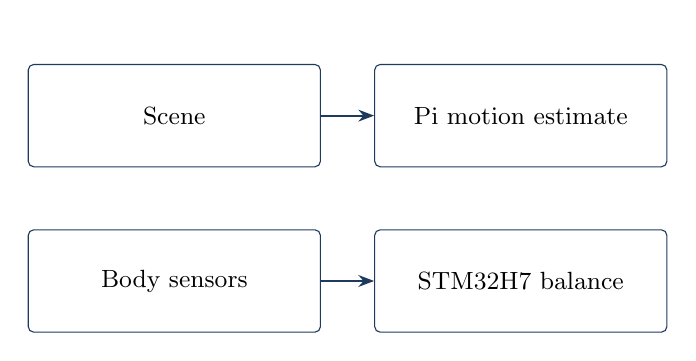
\begin{tikzpicture}[font=\small,box/.append style={font=\small},>=Stealth]\node[box,text width=35mm,minimum height=13mm] (r0n0) at (0.0,0.0) {Scene};\node[box,text width=35mm,minimum height=13mm] (r0n1) at (4.4,0.0) {Pi motion estimate};\draw[flow] (r0n0.east)--(r0n1.west);\node[box,text width=35mm,minimum height=13mm] (r1n0) at (0.0,-2.1) {Body sensors};\node[box,text width=35mm,minimum height=13mm] (r1n1) at (4.4,-2.1) {STM32H7 balance};\draw[flow] (r1n0.east)--(r1n1.west);\node[anchor=west,text=teal!70!black] at (-1.8,1) {};\node[anchor=west,text=muted] at (-1.8,-1.1) {};\end{tikzpicture}}{Navigation and balance use separate sensing paths.}\vfill\takeaway{Loss of perception must leave local balance control running. (Figure~\ref{fig:E3})}\note{Phase 8: docs/ARCHITECTURE.md. experiments/2026-10-14-deck-audit/AUDIT.md. All drawings conceptual unless labeled measured. No gate PASS. }\note{Historical pre-Phase-8 teaching/provenance; latest Phase-8 statements above take precedence. The Pi failure requirement is an ownership invariant, not measured physical stability. Actual geometry, mounting and motion budgets remain unknown. Source register: A. Wheel-biped robot (WBR) perception supports navigation while STM32 retains balance.}\end{frame}
\begin{frame}{2. Controller ownership}\evidence{KNOWN ownership / integration PLANNED}\begin{columns}[T,onlytextwidth]\begin{column}{.43\textwidth}\deckitems{\item Linux runs image processing and mapping.\item STM32H7 owns body estimation, balance and motor safety.\item Navigation references cross only a reviewed boundary.}\end{column}\begin{column}{.53\textwidth}\coursefigure{E13}{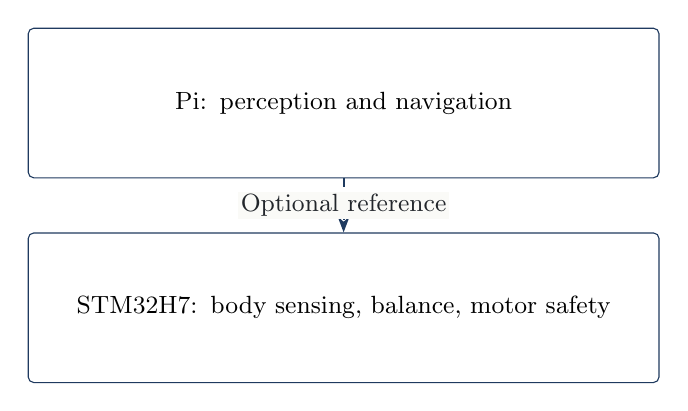
\begin{tikzpicture}[font=\small,box/.append style={font=\small},>=Stealth]\node[box,text width=78mm,minimum height=19mm] (p) at (0,1.2) {Pi: perception and navigation};\node[box,text width=78mm,minimum height=19mm] (s) at (0,-1.4) {STM32H7: body sensing, balance, motor safety};\draw[flow,dashed] (p.south)--node[lbl]{Optional reference}(s.north);\end{tikzpicture}}{The controller retains local authority.}\end{column}\end{columns}\vfill\takeaway{A pose is advice to navigation, never a motor-safety authority. (Figure~\ref{fig:E13})}\note{Phase 8: docs/ARCHITECTURE.md; AGENTS.md. experiments/2026-10-14-deck-audit/AUDIT.md. All drawings conceptual unless labeled measured. No gate PASS. }\note{Historical pre-Phase-8 teaching/provenance; latest Phase-8 statements above take precedence. LQR, VMC and FSM are controller responsibilities, not implemented in this slide task. The actual transport and command envelope remain planned. Physical balance retention still needs approved staged validation. Source register: A,R. Pi owns perception; STM32H7 owns Linear Quadratic Regulator (LQR), Virtual Model Control (VMC), Finite State Machine (FSM), balance and motor safety.}\end{frame}
\begin{frame}{3. Pose usability}\evidence{KNOWN method}\deckitems{\item A pose is an estimated position and orientation.\item Correct-looking numbers may describe old motion or the wrong frame.\item Consumers need age, frame and estimator validity.}\par\vfill\coursefigure{E4}{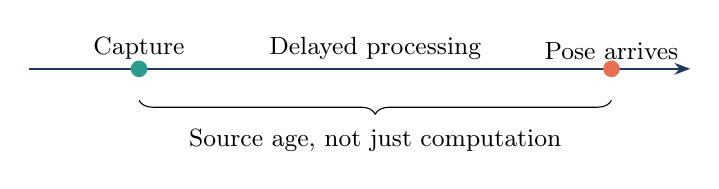
\begin{tikzpicture}[font=\small,box/.append style={font=\small},>=Stealth]\draw[flow] (-.4,0)--(8,0);\node[above] at (1,0){Capture};\node[above] at (4,0){Delayed processing};\node[above] at (7,0){Pose arrives};\fill[teal] (1,0) circle(3pt);\fill[fault] (7,0) circle(3pt);\draw[decorate,decoration={brace,mirror,amplitude=5pt}] (1,-.4)--(7,-.4) node[midway,below=7pt]{Source age, not just computation};\end{tikzpicture}}{Delay can make a plausible pose unusable.}\vfill\takeaway{A recent heartbeat does not establish recent sensor capture. (Figure~\ref{fig:E4})}\note{Phase 8: docs/ARCHITECTURE.md. experiments/2026-10-14-deck-audit/AUDIT.md. All drawings conceptual unless labeled measured. No gate PASS. }\note{Historical pre-Phase-8 teaching/provenance; latest Phase-8 statements above take precedence. Bottom-up qualification separates transport continuity, clock semantics, geometry, algorithm state and receiver policy. No robot safety test has been completed. Source register: A,B. A plausible pose can be stale, misframed or uncalibrated; Linux failure must not remove balance.}\end{frame}
\begin{frame}{4. Session hardware}\evidence{MEASURED boot / final availability UNVERIFIED}\begin{columns}[T,onlytextwidth]\begin{column}{.43\textwidth}\deckitems{\item The 8 GB Pi booted the same 32 GB micro Secure Digital (microSD) card.\item It reported 7.8 GiB memory; under-voltage persisted.\item The 64 GB Universal Serial Bus (USB) stick cannot sustain recording.}\end{column}\begin{column}{.53\textwidth}\coursefigure{E14}{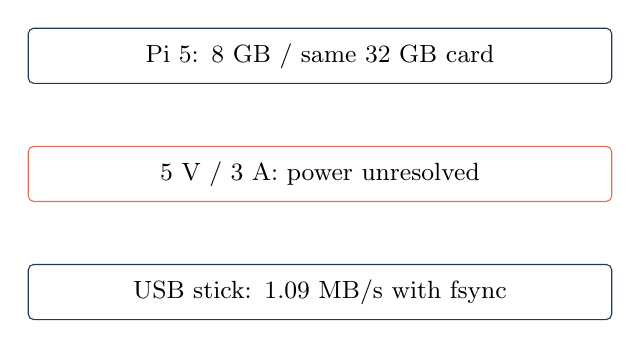
\begin{tikzpicture}[font=\small,box/.append style={font=\small},>=Stealth]\node[box,text width=72mm] (p) at (0,1.2){Pi 5: 8 GB / same 32 GB card};\node[box,text width=72mm,draw=fault] (v) at (0,-.3){5 V / 3 A: power unresolved};\node[box,text width=72mm] (u) at (0,-1.8){USB stick: 1.09 MB/s with fsync};\end{tikzpicture}}{More memory does not repair power or storage.}\end{column}\end{columns}\vfill\takeaway{The ordered 5 A supply and larger card have no qualification evidence. (Figure~\ref{fig:E14})}\note{Phase 8: F14 items 1,6,7; experiments/2026-10-14-SESSION\_FACTS\_ADDENDUM.md; experiments/2026-10-13-SESSION\_FACTS\_FOR\_SLIDES.md. experiments/2026-10-14-deck-audit/AUDIT.md. All drawings conceptual unless labeled measured. No gate PASS. }\note{Historical pre-Phase-8 teaching/provenance; latest Phase-8 statements above take precedence. The active-cooler illustration is conceptual. Historical 13 October: Pi 5 4 GB, 32 GB microSD, 5 V/3 A; source: experiments/2026-10-13-SESSION\_FACTS\_FOR\_SLIDES.md. Historical reports mention different memory inventory and a Raspibase fan. Fresh N0 must record the actual device; do not overwrite history with the target specification. Source register: S,N,PI. Pi 5 8 GB, Ubuntu and Non-Volatile Memory Express (NVMe) storage are the target; actual supply/cooling/storage must be documented anew.}\end{frame}
\begin{frame}{5. D435i sensor inputs}\evidence{MEASURED identity / diagnostic development profile}\begin{columns}[T,onlytextwidth]\begin{column}{.43\textwidth}\deckitems{\item Infrared (IR) left and right images provide stereo views.\item The gyroscope measures angular rate; the accelerometer measures specific force.\item This new camera needs its own calibration and gate evidence.}\end{column}\begin{column}{.53\textwidth}\coursefigure{E9}{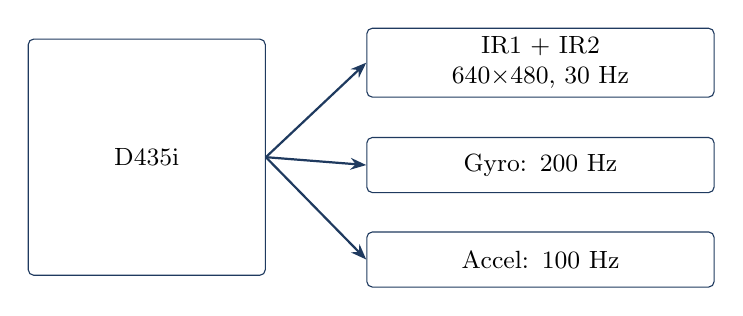
\begin{tikzpicture}[font=\small,box/.append style={font=\small},>=Stealth]\node[box,text width=28mm,minimum height=30mm] (d) at (0,0){D435i};\node[box,text width=42mm] (i) at (5,1.2){IR1 + IR2\\640$\times$480, 30 Hz};\node[box,text width=42mm] (g) at (5,-.1){Gyro: 200 Hz};\node[box,text width=42mm] (a) at (5,-1.3){Accel: 100 Hz};\draw[flow](d.east)--(i.west);\draw[flow](d.east)--(g.west);\draw[flow](d.east)--(a.west);\end{tikzpicture}}{Selected development inputs; the emitter is off.}\end{column}\end{columns}\vfill\takeaway{This paired 30 Hz profile does not replace N2’s IR1/15 profile. (Figure~\ref{fig:E9})}\note{Phase 8: experiments/2026-10-13-SESSION\_FACTS\_FOR\_SLIDES.md section B,E; experiments/2026-10-13-n4b-d435i-prep/n4b\_plan.md. experiments/2026-10-14-deck-audit/AUDIT.md. All drawings conceptual unless labeled measured. No gate PASS. New camera SDK serial 317422076650; ASIC serial 327743061057; USB descriptor serial 327743061057; firmware-update ID is a separate field, not independently established here. Firmware 5.17.3.10; BMI085. Historical SDK 243322073847 and USB descriptor 251843061466 do not transfer N1/N2/calibration receipts.}\note{Historical pre-Phase-8 teaching/provenance; latest Phase-8 statements above take precedence. Active identity: experiments/2026-10-13-SESSION\_FACTS\_FOR\_SLIDES.md, section B. Enumerated 5000 Mbps is not N1 PASS; firmware 5.17.3.10. Historical note follows: Historical 2026-09-13 metadata: firmware 5.17.3.10; SDK serial 243322073847; ASIC serial and firmware-update ID each 251843061466; USB descriptor separately observed. Preserve: IMU Calibration is not available, default intrinsic and extrinsic will be used. These are archived observations, not current enumeration. Source register: RS,C. Two IR views and motion support stereo-inertial inputs; unit historically reports BMI085 despite older BMI055 descriptions.}\end{frame}
\begin{frame}{6. Independent inertial sensors}\evidence{KNOWN method}\deckitems{\item An inertial measurement unit (IMU) combines gyro and acceleration measurements.\item The camera IMU supports visual-inertial estimation.\item The controller body IMU supports local balance.}\par\vfill\coursefigure{E22}{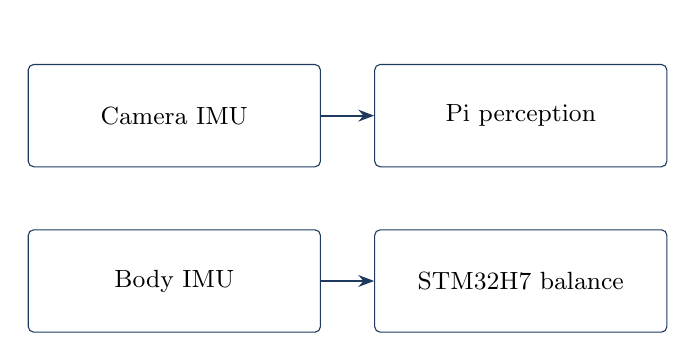
\begin{tikzpicture}[font=\small,box/.append style={font=\small},>=Stealth]\node[box,text width=35mm,minimum height=13mm] (r0n0) at (0.0,0.0) {Camera IMU};\node[box,text width=35mm,minimum height=13mm] (r0n1) at (4.4,0.0) {Pi perception};\draw[flow] (r0n0.east)--(r0n1.west);\node[box,text width=35mm,minimum height=13mm] (r1n0) at (0.0,-2.1) {Body IMU};\node[box,text width=35mm,minimum height=13mm] (r1n1) at (4.4,-2.1) {STM32H7 balance};\draw[flow] (r1n0.east)--(r1n1.west);\node[anchor=west,text=teal!70!black] at (-1.8,1) {};\node[anchor=west,text=muted] at (-1.8,-1.1) {};\end{tikzpicture}}{Different mounts, clocks and calibration; separate jobs.}\vfill\takeaway{Sharing an IMU name does not make the measurements interchangeable. (Figure~\ref{fig:E22})}\note{Phase 8: docs/ARCHITECTURE.md. experiments/2026-10-14-deck-audit/AUDIT.md. All drawings conceptual unless labeled measured. No gate PASS. }\note{Historical pre-Phase-8 teaching/provenance; latest Phase-8 statements above take precedence. Even nominally equal axes and frequencies do not establish synchronization. Do not substitute camera IMU when Pi fails or feed body IMU to ORB without reviewed calibration and clock mapping. Source register: A,C. D435i IMU supplies VIO; STM32 body IMU supplies balance; no naive fusion across independent clocks/mounts.}\end{frame}
\begin{frame}{7. Sensor-to-trajectory paths}\evidence{BUILT direct path / ROS integration PLANNED}\deckitems{\item Programs use the librealsense software development kit (SDK) directly.\item One recording can be replayed repeatedly; live mode bypasses the file.\item Robot Operating System 2 (ROS 2) integration is planned.}\par\vfill\coursefigure{E15}{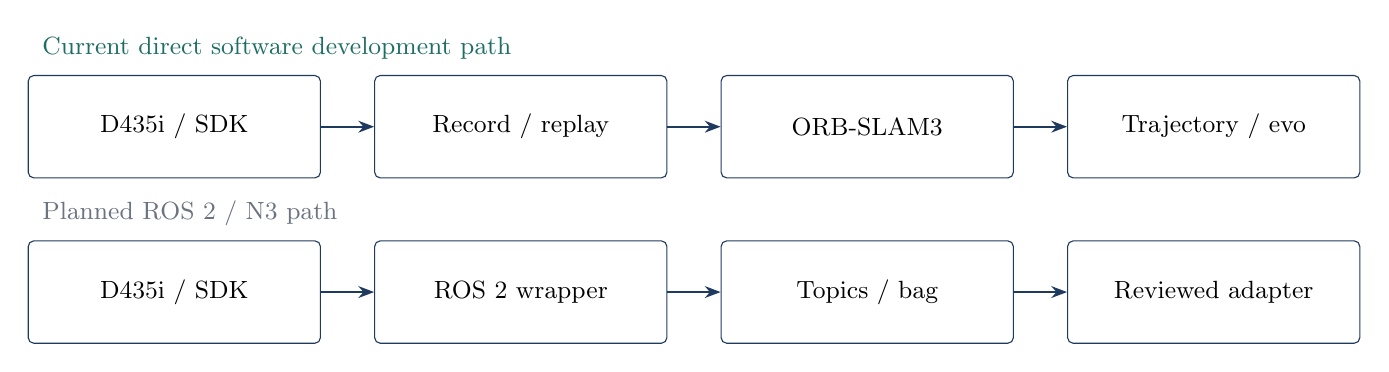
\begin{tikzpicture}[font=\small,box/.append style={font=\small},>=Stealth]\node[box,text width=35mm,minimum height=13mm] (r0n0) at (0.0,0.0) {D435i / SDK};\node[box,text width=35mm,minimum height=13mm] (r0n1) at (4.4,0.0) {Record / replay};\draw[flow] (r0n0.east)--(r0n1.west);\node[box,text width=35mm,minimum height=13mm] (r0n2) at (8.8,0.0) {ORB-SLAM3};\draw[flow] (r0n1.east)--(r0n2.west);\node[box,text width=35mm,minimum height=13mm] (r0n3) at (13.200000000000001,0.0) {Trajectory / evo};\draw[flow] (r0n2.east)--(r0n3.west);\node[box,text width=35mm,minimum height=13mm] (r1n0) at (0.0,-2.1) {D435i / SDK};\node[box,text width=35mm,minimum height=13mm] (r1n1) at (4.4,-2.1) {ROS 2 wrapper};\draw[flow] (r1n0.east)--(r1n1.west);\node[box,text width=35mm,minimum height=13mm] (r1n2) at (8.8,-2.1) {Topics / bag};\draw[flow] (r1n1.east)--(r1n2.west);\node[box,text width=35mm,minimum height=13mm] (r1n3) at (13.200000000000001,-2.1) {Reviewed adapter};\draw[flow] (r1n2.east)--(r1n3.west);\node[anchor=west,text=teal!70!black] at (-1.8,1) {Current direct software development path};\node[anchor=west,text=muted] at (-1.8,-1.1) {Planned ROS 2 / N3 path};\end{tikzpicture}}{Current and planned paths are different implementation stages.}\vfill\takeaway{No successful D435i trajectory is established yet. (Figure~\ref{fig:E15})}\note{Phase 8: experiments/2026-10-13-SESSION\_FACTS\_FOR\_SLIDES.md section E; experiments/2026-10-14-SESSION\_FACTS\_ADDENDUM.md item 5; experiments/2026-10-13-n4b-d435i-prep/n4b\_plan.md. experiments/2026-10-14-deck-audit/AUDIT.md. All drawings conceptual unless labeled measured. No gate PASS. }\note{Historical pre-Phase-8 teaching/provenance; latest Phase-8 statements above take precedence. Source: experiments/2026-09-12-pi5-native-sensor-validation/PHASE\_A\_RUNBOOK.md. Commands are teaching examples only; none executed. UNKNOWN budgets require approval.}\end{frame}
\begin{frame}{8. ROS 2 communication}\evidence{KNOWN ROS concepts / integration PLANNED}\deckitems{\item A publisher sends typed messages on a topic; subscribers receive them.\item Images, IMU samples and poses travel on separate topics.\item Quality of Service (QoS) policies control delivery compatibility.}\par\vfill\coursefigure{E10}{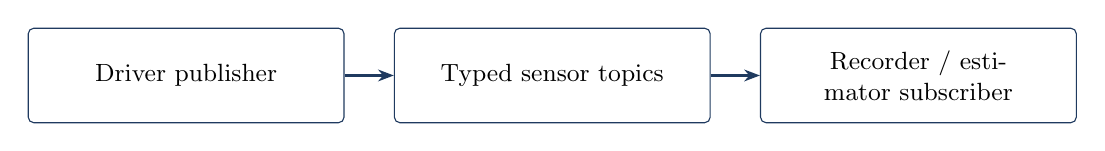
\begin{tikzpicture}[font=\small,box/.append style={font=\small},>=Stealth]\node[box,text width=38mm,minimum height=12mm] (n0) at (0.0,0) {Driver publisher};\node[box,text width=38mm,minimum height=12mm] (n1) at (4.65,0) {Typed sensor topics};\draw[flow] (n0.east)--(n1.west);\node[box,text width=38mm,minimum height=12mm] (n2) at (9.3,0) {Recorder / estimator subscriber};\draw[flow] (n1.east)--(n2.west);\end{tikzpicture}}{ROS 2 connects processes through a message contract.}\vfill\takeaway{Matching topic names alone does not establish compatible delivery. (Figure~\ref{fig:E10})}\note{Phase 8: ROS 2 Jazzy QoS [3]; docs/PERCEPTION\_TOOLING\_ARCHITECTURE.md. experiments/2026-10-14-deck-audit/AUDIT.md. All drawings conceptual unless labeled measured. No gate PASS. }\note{Historical pre-Phase-8 teaching/provenance; latest Phase-8 statements above take precedence. A node is a graph participant; a process can host several nodes and threads. Message header stamps belong to the producer semantics, not automatically to subscription receipt time. Source register: Q,A. Robot Operating System 2 (ROS 2) topics and Data Distribution Service (DDS) transport do not guarantee usable timely data.}\end{frame}
\begin{frame}{9. Pose origin and axes}\evidence{KNOWN method}\deckitems{\item Simultaneous Localization and Mapping (SLAM) estimates pose while building a map.\item The exported trajectory describes camera IMU/body pose in the SLAM world.\item Robot-body pose also needs the mount transform.}\par\vfill\coursefigure{E19}{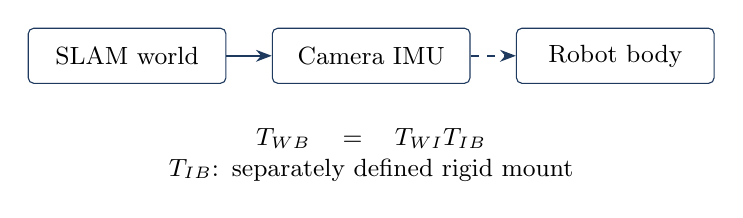
\begin{tikzpicture}[font=\small,box/.append style={font=\small},>=Stealth]\node[box,text width=23mm] (w) at (0,0){SLAM world};\node[box,text width=23mm] (i) at (3.1,0){Camera IMU};\node[box,text width=23mm] (b) at (6.2,0){Robot body};\draw[flow](w.east)--(i.west);\draw[flow,dashed](i.east)--(b.west);\node[below,text width=75mm,align=center] at (3.1,-.8){$T_{WB}=T_{WI}T_{IB}$\\$T_{IB}$: separately defined rigid mount};\end{tikzpicture}}{Compose the estimated sensor pose with a defined mount.}\vfill\takeaway{A camera trajectory is not automatically a robot-body trajectory. (Figure~\ref{fig:E19})}\note{Phase 8: experiments/2026-10-13-n4b-d435i-prep/n4b\_plan.md success observations; docs/ARCHITECTURE.md. experiments/2026-10-14-deck-audit/AUDIT.md. All drawings conceptual unless labeled measured. No gate PASS. }\note{Historical pre-Phase-8 teaching/provenance; latest Phase-8 statements above take precedence. REP-103 conventions are right-handed. REP-105 map can jump; odom is locally continuous but may drift. world is optional and must be explicitly defined. The estimator body means camera IMU coordinates, not the STM32 robot body. Source register: A,TF. The transform (TF) system relates frames; each pose defines parent/child, axes/origin, units and stamp; world/map/odom differ.}\end{frame}
\begin{frame}{10. Stereo geometry}\evidence{KNOWN method}\begin{columns}[T,onlytextwidth]\begin{column}{.43\textwidth}\deckitems{\item Match the same physical point in the two images.\item Horizontal displacement is disparity $d$.\item With focal length $f$ and baseline $b$, depth is $Z=fb/d$.}\end{column}\begin{column}{.53\textwidth}\coursefigure{E6}{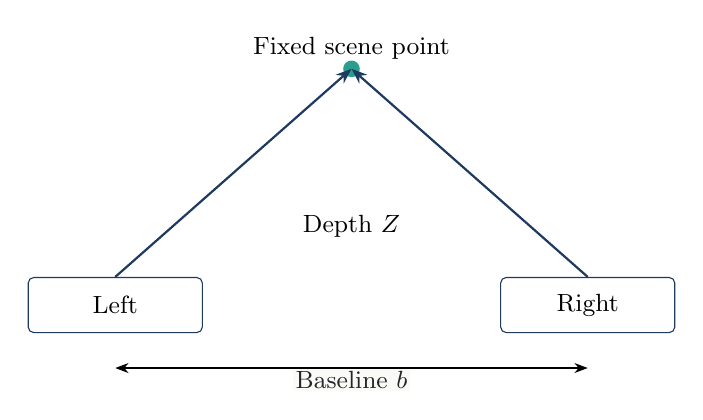
\begin{tikzpicture}[font=\small,box/.append style={font=\small},>=Stealth]\coordinate (p) at (3,3);\node[box,text width=20mm] (l) at (0,0){Left};\node[box,text width=20mm] (r) at (6,0){Right};\fill[teal](p)circle(3pt);\node[above]at(p){Fixed scene point};\draw[flow](l.north)--(p);\draw[flow](r.north)--(p);\draw[<->] (0,-.8)--node[lbl,below]{Baseline $b$}(6,-.8);\node at(3,1){Depth $Z$};\end{tikzpicture}}{Two viewpoints constrain metric depth.}\end{column}\end{columns}\vfill\takeaway{Bad correspondences or calibration yield bad depth. (Figure~\ref{fig:E6})}\note{Phase 8: experiments/2026-10-13-n4b-d435i-prep/n4b\_plan.md; ORB-SLAM3 [1]. experiments/2026-10-14-deck-audit/AUDIT.md. All drawings conceptual unless labeled measured. No gate PASS. }\note{Historical pre-Phase-8 teaching/provenance; latest Phase-8 statements above take precedence. This equation assumes a rectified pinhole pair and nonzero disparity. Here f is focal length in pixels, b is baseline in metres, and Z is metres. No numeric baseline is asserted. See the selected ORB parser and camera profile. Source register: U,RS. Infrared (IR) correspondence and calibrated baseline yield depth; rectification supports reliable pairing.}\end{frame}
\begin{frame}{11. Features constrain motion}\evidence{KNOWN method}\deckitems{\item An image feature is a recognizable corner or local pattern.\item Match fixed scene features across stereo views and later images.\item Many consistent matches constrain camera movement.}\par\vfill\coursefigure{EM1}{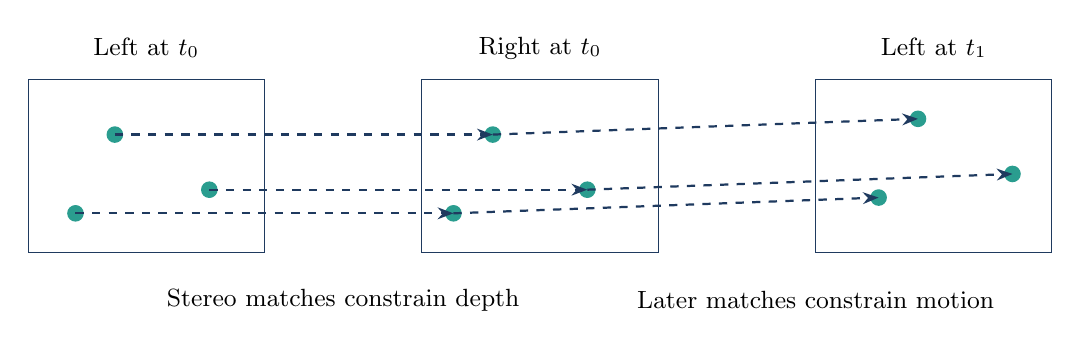
\begin{tikzpicture}[font=\small,box/.append style={font=\small},>=Stealth]\foreach \x/\lab in {0/Left at $t_0$,5/Right at $t_0$,10/Left at $t_1$}{\draw[navy](\x,0)rectangle(\x+3,2.2);\node at(\x+1.5,2.6){\lab};}\foreach \x/\y in {.6/.5,1.1/1.5,2.3/.8}{\fill[teal](\x,\y)circle(3pt);\fill[teal](\x+4.8,\y)circle(3pt);\fill[teal](\x+10.2,\y+.2)circle(3pt);\draw[flow,dashed](\x,\y)--(\x+4.8,\y);\draw[flow,dashed](\x+4.8,\y)--(\x+10.2,\y+.2);}\node at(4,-.6){Stereo matches constrain depth};\node at(10,-.6){Later matches constrain motion};\end{tikzpicture}}{Correspondences link observed pixels to one motion model.}\vfill\takeaway{Track scene features, then test whether their geometry agrees. (Figure~\ref{fig:EM1})}\note{Phase 8: experiments/2026-10-13-n4b-d435i-prep/n4b\_plan.md emitter discussion; retained tracking explanation. experiments/2026-10-14-deck-audit/AUDIT.md. All drawings conceptual unless labeled measured. No gate PASS. }\end{frame}
\begin{frame}{12. Visual and inertial estimation}\evidence{KNOWN method}\begin{columns}[T,onlytextwidth]\begin{column}{.43\textwidth}\deckitems{\item Visual-inertial odometry (VIO) combines both sensor cues.\item IMU prediction bridges image intervals but accumulates drift.\item Image constraints correct that prediction against the scene.}\end{column}\begin{column}{.53\textwidth}\coursefigure{E7}{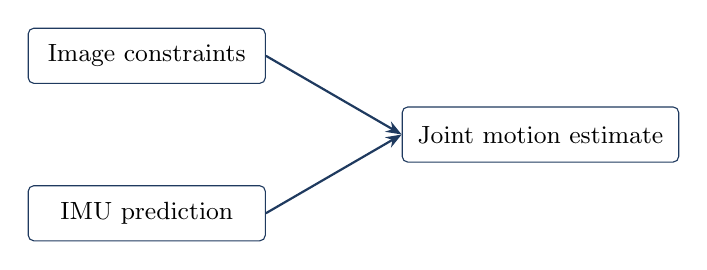
\begin{tikzpicture}[font=\small,box/.append style={font=\small},>=Stealth]\node[box,text width=28mm](v)at(0,1){Image constraints};\node[box,text width=28mm](i)at(0,-1){IMU prediction};\node[box,text width=33mm](p)at(5,0){Joint motion estimate};\draw[flow](v.east)--(p.west);\draw[flow](i.east)--(p.west);\end{tikzpicture}}{Two complementary cues constrain the same motion.}\end{column}\end{columns}\vfill\takeaway{Calibration and timing must connect both measurements correctly. (Figure~\ref{fig:E7})}\note{Phase 8: experiments/2026-10-13-n4b-d435i-prep/n4b\_plan.md; ORB-SLAM3 [1]. experiments/2026-10-14-deck-audit/AUDIT.md. All drawings conceptual unless labeled measured. No gate PASS. }\note{Historical pre-Phase-8 teaching/provenance; latest Phase-8 statements above take precedence. ORB-SLAM3 tightly integrates visual and inertial constraints. The body controller has an independent IMU, mount, clock and calibration. Do not infer integration from shared names. Source register: P,A. Visual-inertial odometry (VIO) combines images with inertial measurement unit (IMU) motion, distinct from body control.}\end{frame}
\begin{frame}{13. Motion between images}\evidence{PREPARED helper / full runtime association UNVERIFIED}\deckitems{\item Gyro and accel samples arrive between successive stereo pairs.\item The helper interpolates accel only within valid gyro-time brackets.\item Preintegration summarizes interval motion before visual correction.}\par\vfill\coursefigure{EM2}{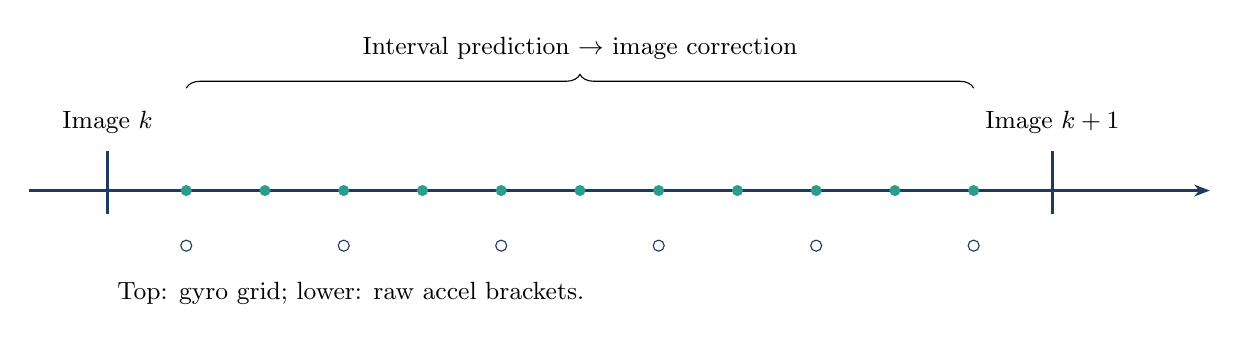
\begin{tikzpicture}[font=\small,box/.append style={font=\small},>=Stealth]\draw[flow](0,0)--(15,0);\foreach \x/\lab in {1/Image $k$,13/Image $k+1$}{\draw[navy,thick](\x,-.3)--(\x,.5);\node[above]at(\x,.6){\lab};}\foreach \x in {2,3,4,5,6,7,8,9,10,11,12}{\fill[teal](\x,0)circle(2pt);}\foreach \x in {2,4,6,8,10,12}{\draw[navy,fill=paper](\x,-.7)circle(2pt);}\node[anchor=west]at(1,-1.3){Top: gyro grid; lower: raw accel brackets.};\draw[decorate,decoration={brace,amplitude=5pt}](2,1.3)--(12,1.3)node[midway,above=7pt]{Interval prediction $\rightarrow$ image correction};\end{tikzpicture}}{Interpolation aligns samples; it creates no new sensor information.}\vfill\takeaway{Reject missing coverage and invalid time steps rather than extrapolating. (Figure~\ref{fig:EM2})}\note{Phase 8: experiments/2026-10-13-SESSION\_FACTS\_FOR\_SLIDES.md section E; experiments/2026-10-13-n4b-d435i-prep/n4b\_plan.md. experiments/2026-10-14-deck-audit/AUDIT.md. All drawings conceptual unless labeled measured. No gate PASS. }\end{frame}
\begin{frame}{14. Tracking}\evidence{KNOWN method}\deckitems{\item Extract and match features from each stereo pair.\item Use the inertial prediction to guide pose estimation.\item Check consistency; update tracking state and select keyframes.}\par\vfill\coursefigure{E33}{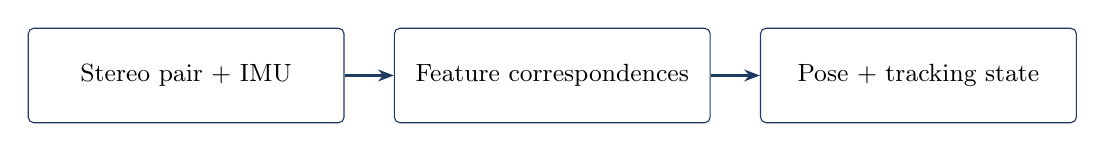
\begin{tikzpicture}[font=\small,box/.append style={font=\small},>=Stealth]\node[box,text width=38mm,minimum height=12mm] (n0) at (0.0,0) {Stereo pair + IMU};\node[box,text width=38mm,minimum height=12mm] (n1) at (4.65,0) {Feature correspondences};\draw[flow] (n0.east)--(n1.west);\node[box,text width=38mm,minimum height=12mm] (n2) at (9.3,0) {Pose + tracking state};\draw[flow] (n1.east)--(n2.west);\end{tikzpicture}}{Tracking estimates the current sensor pose.}\vfill\takeaway{Tracking state is part of the output’s meaning. (Figure~\ref{fig:E33})}\note{Phase 8: ORB-SLAM3 [1]; retained tracking frame. experiments/2026-10-14-deck-audit/AUDIT.md. All drawings conceptual unless labeled measured. No gate PASS. }\note{Historical pre-Phase-8 teaching/provenance; latest Phase-8 statements above take precedence. TrackStereo accepts images, timestamp and vector of IMU measurements. Adapter boundaries need leading and trailing coverage; do not assume example readers guard every boundary. Motion gaps, clock offset, frame error and weak texture require separate diagnosis. Source register: U. Pair stereo images and image-bounded IMU intervals; extract/match features and estimate pose; inspect tracking/reset state before tuning.}\end{frame}
\begin{frame}{15. Keyframes and Atlas}\evidence{KNOWN method}\begin{columns}[T,onlytextwidth]\begin{column}{.43\textwidth}\deckitems{\item A keyframe preserves a useful viewpoint instead of every image.\item Mapping refines keyframe poses and persistent scene points.\item Atlas holds multiple maps; a new map is not seamless tracking.}\end{column}\begin{column}{.53\textwidth}\coursefigure{E34}{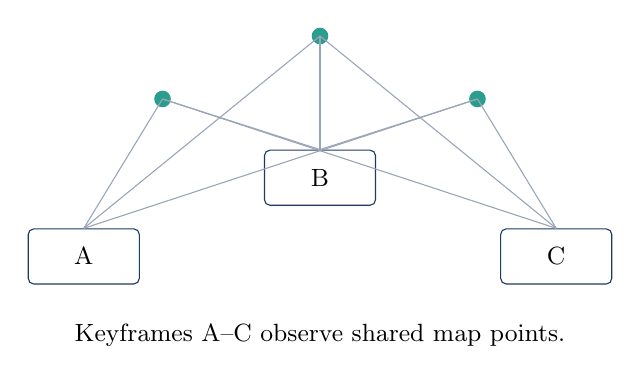
\begin{tikzpicture}[font=\small,box/.append style={font=\small},>=Stealth]\foreach \x/\y/\id in {0/0/A,3/1/B,6/0/C}{\node[box,text width=12mm](\id)at(\x,\y){\id};}\foreach \x/\y in {1/2,3/2.8,5/2}{\fill[teal](\x,\y)circle(3pt);\draw[navy!45](A.north)--(\x,\y);\draw[navy!45](B.north)--(\x,\y);\draw[navy!45](C.north)--(\x,\y);}\node at(3,-1){Keyframes A--C observe shared map points.};\end{tikzpicture}}{Selected views preserve geometric constraints.}\end{column}\end{columns}\vfill\takeaway{Inspect resets and map identity as well as trajectory files. (Figure~\ref{fig:E34})}\note{Phase 8: ORB-SLAM3 [1]. experiments/2026-10-14-deck-audit/AUDIT.md. All drawings conceptual unless labeled measured. No gate PASS. }\note{Historical pre-Phase-8 teaching/provenance; latest Phase-8 statements above take precedence. A keyframe trajectory is not an all-frame trajectory. Compare coverage separately. Mapping load and loop/global optimization can create resource spikes. Preserve map/session/reset identity in the proposed health contract. Source register: P,U. Local optimization estimates map/inertial state; Atlas manages multiple maps/merging; correction can jump the output frame.}\end{frame}
\begin{frame}{16. Algorithm work sharing}\evidence{KNOWN method}\deckitems{\item Tracking handles each incoming image and predicts current pose.\item Local mapping refines nearby keyframes and scene structure.\item Loop closing recognizes revisits and corrects map drift.}\par\vfill\coursefigure{E32}{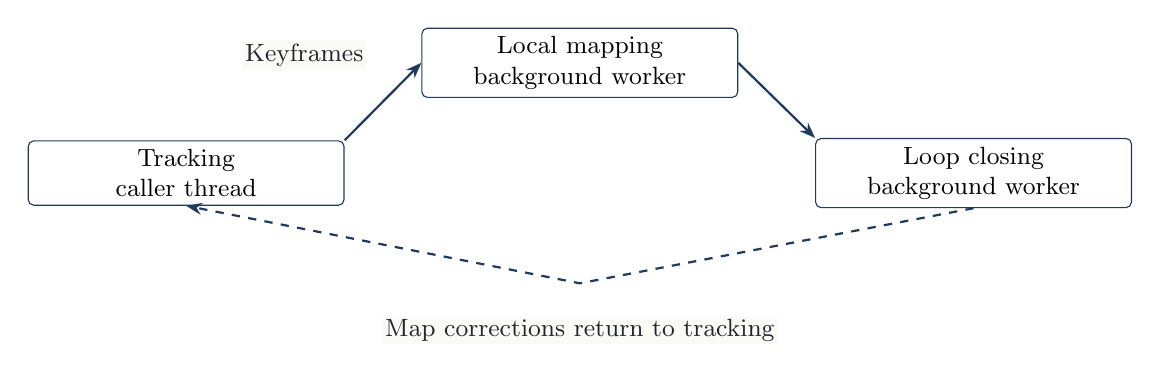
\begin{tikzpicture}[font=\small,box/.append style={font=\small},>=Stealth]\node[box,text width=38mm](t)at(0,0){Tracking\\caller thread};\node[box,text width=38mm](m)at(5,1.4){Local mapping\\background worker};\node[box,text width=38mm](l)at(10,0){Loop closing\\background worker};\draw[flow](t.north east)--(m.west);\node[lbl] at(1.5,1.5){Keyframes};\draw[flow](m.east)--(l.north west);\draw[flow,dashed](l.south)--(5,-1.4)--(t.south);\node[lbl]at(5,-2.0){Map corrections return to tracking};\end{tikzpicture}}{Roles cooperate asynchronously; queueing and scheduling matter.}\vfill\takeaway{Offline playback does not eliminate multithreaded run variation. (Figure~\ref{fig:E32})}\note{Phase 8: ORB-SLAM3 [1]. experiments/2026-10-14-deck-audit/AUDIT.md. All drawings conceptual unless labeled measured. No gate PASS. }\note{Historical pre-Phase-8 teaching/provenance; latest Phase-8 statements above take precedence. FAST means Features from Accelerated Segment Test; BRIEF means Binary Robust Independent Elementary Features. These expansions belong to the feature components. System.cc starts worker threads; tracking and map corrections need explicit event records. The viewer is additional work, not a prerequisite for a scientifically valid display-free output path. Source register: P,U. ORB-SLAM3 uses Oriented FAST and Rotated BRIEF features (expand component names in notes); tracking/mapping/loop closing have distinct roles.}\end{frame}
\begin{frame}{17. Drift and revisits}\evidence{KNOWN method}\begin{columns}[T,onlytextwidth]\begin{column}{.43\textwidth}\deckitems{\item Odometry accumulates local motion errors along a path.\item Loop closure recognizes a previously observed place.\item A map correction can change the global trajectory.}\end{column}\begin{column}{.53\textwidth}\coursefigure{E8}{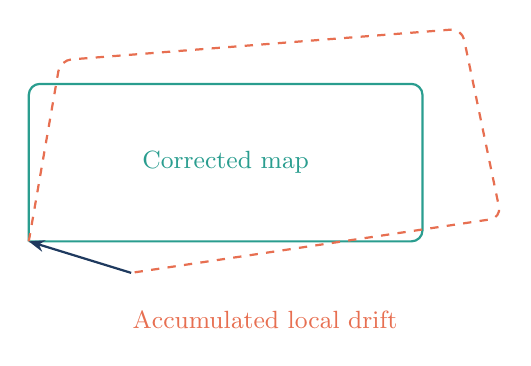
\begin{tikzpicture}[font=\small,box/.append style={font=\small},>=Stealth]\draw[teal,thick,rounded corners] (0,0)--(0,2)--(5,2)--(5,0)--(0,0);\draw[fault,thick,dashed,rounded corners] (0,0)--(.4,2.3)--(5.5,2.7)--(6,.3)--(1.3,-.4);\draw[flow](1.3,-.4)--(0,0);\node[text=teal]at(2.5,1){Corrected map};\node[text=fault]at(3,-1){Accumulated local drift};\end{tikzpicture}}{Conceptual paths, not measured trajectories.}\end{column}\end{columns}\vfill\takeaway{Local continuity and global map correction need different frame semantics. (Figure~\ref{fig:E8})}\note{Phase 8: ROS REP-105 [4]; ORB-SLAM3 [1]. experiments/2026-10-14-deck-audit/AUDIT.md. All drawings conceptual unless labeled measured. No gate PASS. }\note{Historical pre-Phase-8 teaching/provenance; latest Phase-8 statements above take precedence. A planned ROS integration must choose map correction and continuous odometry ownership explicitly. No continuous odometry bridge is implemented or approved. Source register: P,A. Simultaneous localization and mapping (SLAM) adds revisiting and map correction; continuity is a separate requirement.}\end{frame}
\begin{frame}{18. Inertial initialization motion}\evidence{PLANNED diagnostic recipe / not target calibration}\deckitems{\item Initialization estimates gravity, velocity and inertial biases.\item Translate in several directions and rotate the camera.\item Then move through a small loop and finish briefly still.}\par\vfill\coursefigure{E35}{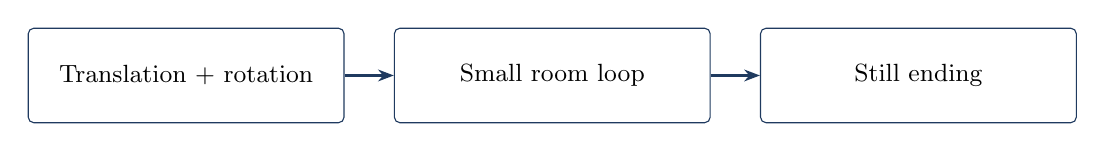
\begin{tikzpicture}[font=\small,box/.append style={font=\small},>=Stealth]\node[box,text width=38mm,minimum height=12mm] (n0) at (0.0,0) {Translation + rotation};\node[box,text width=38mm,minimum height=12mm] (n1) at (4.65,0) {Small room loop};\draw[flow] (n0.east)--(n1.west);\node[box,text width=38mm,minimum height=12mm] (n2) at (9.3,0) {Still ending};\draw[flow] (n1.east)--(n2.west);\end{tikzpicture}}{Diagnostic motion gives the estimator useful excitation.}\vfill\takeaway{Look for IMU initialization; a launch alone is not success. (Figure~\ref{fig:E35})}\note{Phase 8: experiments/2026-10-13-SESSION\_FACTS\_FOR\_SLIDES.md section E; experiments/2026-10-13-n4b-d435i-prep/n4b\_plan.md success observations. experiments/2026-10-14-deck-audit/AUDIT.md. All drawings conceptual unless labeled measured. No gate PASS. }\note{Historical pre-Phase-8 teaching/provenance; latest Phase-8 statements above take precedence. Avoid transferring monocular unknown-scale wording to stereo. Degenerate motion, wrong noise, sign errors and gaps can defeat initialization despite available depth. Initialization criteria and numerical budgets remain planned. Source register: P,U. Estimate gravity, velocity and biases with sufficient excitation; stereo scale does not remove calibration/timing requirements.}\end{frame}
\begin{frame}{19. Infrared projector}\evidence{DEVELOPMENT profile: emitter OFF}\begin{columns}[T,onlytextwidth]\begin{column}{.43\textwidth}\deckitems{\item Tracking needs features belonging to the fixed scene.\item Projected dots depend on the moving camera projector.\item This development path disables the emitter and uses scene texture.}\end{column}\begin{column}{.53\textwidth}\coursefigure{EM3}{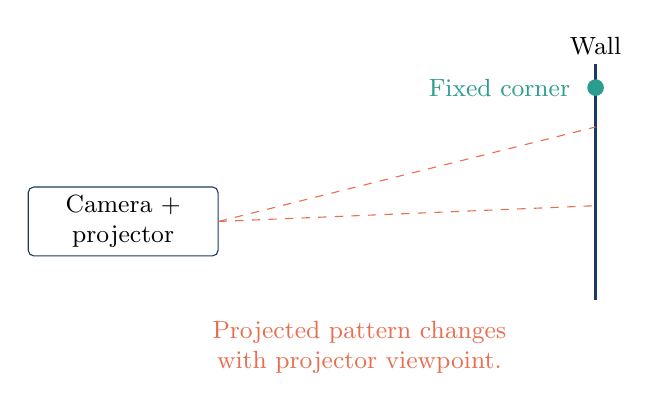
\begin{tikzpicture}[font=\small,box/.append style={font=\small},>=Stealth]\node[box,text width=22mm](c)at(0,0){Camera + projector};\draw[navy,thick](6,-1)--(6,2);\node[above]at(6,2){Wall};\draw[fault,dashed](c.east)--(6,.2);\draw[fault,dashed](c.east)--(6,1.2);\fill[teal](6,1.7)circle(3pt);\node[anchor=east,text=teal]at(5.8,1.7){Fixed corner};\node[text=fault,text width=60mm,align=center]at(3,-1.6){Projected pattern changes with projector viewpoint.};\end{tikzpicture}}{Scene geometry and projected texture are different cues.}\end{column}\end{columns}\vfill\takeaway{Emitter off is a runtime choice; it is not calibration. (Figure~\ref{fig:EM3})}\note{Phase 8: experiments/2026-10-13-SESSION\_FACTS\_FOR\_SLIDES.md section E; experiments/2026-10-13-n4b-d435i-prep/n4b\_plan.md emitter discussion. experiments/2026-10-14-deck-audit/AUDIT.md. All drawings conceptual unless labeled measured. No gate PASS. }\end{frame}
\begin{frame}{20. Calibration questions}\evidence{Calibration unverified}\begin{columns}[T,onlytextwidth]\begin{column}{.43\textwidth}\deckitems{\item Image intrinsics describe projection; stereo extrinsics relate the cameras.\item Camera--IMU geometry is factory nominal; physical alignment is unverified.\item Noise is assumed and time offset remains unknown.}\end{column}\begin{column}{.53\textwidth}\coursefigure{E28}{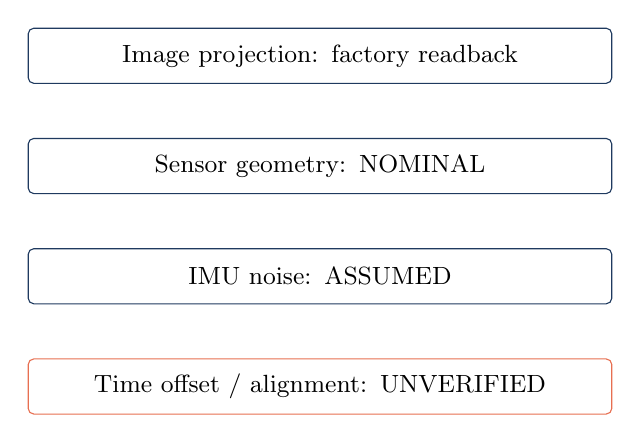
\begin{tikzpicture}[font=\small,box/.append style={font=\small},>=Stealth]\node[box,text width=72mm]at(0,1.8){Image projection: factory readback};\node[box,text width=72mm]at(0,.4){Sensor geometry: NOMINAL};\node[box,text width=72mm]at(0,-1){IMU noise: ASSUMED};\node[box,text width=72mm,draw=fault]at(0,-2.4){Time offset / alignment: UNVERIFIED};\end{tikzpicture}}{Four calibration questions need separate evidence.}\end{column}\end{columns}\vfill\takeaway{A runnable settings file does not establish calibrated VIO. (Figure~\ref{fig:E28})}\note{Phase 8: experiments/2026-10-13-SESSION\_FACTS\_FOR\_SLIDES.md section E; experiments/2026-10-13-n4b-d435i-prep/calibration\_notes.md. experiments/2026-10-14-deck-audit/AUDIT.md. All drawings conceptual unless labeled measured. No gate PASS. Preserve SDK warning: IMU Calibration is not available. Intrinsics and 0.0499 m baseline are factory readback; camera-to-IMU geometry NOMINAL; numeric upstream noise ASSUMED; time offset UNKNOWN.}\note{Historical pre-Phase-8 teaching/provenance; latest Phase-8 statements above take precedence. Current candidate: experiments/2026-10-13-n4b-d435i-prep/D435i\_317422076650\_stereo\_inertial.yaml: nominal factory geometry; noise assumed, not accepted. Preserve verbatim: IMU Calibration is not available, default intrinsic and extrinsic will be used. Historical logs establish CAD fallback, identity sensitivity, zero bias and placeholder zero noise arrays. Do not infer the precise device-side cause from this warning alone. Source register: C. Stereo geometry, camera–IMU extrinsics/time offset and device noise need independent provenance; SDK defaults are not measurements.}\end{frame}
\begin{frame}{21. Stereo rectification}\evidence{KNOWN method}\begin{columns}[T,onlytextwidth]\begin{column}{.43\textwidth}\deckitems{\item Rectification places corresponding points along the same row.\item A wrong image model leaves vertical mismatch or distorted geometry.\item Validate paired pixels before tuning the estimator.}\end{column}\begin{column}{.53\textwidth}\coursefigure{E29}{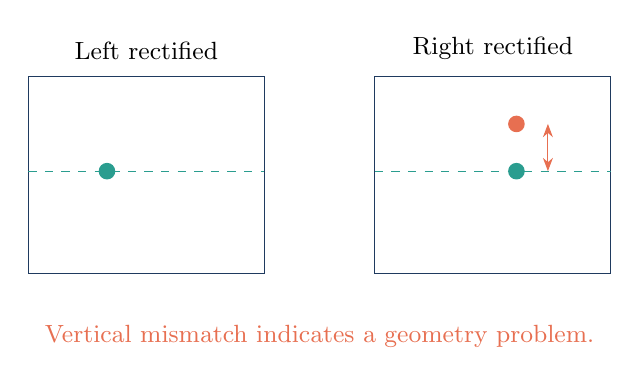
\begin{tikzpicture}[font=\small,box/.append style={font=\small},>=Stealth]\foreach \x/\lab in {0/Left rectified,4.4/Right rectified}{\draw[navy](\x,0)rectangle(\x+3,2.5);\node[above]at(\x+1.5,2.6){\lab};\draw[teal,dashed](\x,1.3)--(\x+3,1.3);}\fill[teal](1,1.3)circle(3pt);\fill[teal](6.2,1.3)circle(3pt);\fill[fault](6.2,1.9)circle(3pt);\draw[fault,<->](6.6,1.3)--(6.6,1.9);\node[text=fault]at(3.7,-.8){Vertical mismatch indicates a geometry problem.};\end{tikzpicture}}{Correct matches share an epipolar row.}\end{column}\end{columns}\vfill\takeaway{Matched rates do not establish matched image geometry. (Figure~\ref{fig:E29})}\note{Phase 8: experiments/2026-10-13-n4b-d435i-prep/calibration\_notes.md; ORB-SLAM3 [1]. experiments/2026-10-14-deck-audit/AUDIT.md. All drawings conceptual unless labeled measured. No gate PASS. }\note{Historical pre-Phase-8 teaching/provenance; latest Phase-8 statements above take precedence. For rectified images corresponding points should lie on the same horizontal epipolar line. Report residual distributions, target coverage, rejected pairs and timestamp differences; budgets require approval. Do not rectify twice or copy EuRoC calibration into D435i settings. Source register: U,K,C. Match chosen profiles/distortion/rectification; inspect epipolar residuals and left/right time pairing before stereo estimation.}\end{frame}
\begin{frame}{22. Three different capture motions}\evidence{PLANNED qualification / diagnostic recipe available}\deckitems{\item Target calibration estimates geometry and camera--IMU timing.\item Room motion tests diagnostic initialization and tracking.\item A stationary noise recording supports Allan analysis.}\par\vfill\coursefigure{E30}{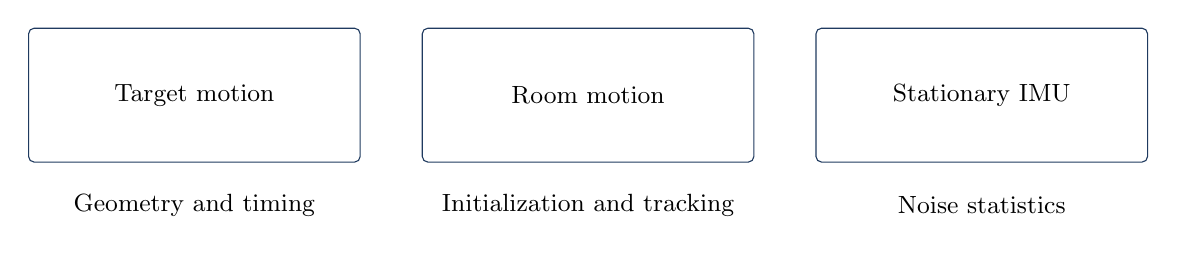
\begin{tikzpicture}[font=\small,box/.append style={font=\small},>=Stealth]\foreach \x/\lab/\purpose in {0/Target motion/Geometry and timing,5/Room motion/Initialization and tracking,10/Stationary IMU/Noise statistics}{\node[box,text width=40mm,minimum height=17mm]at(\x,0){\lab};\node[text width=40mm,align=center]at(\x,-1.4){\purpose};}\end{tikzpicture}}{Different captures answer different engineering questions.}\vfill\takeaway{A successful hand-motion demo does not replace calibration. (Figure~\ref{fig:E30})}\note{Phase 8: experiments/2026-10-13-n4b-d435i-prep/calibration\_notes.md; experiments/2026-10-13-n4b-d435i-prep/n4b\_plan.md. experiments/2026-10-14-deck-audit/AUDIT.md. All drawings conceptual unless labeled measured. No gate PASS. }\note{Historical pre-Phase-8 teaching/provenance; latest Phase-8 statements above take precedence. Kalibr candidate: measured AprilGrid, safe cable slack, varied viewpoints and excitation. Preserve unsuccessful takes. Follow the readiness procedure only after camera authorization and prerequisite gates. No calibration write or guided capture is performed here. Source register: C,K. PLANNED measured AprilGrid and all-axis motion support calibration; textured-room VIO motion has a different purpose.}\end{frame}
\begin{frame}{23. Timestamp clock domains}\evidence{KNOWN method}\begin{columns}[T,onlytextwidth]\begin{column}{.43\textwidth}\deckitems{\item Sensor stamps describe capture in a device clock.\item Host receipt and processing times use a host clock.\item Shared units do not establish shared epochs or drift.}\end{column}\begin{column}{.53\textwidth}\coursefigure{E24}{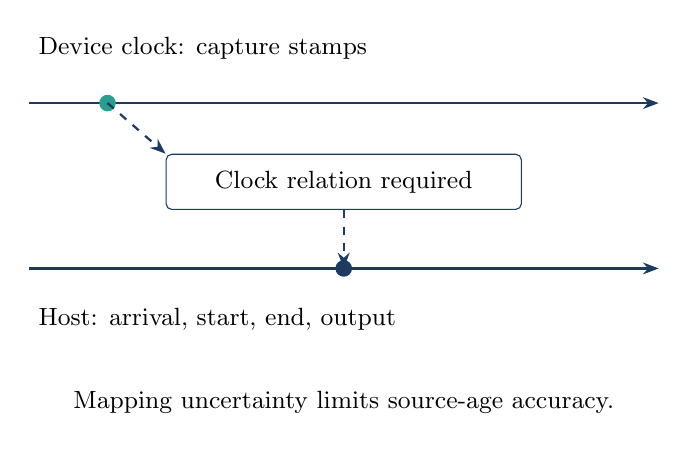
\begin{tikzpicture}[font=\small,box/.append style={font=\small},>=Stealth]\draw[flow](0,1.5)--(8,1.5);\draw[flow](0,-.6)--(8,-.6);\node[anchor=west]at(0,2.2){Device clock: capture stamps};\node[anchor=west]at(0,-1.25){Host: arrival, start, end, output};\fill[teal](1,1.5)circle(3pt);\fill[navy](4,-.6)circle(3pt);\node[box,text width=43mm](m)at(4,.5){Clock relation required};\draw[flow,dashed](1,1.5)--(m.north west);\draw[flow,dashed](m.south)--(4,-.6);\node[text width=77mm,align=center]at(4,-2.3){Mapping uncertainty limits source-age accuracy.};\end{tikzpicture}}{Transport links events, not automatically their clock origins.}\end{column}\end{columns}\vfill\takeaway{Never subtract device capture from host output without a defined relation. (Figure~\ref{fig:E24})}\note{Phase 8: docs/PERCEPTION\_TOOLING\_ARCHITECTURE.md; SDK [5]. experiments/2026-10-14-deck-audit/AUDIT.md. All drawings conceptual unless labeled measured. No gate PASS. }\note{Historical pre-Phase-8 teaching/provenance; latest Phase-8 statements above take precedence. Source: experiments/2026-09-12-pi5-native-sensor-validation/PHASE\_A\_RUNBOOK.md; librealsense v2.58.4 global timestamp reader. Commands are teaching examples only; none executed. UNKNOWN budgets require approval.}\end{frame}
\begin{frame}{24. Queues and backpressure}\evidence{KNOWN method}\deckitems{\item A slow consumer lets old samples accumulate in a queue.\item Blocking may reach acquisition and cause recording gaps.\item Bound queues and make overflow or rejection visible.}\par\vfill\coursefigure{E17}{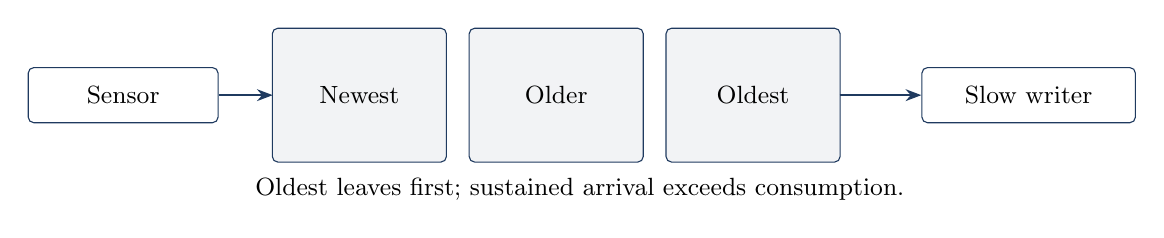
\begin{tikzpicture}[font=\small,box/.append style={font=\small},>=Stealth]\node[box,text width=22mm](s)at(0,0){Sensor};\foreach \x/\lab in {3/Newest,5.5/Older,8/Oldest}{\node[box,fill=navy!6,text width=20mm,minimum height=17mm]at(\x,0){\lab};}\node[box,text width=25mm](c)at(11.5,0){Slow writer};\draw[flow](s.east)--(1.9,0);\draw[flow](9.1,0)--(c.west);\node at(5.8,-1.2){Oldest leaves first; sustained arrival exceeds consumption.};\end{tikzpicture}}{Queue direction follows arrival order and dequeue order.}\vfill\takeaway{Low compute time can coexist with high source age. (Figure~\ref{fig:E17})}\note{Phase 8: experiments/2026-10-13-n4b-d435i-prep/n4b\_plan.md input queues; docs/PERCEPTION\_TOOLING\_ARCHITECTURE.md. experiments/2026-10-14-deck-audit/AUDIT.md. All drawings conceptual unless labeled measured. No gate PASS. }\note{Historical pre-Phase-8 teaching/provenance; latest Phase-8 statements above take precedence. Queue instrumentation is planned. Distinguish producer sequence gaps, observed arrival gaps, recorder count mismatch and measured queue overflow. Latest-only processing may bound age but discards input; inertial coverage must remain consistent. Source register: G,Q,U. Trace SDK/DDS/executor/recorder/estimator queues and policies; unknown drop counters remain UNKNOWN. Merged original page 22: 
\begin{columns}[T,onlytextwidth]\begin{column}{.48\textwidth}\begin{block}{Acquisition / ROS}SDK callbacks deliver sensor frames. Wrapper work and DDS buffering precede the observer and recorder. Each queue can add age or discard input.\end{block}\end{column}\begin{column}{.48\textwidth}\begin{block}{Estimator / Atlas}\texttt{TrackStereo} runs in its caller. Local mapping consumes keyframes; loop closing handles place recognition and map changes. Atlas is shared map state [1].\end{block}\end{column}\end{columns}\medskip Record queue capacity, depth, arrival/dequeue time and discard policy at each owned boundary; unavailable counters stay UNKNOWN.\vfill\takeaway{A recorder count mismatch and a tracking stall can originate in different queues.}Source: experiments/2026-09-12-pi5-native-sensor-validation/PHASE\_A\_RUNBOOK.md; upstream System.cc. Commands are teaching examples only; none executed. UNKNOWN budgets require approval.}\end{frame}
\begin{frame}{25. Recording gaps on the card}\evidence{MEASURED gaps / cause INFERRED}\deckitems{\item The 100 s hand-moved take had 0.3--2.9 s gaps after 22 s.\item Observed file growth was 16.6 MB/s against an 18.4 MB/s input budget.\item Writer stalls blocking acquisition are strongly inferred.}\par\vfill\coursefigure{E18}{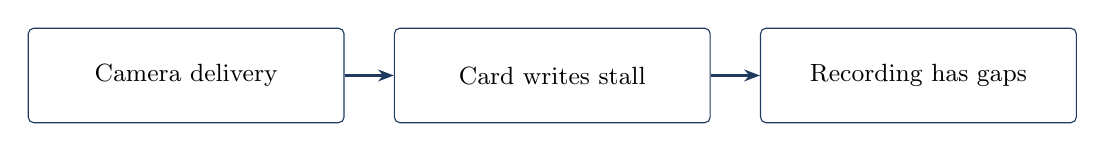
\begin{tikzpicture}[font=\small,box/.append style={font=\small},>=Stealth]\node[box,text width=38mm,minimum height=12mm] (n0) at (0.0,0) {Camera delivery};\node[box,text width=38mm,minimum height=12mm] (n1) at (4.65,0) {Card writes stall};\draw[flow] (n0.east)--(n1.west);\node[box,text width=38mm,minimum height=12mm] (n2) at (9.3,0) {Recording has gaps};\draw[flow] (n1.east)--(n2.west);\end{tikzpicture}}{Observed gaps; storage bottleneck is an inferred cause.}\vfill\takeaway{No USB/power kernel error during this take does not resolve general power. (Figure~\ref{fig:E18})}\note{Phase 8: experiments/2026-10-14-SESSION\_FACTS\_ADDENDUM.md item 3. experiments/2026-10-14-deck-audit/AUDIT.md. All drawings conceptual unless labeled measured. No gate PASS. }\note{Historical pre-Phase-8 teaching/provenance; latest Phase-8 statements above take precedence. Runbook storage proposal: at least 1 GiB and 60 s, overall and worst-batch throughput at least 9.216 decimal MB/s, fsync per 64 MiB batch, SHA-256 readback and finalized cleanup. Default 8 GiB budget may finish too early; a larger write needs review. Retain 10 GiB headroom. No formatting, mounting or storage probe runs here. Source register: G,R. Pin mount source/UUID/device identity and measured throughput/readback; microSD is for operating system and small logs. Merged original page 24: 
\deckitems{\item Y8 stores one eight-bit grayscale byte per pixel; no compression assumed.\item IR1 payload: 640 $\times$ 480 $\times$ 1 $\times$ 15 = 4.608 MB/s.\item Stereo image payload doubles to 9.216 MB/s before overhead.\item Metadata, motion, serialization and filesystem traffic add load.}
\vfill
\begin{block}{Engineering decision}Qualify sustained recording under real load; theoretical USB speed is not available throughput.\end{block}
\vfill\takeaway{Payload arithmetic is a lower bound, not throughput evidence.}
MB uses decimal 1,000,000 bytes. Y8 is eight-bit grayscale. A 300-second IR1 image-payload equivalent is 1.3824 GB; N2 vendor CSV does not actually store those full image pixels. The storage floor 9.216 MB/s is a margin for IR1, not qualification for stereo recording. Source register: G,U. Calculated IR1 payload is 640$\times$480$\times$1$\times$15 = 4.608 decimal MB/s; stereo doubles image payload before overhead.}\end{frame}
\begin{frame}{26. Record in RAM, copy later}\evidence{MEASURED 15 s diagnostic / long take PLANNED}\deckitems{\item Random-access memory (RAM) avoids card writes during capture.\item The 15 s test: IR 29.99 Hz, maximum gap 33 ms, zero observed drops.\item Gyro 200.2 Hz; accel 101 Hz. The later copy passed checksum.}\par\vfill\coursefigure{EM4}{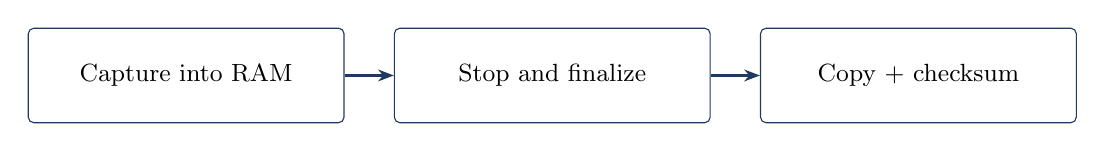
\begin{tikzpicture}[font=\small,box/.append style={font=\small},>=Stealth]\node[box,text width=38mm,minimum height=12mm] (n0) at (0.0,0) {Capture into RAM};\node[box,text width=38mm,minimum height=12mm] (n1) at (4.65,0) {Stop and finalize};\draw[flow] (n0.east)--(n1.west);\node[box,text width=38mm,minimum height=12mm] (n2) at (9.3,0) {Copy + checksum};\draw[flow] (n1.east)--(n2.west);\end{tikzpicture}}{Short RAM test separated capture from slow persistent writes.}\vfill\takeaway{3.9 GB RAM filesystem fits an estimated 1.7 GB take; long reliability is unverified. (Figure~\ref{fig:EM4})}\note{Phase 8: experiments/2026-10-14-SESSION\_FACTS\_ADDENDUM.md item 4. experiments/2026-10-14-deck-audit/AUDIT.md. All drawings conceptual unless labeled measured. No gate PASS. RAM path /dev/shm had 3.9 GB capacity. smoke\_ram.sh is in experiments/2026-10-13-n4b-d435i-prep/. Short test and checksum do not establish 100-second reliability or qualified persistent storage.}\end{frame}
\begin{frame}{27. Camera-independent baseline}\evidence{MEASURED historical 4 GB baseline / N4A OPEN}\deckitems{\item EuRoC MH01 is a public drone dataset with stereo and IMU measurements.\item Ground truth (GT) is independently measured motion used as the reference answer.\item The Pi completed three trials with one map, no resets and IMU initialization.}\par\vfill\coursefigure{E59}{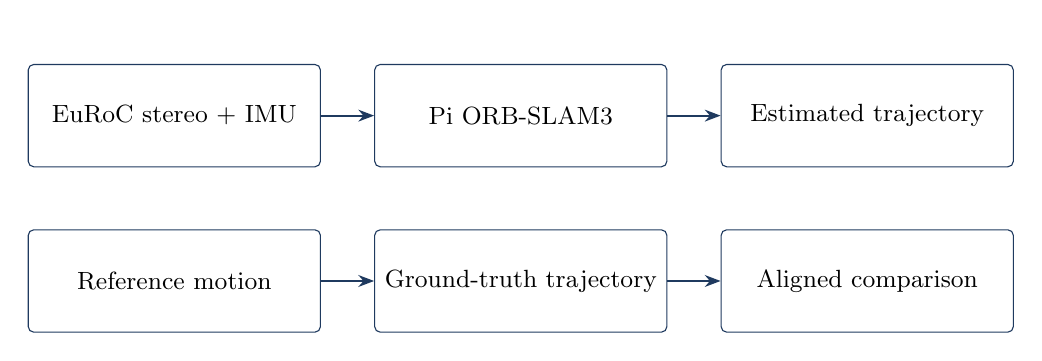
\begin{tikzpicture}[font=\small,box/.append style={font=\small},>=Stealth]\node[box,text width=35mm,minimum height=13mm] (r0n0) at (0.0,0.0) {EuRoC stereo + IMU};\node[box,text width=35mm,minimum height=13mm] (r0n1) at (4.4,0.0) {Pi ORB-SLAM3};\draw[flow] (r0n0.east)--(r0n1.west);\node[box,text width=35mm,minimum height=13mm] (r0n2) at (8.8,0.0) {Estimated trajectory};\draw[flow] (r0n1.east)--(r0n2.west);\node[box,text width=35mm,minimum height=13mm] (r1n0) at (0.0,-2.1) {Reference motion};\node[box,text width=35mm,minimum height=13mm] (r1n1) at (4.4,-2.1) {Ground-truth trajectory};\draw[flow] (r1n0.east)--(r1n1.west);\node[box,text width=35mm,minimum height=13mm] (r1n2) at (8.8,-2.1) {Aligned comparison};\draw[flow] (r1n1.east)--(r1n2.west);\node[anchor=west,text=teal!70!black] at (-1.8,1) {};\node[anchor=west,text=muted] at (-1.8,-1.1) {};\end{tikzpicture}}{Known input separates algorithm/build issues from camera adaptation.}\vfill\takeaway{These completed trials do not establish D435i accuracy or real-time speed. (Figure~\ref{fig:E59})}\note{Phase 8: experiments/2026-10-13-SESSION\_FACTS\_FOR\_SLIDES.md section D; experiments/2026-10-13-n4a-euroc-mh01/REPORT.md; EuRoC [2]. experiments/2026-10-14-deck-audit/AUDIT.md. All drawings conceptual unless labeled measured. No gate PASS. }\note{Historical pre-Phase-8 teaching/provenance; latest Phase-8 statements above take precedence. Source: docs/ORB\_SLAM3\_OFFLINE\_PREPARATION.md; upstream pinned stereo\_inertial\_euroc.cc. Commands are teaching examples only; none executed. UNKNOWN budgets require approval. Merged original page 15: 
\deckitems{\item EuRoC micro aerial vehicle data contain stereo images and IMU. \hyperlink{referencepage}{[2]} \item Published reference trajectories support algorithm evaluation.\item Freeze sequence, calibration and reference association policy.\item A dataset baseline does not qualify Pi camera transport.}
\vfill
\begin{block}{Engineering decision}Compare build/configuration and estimator behavior before involving live capture.\end{block}
\vfill\takeaway{Use known inputs to isolate build and estimator problems.}
Burri et al., 2016. EuRoC references have sequence-dependent motion-capture/laser-tracker limitations. Read known issues and use compatible reference coverage. No dataset download, build or ORB execution is authorized by this deck task. Source register: EU,P. EuRoC micro aerial vehicle data provide stereo, IMU and reference trajectories; these are published dataset properties, not Pi results.}\end{frame}
\begin{frame}{28. Baseline trajectory error}\evidence{MEASURED ATE / N4A qualification OPEN}\deckitems{\item Absolute Trajectory Error (ATE) is position mismatch after aligning the paths.\item Use one rotation and translation, with no scale fitting (SE(3)).\item Root mean square error (RMSE) summarizes the position residuals.}\par\vfill\coursefigure{E80}{\begin{minipage}[c]{.46\linewidth}\centering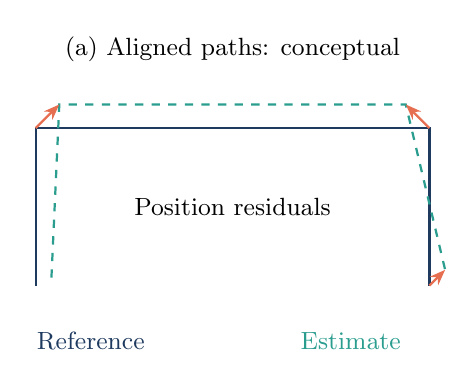
\begin{tikzpicture}[font=\small,box/.append style={font=\small},>=Stealth]\node at(2.5,3){(a) Aligned paths: conceptual};\draw[navy,thick](0,0)--(0,2)--(5,2)--(5,0);\draw[teal,thick,dashed](.2,.1)--(.3,2.3)--(4.7,2.3)--(5.2,.2);\draw[faultflow](0,2)--(.3,2.3);\draw[faultflow](5,2)--(4.7,2.3);\draw[faultflow](5,0)--(5.2,.2);\node at(2.5,1){Position residuals};\node[text=navy]at(.7,-.7){Reference};\node[text=teal]at(4,-.7){Estimate};\end{tikzpicture}\end{minipage}\hfill\begin{minipage}[c]{.48\linewidth}\centering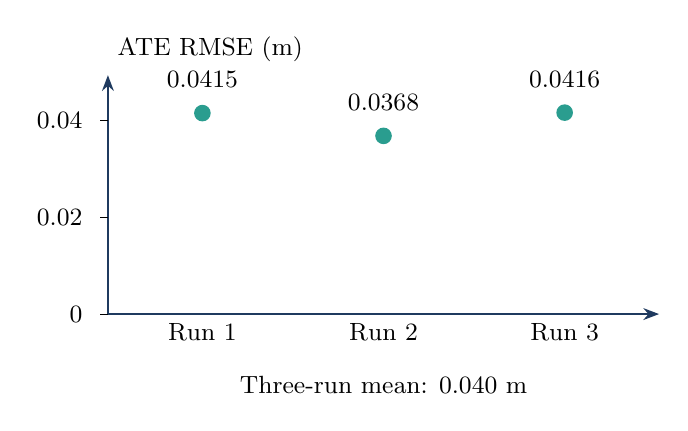
\begin{tikzpicture}[font=\small,box/.append style={font=\small},>=Stealth,y=.82cm]\draw[flow](0,0)--(7,0);\draw[flow](0,0)--(0,3.7);\foreach \y/\lab in {0/0,1.5/0.02,3/0.04}{\draw(0,\y)--(-.1,\y);\node[anchor=east]at(-.2,\y){\lab};}\foreach \x/\y/\v/\r in {1.2/3.1125/0.0415/1,3.5/2.76/0.0368/2,5.8/3.12/0.0416/3}{\fill[teal](\x,\y)circle(3pt);\node[above=2mm]at(\x,\y){\v};\node[below]at(\x,0){Run \r};}\node[anchor=west]at(0,4.1){ATE RMSE (m)};\node at(3.5,-1.1){Three-run mean: 0.040 m};\end{tikzpicture}\end{minipage}}{(a) Residuals after rigid alignment; (b) measured MH01 ATE, no scale fitting.}\vfill\takeaway{About four centimetres on MH01; D435i accuracy remains UNKNOWN. (Figure~\ref{fig:E80})}\note{Phase 8: experiments/2026-10-13-n4a-euroc-mh01/REPORT.md; experiments/2026-10-13-SESSION\_FACTS\_FOR\_SLIDES.md section D; audit: omit unverified paper comparator and RPE. experiments/2026-10-14-deck-audit/AUDIT.md. All drawings conceptual unless labeled measured. No gate PASS. Paper value unverified in the audit source set; comparator omitted. Earlier Phase-7 RPE and extra Sim(3) digits are unverified under this source restriction. Original source/PDF and calculation report remain unchanged; no new evaluation was run.}\note{Historical pre-Phase-8 teaching/provenance; latest Phase-8 statements above take precedence. Evidence: experiments/2026-10-13-n4a-euroc-mh01/REPORT.md; Campos et al., arXiv:2007.11898v2 Table II, prior verification assertion superseded by Phase-8 source restriction. Evidence: slides\_course/qa/n4a-traj-eval-summary.md; tools/trajectory\_eval/README.md. CALCULATED using traj\_eval.py from claude/project-thread-upkfjv, commit d3f9540, PR 2; tool not yet merged. Tool validation passed per its README, not rerun by this deck task. Flags: --t-max-diff 0.02 --t-offset 0 --align-both --rotation-ate --rpe-delta 1 --rpe-unit s. Shared EuRoC clock assumed; offset zero; active body-to-world poses in imu\_body, metres. 3,639 timestamp-associated pose pairs per run. For each eligible start, choose the first later reference timestamp at least 1 s later; no interpolation. SE(3) rigid alignment cancels in RPE. The tool's SE(3) ATE reproduces saved evo scores; its RPE pair policy differs from evo filters. Sim(3) additionally fits scale and is diagnostic, not the stereo-inertial paper comparator. Does not establish frames, extrinsics, synchronization, sensor readiness or gate PASS. No new camera, Pi or ORB execution.}\end{frame}
\begin{frame}{29. Baseline success and camera crash}\evidence{MEASURED crash / rebuild INCOMPLETE}\deckitems{\item Three initial compatibility patches enabled the native build and EuRoC trials.\item Offline D435i replay crashed before the first keyframe.\item Patch 4 initializes the keyframe pointer; rebuilding was interrupted by power loss.}\par\vfill\coursefigure{EM5}{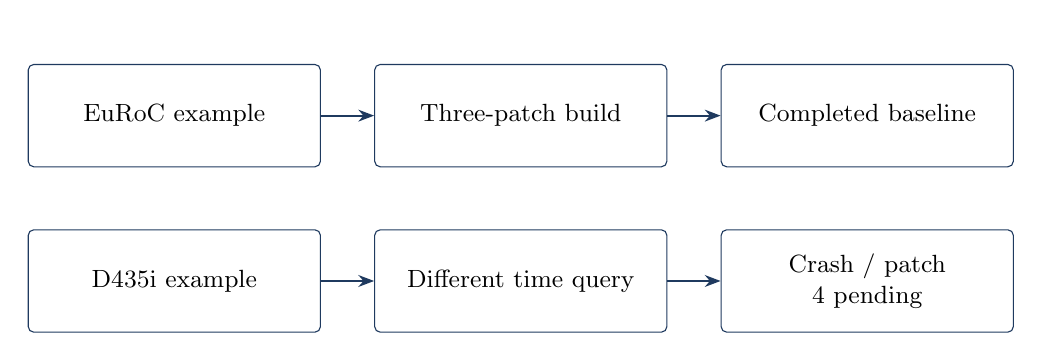
\begin{tikzpicture}[font=\small,box/.append style={font=\small},>=Stealth]\node[box,text width=35mm,minimum height=13mm] (r0n0) at (0.0,0.0) {EuRoC example};\node[box,text width=35mm,minimum height=13mm] (r0n1) at (4.4,0.0) {Three-patch build};\draw[flow] (r0n0.east)--(r0n1.west);\node[box,text width=35mm,minimum height=13mm] (r0n2) at (8.8,0.0) {Completed baseline};\draw[flow] (r0n1.east)--(r0n2.west);\node[box,text width=35mm,minimum height=13mm] (r1n0) at (0.0,-2.1) {D435i example};\node[box,text width=35mm,minimum height=13mm] (r1n1) at (4.4,-2.1) {Different time query};\draw[flow] (r1n0.east)--(r1n1.west);\node[box,text width=35mm,minimum height=13mm] (r1n2) at (8.8,-2.1) {Crash / patch 4 pending};\draw[flow] (r1n1.east)--(r1n2.west);\node[anchor=west,text=teal!70!black] at (-1.8,1) {};\node[anchor=west,text=muted] at (-1.8,-1.1) {};\end{tikzpicture}}{The two examples exercise different code paths.}\vfill\takeaway{A source repair is not a verified executable until rebuilding succeeds. (Figure~\ref{fig:EM5})}\note{Phase 8: experiments/2026-10-13-SESSION\_FACTS\_FOR\_SLIDES.md section C; experiments/2026-10-14-SESSION\_FACTS\_ADDENDUM.md item 5. experiments/2026-10-14-deck-audit/AUDIT.md. All drawings conceptual unless labeled measured. No gate PASS. Initial patches: C++17 and removal of -march=native; Sophus tests disabled after aarch64 array-bounds errors, with headers still used; bool increment replaced by assignment true. D435i gdb stack: main -> System::GetTimeFromIMUInit -> LocalMapping::GetCurrKFTime. Patch 4 initializes KeyFrame* mpCurrentKeyFrame = nullptr in include/LocalMapping.h. EuRoC does not call this query. Power loss interrupted rebuilding after 3 of about 27 objects. Resume command is cmake --build build -j4 in the separate Pi build copy; teaching only, not executed here.}\end{frame}
\begin{frame}{30. Repeatable offline diagnosis}\evidence{MEASURED recording / successful N4B UNVERIFIED}\deckitems{\item The recorder preserves camera samples and timestamps in one file.\item Replay runs the same input without a live acquisition deadline.\item The first offline smoke test crashed; no camera trajectory succeeded.}\par\vfill\coursefigure{E61}{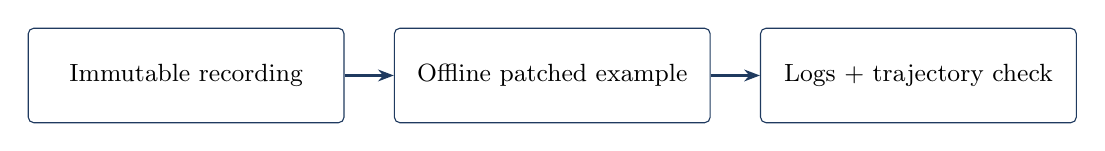
\begin{tikzpicture}[font=\small,box/.append style={font=\small},>=Stealth]\node[box,text width=38mm,minimum height=12mm] (n0) at (0.0,0) {Immutable recording};\node[box,text width=38mm,minimum height=12mm] (n1) at (4.65,0) {Offline patched example};\draw[flow] (n0.east)--(n1.west);\node[box,text width=38mm,minimum height=12mm] (n2) at (9.3,0) {Logs + trajectory check};\draw[flow] (n1.east)--(n2.west);\end{tikzpicture}}{Repeated input isolates estimator changes from acquisition changes.}\vfill\takeaway{Resume and verify patch-4 rebuilding before another diagnostic run. (Figure~\ref{fig:E61})}\note{Phase 8: experiments/2026-10-13-n4b-d435i-prep/n4b\_plan.md; experiments/2026-10-14-SESSION\_FACTS\_ADDENDUM.md items 2--5. experiments/2026-10-14-deck-audit/AUDIT.md. All drawings conceptual unless labeled measured. No gate PASS. }\note{Historical pre-Phase-8 teaching/provenance; latest Phase-8 statements above take precedence. Evidence: experiments/2026-10-13-SESSION\_FACTS\_FOR\_SLIDES.md; experiments/2026-10-13-n4b-d435i-prep/n4b\_plan.md. Deck authoring only; no camera, Pi or ORB program was executed in Phase 6.}\end{frame}
\begin{frame}{31. Live freshness}\evidence{PLANNED live diagnostic / N4C OPEN}\begin{columns}[T,onlytextwidth]\begin{column}{.43\textwidth}\deckitems{\item Live estimation must consume new data as it arrives.\item Queue growth can make an otherwise accurate pose stale.\item No successful live estimator run is documented; rebuild is incomplete.}\end{column}\begin{column}{.53\textwidth}\coursefigure{E64}{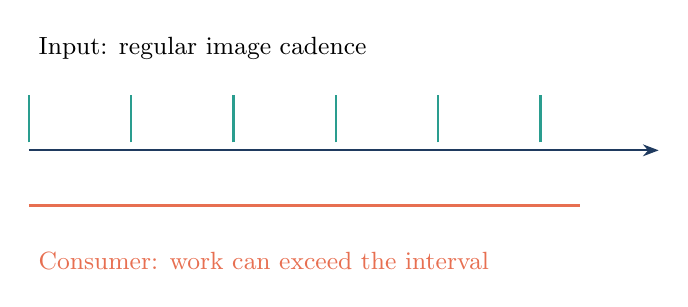
\begin{tikzpicture}[font=\small,box/.append style={font=\small},>=Stealth]\draw[flow](0,0)--(8,0);\foreach \x in {0,1.3,2.6,3.9,5.2,6.5}{\draw[teal,thick](\x,.1)--(\x,.7);}\draw[fault,thick](0,-.7)--(7,-.7);\node[anchor=west]at(0,1.3){Input: regular image cadence};\node[anchor=west,text=fault]at(0,-1.4){Consumer: work can exceed the interval};\end{tikzpicture}}{A conceptual overload timeline; no latency measurement.}\end{column}\end{columns}\vfill\takeaway{Measure age, queueing and drops after offline diagnosis succeeds. (Figure~\ref{fig:E64})}\note{Phase 8: experiments/2026-10-14-SESSION\_FACTS\_ADDENDUM.md item 5; experiments/2026-10-13-n4b-d435i-prep/n4b\_plan.md. experiments/2026-10-14-deck-audit/AUDIT.md. All drawings conceptual unless labeled measured. No gate PASS. }\note{Historical pre-Phase-8 teaching/provenance; latest Phase-8 statements above take precedence. Evidence: experiments/2026-10-13-SESSION\_FACTS\_FOR\_SLIDES.md; experiments/2026-10-13-n4b-d435i-prep/n4b\_plan.md. Deck authoring only; no camera, Pi or ORB program was executed in Phase 6.}\end{frame}
\begin{frame}{32. Bottom-up diagnosis}\evidence{KNOWN method}\deckitems{\item Identify the earliest failed layer before tuning later layers.\item A recording gap starts with delivery/storage checks.\item A first-frame crash starts with its stack trace and build identity.}\par\vfill\coursefigure{E73}{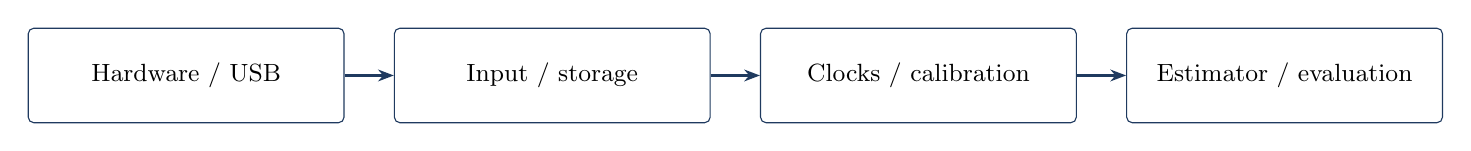
\begin{tikzpicture}[font=\small,box/.append style={font=\small},>=Stealth]\node[box,text width=38mm,minimum height=12mm] (n0) at (0.0,0) {Hardware / USB};\node[box,text width=38mm,minimum height=12mm] (n1) at (4.65,0) {Input / storage};\draw[flow] (n0.east)--(n1.west);\node[box,text width=38mm,minimum height=12mm] (n2) at (9.3,0) {Clocks / calibration};\draw[flow] (n1.east)--(n2.west);\node[box,text width=38mm,minimum height=12mm] (n3) at (13.950000000000001,0) {Estimator / evaluation};\draw[flow] (n2.east)--(n3.west);\end{tikzpicture}}{Earlier failures invalidate conclusions from later layers.}\vfill\takeaway{Preserve raw warnings and failed runs while isolating the cause. (Figure~\ref{fig:E73})}\note{Phase 8: experiments/2026-10-14-SESSION\_FACTS\_ADDENDUM.md items 3--5; docs/PERCEPTION\_TOOLING\_ARCHITECTURE.md. experiments/2026-10-14-deck-audit/AUDIT.md. All drawings conceptual unless labeled measured. No gate PASS. }\note{Historical pre-Phase-8 teaching/provenance; latest Phase-8 statements above take precedence. Bottom-up order reduces ambiguity. Save complete logs before changing one variable. Use recorded inputs to separate acquisition from estimator behavior; add only instrumentation needed to answer the bounded question. Source register: A,H,G. Hardware$\rightarrow$USB$\rightarrow$raw$\rightarrow$clocks$\rightarrow$driver$\rightarrow$ROS$\rightarrow$QoS$\rightarrow$calibration$\rightarrow$ORB-SLAM3$\rightarrow$trajectory$\rightarrow$evaluation; fix first failed layer. Merged original page 85: 
\deckitems{\item 480M: inspect cable, direct branch and power before software.\item Silent topic: inspect publisher, parameter readback and QoS.\item Initialization failure: inspect coverage, frames, offset and noise.\item Calibration fallback: preserve warning; do not copy constants.}
\vfill
\begin{tabular}{L{87.0mm}L{87.0mm}}\toprule
\textbf{Symptom} & \textbf{First discriminating evidence}\\\midrule
480M / disconnect & Own branch + power/kernel logs\\[5pt]
Topic silence & Graph + readback + QoS\\[5pt]
Loss / failed initialization & Pairing + motion coverage + calibration\\[5pt]
\bottomrule\end{tabular}
\vfill\takeaway{Similar symptoms can require different evidence.}
Permissions need exact device-ancestor inspection, not broad access. If trajectory looks smooth, still inspect stale epochs, reset state and reference coverage. A storage bottleneck can manifest as delayed recording without raw sensor failure. Diagnose one layer at a time. Source register: H,E,C. USB2/power/permissions/topic silence/bad association/calibration fallback need different evidence and remedies.}\end{frame}
\begin{frame}{33. Health supervision}\evidence{Integration PLANNED / no physical safety verdict}\begin{columns}[T,onlytextwidth]\begin{column}{.43\textwidth}\deckitems{\item A heartbeat says a process is alive, not that its pose is fresh.\item A planned receiver checks source age, validity and session identity.\item Stale or invalid perception withdraws optional navigation input.}\end{column}\begin{column}{.53\textwidth}\coursefigure{E40}{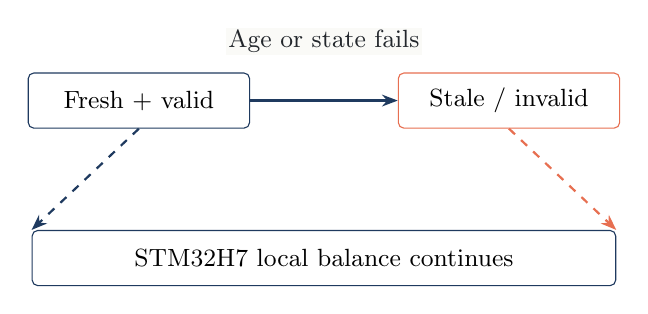
\begin{tikzpicture}[font=\small,box/.append style={font=\small},>=Stealth]\node[box,text width=26mm](f)at(0,0){Fresh + valid};\node[box,text width=26mm,draw=fault](h)at(4.7,0){Stale / invalid};\draw[flow](f.east)--(h.west);\node[lbl]at(2.35,.75){Age or state fails};\node[box,text width=72mm](s)at(2.35,-2){STM32H7 local balance continues};\draw[flow,dashed](f.south)--(s.north west);\draw[faultflow,dashed](h.south)--(s.north east);\end{tikzpicture}}{Navigation validity is supervised separately from balance.}\end{column}\end{columns}\vfill\takeaway{Rates, age budgets and message design still require review. (Figure~\ref{fig:E40})}\note{Phase 8: docs/ARCHITECTURE.md. experiments/2026-10-14-deck-audit/AUDIT.md. All drawings conceptual unless labeled measured. No gate PASS. }\note{Historical pre-Phase-8 teaching/provenance; latest Phase-8 statements above take precedence. This is a planned semantic state model, not firmware. Wrong frame, nonfinite fields, duplicate sequence, old session and unannounced map jump must reject. Receiver clock wrap, mapping uncertainty and restart behavior need reviewed fixtures. Source register: A,B. PLANNED absent/initializing/fresh/stale/invalid transitions require receiver checks; heartbeat does not prove source freshness.}\end{frame}
\begin{frame}{34. Different evidence branches}\evidence{MEASURED diagnostics / all gates OPEN}N4A tests known data; camera qualification follows N0 $\rightarrow$ N1 $\rightarrow$ N2 $\rightarrow$ N3. No gate has PASSED.\par\medskip Exact N2 raw profile: IR1 Y8 640$\times$480/15, gyro/200, accel/100.\par\vfill\coursefigure{E42}{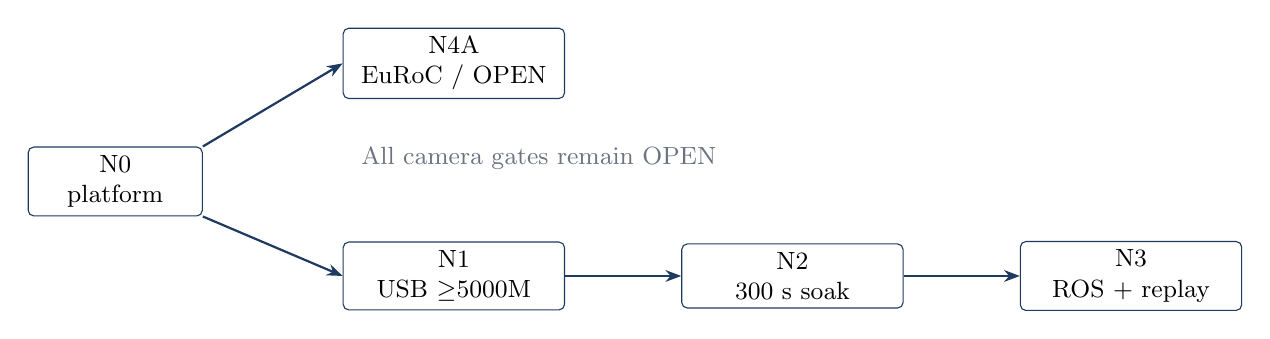
\begin{tikzpicture}[font=\small,box/.append style={font=\small},>=Stealth]\node[box,text width=20mm](n0)at(0,0){N0\\platform};\node[box,text width=26mm](a)at(4.3,1.5){N4A\\EuRoC / OPEN};\node[box,text width=26mm](n1)at(4.3,-1.2){N1\\USB $\geq$5000M};\node[box,text width=26mm](n2)at(8.6,-1.2){N2\\300 s soak};\node[box,text width=26mm](n3)at(12.9,-1.2){N3\\ROS + replay};\draw[flow](n0.north east)--(a.west);\draw[flow](n0.south east)--(n1.west);\draw[flow](n1.east)--(n2.west);\draw[flow](n2.east)--(n3.west);\node[anchor=west,text=muted]at(3,.3){All camera gates remain OPEN};\end{tikzpicture}}{Dataset results do not qualify new-camera transport or timing.}\vfill\takeaway{The 15 s RAM test cannot replace the mandatory 300-second N2 soak. (Figure~\ref{fig:E42})}\note{Phase 8: experiments/2026-10-14-SESSION\_FACTS\_ADDENDUM.md; experiments/2026-10-13-n4b-d435i-prep/n4b\_plan.md exact N2 requirements. experiments/2026-10-14-deck-audit/AUDIT.md. All drawings conceptual unless labeled measured. No gate PASS. }\note{Historical pre-Phase-8 teaching/provenance; latest Phase-8 statements above take precedence. Source: BRIEF.md; Phase A runbook; offline preparation. Commands are teaching examples only; none executed. UNKNOWN budgets require approval.}\end{frame}
\begin{frame}{35. Established work and open gaps}\evidence{MEASURED progress / power UNRESOLVED}\deckitems{\item Established: 8 GB boot, EuRoC trials and short RAM recording.\item Open: power, long capture, patch-4 rebuild and calibrated camera tracking.\item Later Wi-Fi reachability failed; final operating state is unverified.}\par\vfill\coursefigure{E87}{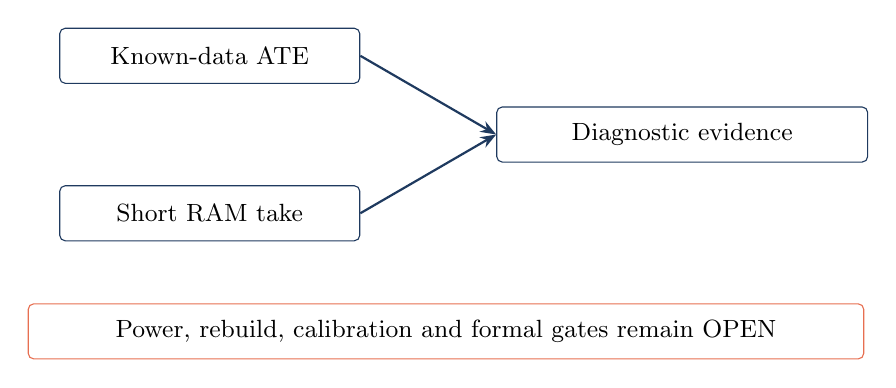
\begin{tikzpicture}[font=\small,box/.append style={font=\small},>=Stealth]\node[box,text width=36mm](a)at(0,1){Known-data ATE};\node[box,text width=36mm](r)at(0,-1){Short RAM take};\node[box,text width=45mm](e)at(6,0){Diagnostic evidence};\draw[flow](a.east)--(e.west);\draw[flow](r.east)--(e.west);\node[box,draw=fault,text width=104mm]at(3,-2.5){Power, rebuild, calibration and formal gates remain OPEN};\end{tikzpicture}}{Useful observations coexist with unresolved qualification.}\vfill\takeaway{Neither larger RAM nor a clean short take establishes robot readiness. (Figure~\ref{fig:E87})}\note{Phase 8: experiments/2026-10-14-SESSION\_FACTS\_ADDENDUM.md items 1--7; experiments/2026-10-13-n4a-euroc-mh01/REPORT.md. experiments/2026-10-14-deck-audit/AUDIT.md. All drawings conceptual unless labeled measured. No gate PASS. }\note{Historical pre-Phase-8 teaching/provenance; latest Phase-8 statements above take precedence. Evidence: experiments/2026-10-13-SESSION\_FACTS\_FOR\_SLIDES.md; experiments/2026-10-13-n4a-euroc-mh01/REPORT.md. Deck authoring only; no camera, Pi or ORB program was executed in Phase 6.}\end{frame}
\begin{frame}{36. Next diagnostic sequence}\evidence{PLANNED / diagnostic only}After explicit CAMERA AVAILABLE authorization, the addendum proposes this diagnostic sequence. It does not bypass formal N1 $\rightarrow$ N2 $\rightarrow$ N3 qualification.\par\vfill\coursefigure{E89}{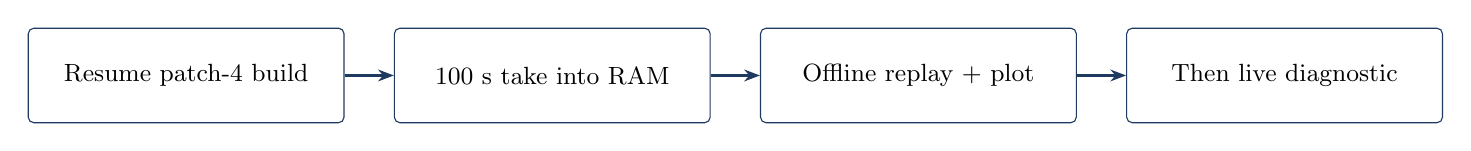
\begin{tikzpicture}[font=\small,box/.append style={font=\small},>=Stealth]\node[box,text width=38mm,minimum height=12mm] (n0) at (0.0,0) {Resume patch-4 build};\node[box,text width=38mm,minimum height=12mm] (n1) at (4.65,0) {100 s take into RAM};\draw[flow] (n0.east)--(n1.west);\node[box,text width=38mm,minimum height=12mm] (n2) at (9.3,0) {Offline replay + plot};\draw[flow] (n1.east)--(n2.west);\node[box,text width=38mm,minimum height=12mm] (n3) at (13.950000000000001,0) {Then live diagnostic};\draw[flow] (n2.east)--(n3.west);\end{tikzpicture}}{Proposed sequence, not executed in deck authoring.}\vfill\takeaway{Stable power and calibration remain prerequisites to qualification. (Figure~\ref{fig:E89})}\note{Phase 8: experiments/2026-10-14-SESSION\_FACTS\_ADDENDUM.md tomorrow plan; experiments/2026-10-13-n4b-d435i-prep/n4b\_plan.md. experiments/2026-10-14-deck-audit/AUDIT.md. All drawings conceptual unless labeled measured. No gate PASS. }\note{Historical pre-Phase-8 teaching/provenance; latest Phase-8 statements above take precedence. The roadmap is conditional. Earlier transport gates block physical acquisition; independent algorithm planning remains useful but no ORB execution is authorized now. Preserve every failure and ask for the missing decision only when concrete evidence is ready. Source register: B,O,G. Fresh N0$\rightarrow$N1$\rightarrow$N2$\rightarrow$N3, reviewed stereo/calibration extension, N4A/B/C$\rightarrow$N5$\rightarrow$N6$\rightarrow$N7; blockers yield records, not deadline promises.}\end{frame}
\begin{frame}{37. Current system claim}\evidence{MEASURED baseline / integration PLANNED}\deckitems{\item The Pi build estimated motion on known EuRoC input with about 4 cm ATE.\item Camera recording improved in a short RAM test; camera estimation remains unverified.\item STM32H7 retains local balance and motor-safety ownership.}\par\vfill\coursefigure{E90}{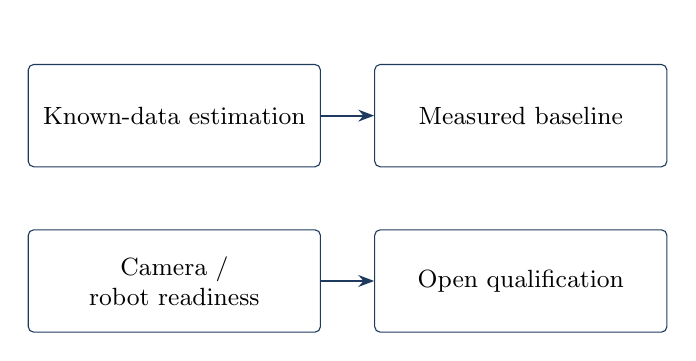
\begin{tikzpicture}[font=\small,box/.append style={font=\small},>=Stealth]\node[box,text width=35mm,minimum height=13mm] (r0n0) at (0.0,0.0) {Known-data estimation};\node[box,text width=35mm,minimum height=13mm] (r0n1) at (4.4,0.0) {Measured baseline};\draw[flow] (r0n0.east)--(r0n1.west);\node[box,text width=35mm,minimum height=13mm] (r1n0) at (0.0,-2.1) {Camera / robot readiness};\node[box,text width=35mm,minimum height=13mm] (r1n1) at (4.4,-2.1) {Open qualification};\draw[flow] (r1n0.east)--(r1n1.west);\node[anchor=west,text=teal!70!black] at (-1.8,1) {};\node[anchor=west,text=muted] at (-1.8,-1.1) {};\end{tikzpicture}}{Progress and readiness answer different questions.}\vfill\takeaway{Resume the repair and diagnostic sequence while keeping every gate OPEN. (Figure~\ref{fig:E90})}\note{Phase 8: experiments/2026-10-14-SESSION\_FACTS\_ADDENDUM.md; experiments/2026-10-13-n4a-euroc-mh01/REPORT.md; docs/ARCHITECTURE.md. experiments/2026-10-14-deck-audit/AUDIT.md. All drawings conceptual unless labeled measured. No gate PASS. }\note{Historical pre-Phase-8 teaching/provenance; latest Phase-8 statements above take precedence. Contribution: one source-grounded gate ladder, ownership boundary, implementation/data/clock model, evaluation contract and bounded AI tickets. The owner can direct agents without conflating tooling tests and hardware evidence. Physical balance and performance remain unverified. Source register: A,B,G. Trust needs qualified acquisition/timing/calibration/repeated estimation; controller independence protects balance; next step is N0 evidence.}\end{frame}
\begin{frame}{References}\hypertarget{referencepage}{}\footnotesize\begin{columns}[T,onlytextwidth]
\begin{column}{.48\textwidth}
\par\medskip\textbf{[1]} Campos, Elvira, Gómez Rodríguez, Montiel, Tardós. ORB-SLAM3. arXiv:2007.11898v2, 2021. \href{https://arxiv.org/abs/2007.11898}{Primary source}.
\par\medskip\textbf{[2]} Burri et al. The EuRoC micro aerial vehicle datasets. International Journal of Robotics Research, 2016. \href{https://projects.asl.ethz.ch/datasets/euroc-mav/}{Primary source}.
\par\medskip\textbf{[3]} ROS 2 Jazzy: Quality of Service documentation. \href{https://docs.ros.org/en/jazzy/Concepts/Intermediate/About-Quality-of-Service-Settings.html}{Primary source}.
\par\medskip\textbf{[4]} ROS REP-103 / REP-105: units, coordinates and frames. \href{https://www.ros.org/reps/rep-0105.html}{Primary source}.
\par\medskip\textbf{[5]} RealSense librealsense v2.58.4: timestamp reader and calibration parser. \href{https://github.com/realsenseai/librealsense/tree/v2.58.4}{Primary source}.
\end{column}
\begin{column}{.48\textwidth}
\par\medskip\textbf{[6]} ETH Zürich ASL: Kalibr camera–IMU calibration. \href{https://github.com/ethz-asl/kalibr/wiki/camera-imu-calibration}{Primary source}.
\par\medskip\textbf{[7]} gaowenliang: imu\_utils maintainer documentation. \href{https://github.com/gaowenliang/imu_utils}{Primary source}.
\par\medskip\textbf{[8]} Michael Grupp: evo trajectory metrics. \href{https://github.com/MichaelGrupp/evo/wiki/Metrics}{Primary source}.
\par\medskip\textbf{[9]} Raspberry Pi 5 / Active Cooler and RealSense D435i vendor records. \href{https://www.raspberrypi.com/products/raspberry-pi-5/}{Primary source}. \href{https://www.intel.com/content/www/us/en/products/sku/190004/intel-realsense-depth-camera-d435i/specifications.html}{D435i record}.
\end{column}
\end{columns}\vfill\normalsize N4A accuracy is measured; D435i and robot qualification remain OPEN.\end{frame}
\appendix
% BACKUP GROUP: Gate acceptance and diagnosis
\begin{frame}{Backup: 4.2 N0: acceptance and diagnosis}\evidence{PLANNED / no gate PASS}
ARM64: 64-bit Arm; OS: operating system; UTC: Coordinated Universal Time.\par\medskip\begin{tabular}{@{}L{80mm}L{104mm}@{}}\toprule
\textbf{PASS requirement} & \textbf{Measurement / clock}\\\midrule
ARM64; Ubuntu 24.04; Jazzy & OS/package inventory; observation UTC\\[6pt]
UTC synchronized; flags 0x0 & Time service + raw power flags; current boot\\[6pt]
Temperature $<75\,^{\circ}$C; available memory $\geq512$ MiB & Temperature + MemAvailable; sampled host time\\[6pt]
\bottomrule\end{tabular}\par\medskip FAIL: sticky undervoltage points to supply/cable; heat points to cooling; clock unsynchronized blocks cross-log correlation. Idle PASS does not prove loaded health.\vfill\takeaway{These platform prerequisites are carried into N1 and checked again under load.}\note{Backup group: Gate acceptance and diagnosis. Latest status: experiments/2026-10-14-SESSION\_FACTS\_ADDENDUM.md. Source: experiments/2026-09-12-pi5-native-sensor-validation/PHASE\_A\_RUNBOOK.md. Commands are teaching examples only; none executed. UNKNOWN budgets require approval. Original evidence table (thresholds unchanged): \begin{tabular}{@{}L{66mm}L{75mm}L{39mm}@{}}\toprule
\textbf{PASS requirement} & \textbf{Measurement / clock} & \textbf{Evidence}\\\midrule
ARM64; Ubuntu 24.04; Jazzy & OS/package inventory; observation UTC & NEW-inventory.json\\[6pt]
UTC synchronized; flags 0x0 & Time service + raw power flags; current boot & Inventory + time/power log\\[6pt]
Temperature $<75\,^{\circ}$C; available memory $\geq512$ MiB & Temperature + MemAvailable; sampled host time & Inventory + health samples\\[6pt]
\bottomrule\end{tabular} Consolidated audit BACKUP 43: \textbf{4.2 N0: platform preflight}\evidence{PLANNED / no gate PASS}
\begin{columns}[T,onlytextwidth]\begin{column}{.48\textwidth}\begin{block}{Purpose / entry}Fresh camera-free restart. Establish actual Pi hardware, 64-bit Arm architecture (ARM64), operating system (OS), supply, cooling and time.\end{block}\end{column}\begin{column}{.48\textwidth}\begin{block}{Evidence produced}JavaScript Object Notation (JSON) inventory, OS/kernel/package versions, power/cooling notes, UTC synchronization and source/binary hashes. Preserve historical sticky flags.\end{block}\end{column}\end{columns}\begin{block}{Future commands / tools}{\ttfamily\normalsize python3 platform\_inspect.py > NEW-inventory.json\par uname -a; timedatectl status\par vcgencmd get\_throttled; vcgencmd measure\_temp}\end{block}\vfill\takeaway{Inventory is read-only; resolve unstable supply before any build or capture.}Source: experiments/2026-09-12-pi5-native-sensor-validation/PHASE\_A\_RUNBOOK.md. Commands are teaching examples only; none executed. UNKNOWN budgets require approval.}\end{frame}
\begin{frame}{Backup: 4.3 N1: acceptance and diagnosis}\evidence{PLANNED / no gate PASS}
\par\begin{tabular}{@{}L{80mm}L{104mm}@{}}\toprule
\textbf{PASS requirement} & \textbf{Measurement / clock}\\\midrule
Own direct branch $\geq$5000M & lsusb -t + camera sysfs speed; before/after UTC\\[6pt]
Video; Human Interface Device (HID); Industrial Input/Output (IIO) & Access + owner inspection; no broad permissions\\[6pt]
Identity; eligible sealed receipt & Host/boot match; age $\leq$2 h, no reboot\\[6pt]
\bottomrule\end{tabular}\par\medskip FAIL: 480M $\to$ cable/port/hubs; video works but motion denied $\to$ HID/IIO controls; serial mismatch $\to$ identity/descriptor audit, not firmware update.\vfill\takeaway{Re-run N1 after storage qualification or a topology change.}\note{Backup group: Gate acceptance and diagnosis. Latest status: experiments/2026-10-14-SESSION\_FACTS\_ADDENDUM.md. Source: experiments/2026-09-12-pi5-native-sensor-validation/PHASE\_A\_RUNBOOK.md. Commands are teaching examples only; none executed. UNKNOWN budgets require approval. Original evidence table (thresholds unchanged): \begin{tabular}{@{}L{65mm}L{77mm}L{38mm}@{}}\toprule
\textbf{PASS requirement} & \textbf{Measurement / clock} & \textbf{Evidence}\\\midrule
Own direct branch $\geq$5000M & lsusb -t + camera sysfs speed; before/after UTC & n1 USB / sysfs snapshots\\[6pt]
Video; Human Interface Device (HID); Industrial Input/Output (IIO) & Access + owner inspection; no broad permissions & n1 access checks\\[6pt]
Identity; eligible sealed receipt & Host/boot match; age $\leq$2 h, no reboot & n1/result.json + raw logs\\[6pt]
\bottomrule\end{tabular} Consolidated audit BACKUP 46: \textbf{4.3 N1: own-branch USB and access}\evidence{PLANNED / no gate PASS}
\begin{block}{Entry / purpose}N0 eligible, CAMERA AVAILABLE, documented direct SuperSpeed cable. Verify the camera branch before SDK streaming.\end{block}\begin{block}{Future commands / tools}{\ttfamily\normalsize python3 n1\_precheck.py --camera-available \textbackslash{}\par \quad --direct-cable-confirmed --output "\$WBR\_RUN/n1"}\end{block}\medskip Produces sealed result.json, USB topology / sysfs identity, normal-user access checks, SDK enumeration and kernel context. Preserve SDK serial, application-specific integrated circuit (ASIC) serial, firmware-update ID and USB descriptor serial as separate fields.\vfill\takeaway{At 480M stop before SDK enumeration or N2; a 5000M root hub is insufficient.}Source: experiments/2026-09-12-pi5-native-sensor-validation/PHASE\_A\_RUNBOOK.md. Commands are teaching examples only; none executed. UNKNOWN budgets require approval.}\end{frame}
\begin{frame}{Backup: 4.5 N2: delivery criteria}\evidence{PLANNED / no gate PASS}
\par\begin{tabular}{@{}L{80mm}L{104mm}@{}}\toprule
\textbf{PASS threshold} & \textbf{Measurement / clock}\\\midrule
IR 14.25--15.75 Hz; gap $\leq$0.20 s & N/requested duration; interior rate; SDK stamp and arrival gaps\\[6pt]
Gyro 190--210 Hz; gap $\leq$0.05 s & Whole-request / interior windows; per-stream stamps + arrivals\\[6pt]
Accel 95--105 Hz; gap $\leq$0.05 s & Same method; do not compare device and host epochs\\[6pt]
Positive stamps/frame steps; no missing IR frames & Adjacent differences in each stream; internal/trailing gaps strict\\[6pt]
\bottomrule\end{tabular}\par\vfill\takeaway{Burst-only delivery can pass first/last rate while failing whole-request rate.}\note{Backup group: Gate acceptance and diagnosis. Latest status: experiments/2026-10-14-SESSION\_FACTS\_ADDENDUM.md. Source: experiments/2026-09-12-pi5-native-sensor-validation/PHASE\_A\_RUNBOOK.md. Commands are teaching examples only; none executed. UNKNOWN budgets require approval. Original evidence table (thresholds unchanged): \begin{tabular}{@{}L{61mm}L{79mm}L{40mm}@{}}\toprule
\textbf{PASS threshold} & \textbf{Measurement / clock} & \textbf{Evidence}\\\midrule
IR 14.25--15.75 Hz; gap $\leq$0.20 s & N/requested duration; interior rate; SDK stamp and arrival gaps & frames.csv; analysis JSON\\[6pt]
Gyro 190--210 Hz; gap $\leq$0.05 s & Whole-request / interior windows; per-stream stamps + arrivals & Motion CSV; analysis JSON\\[6pt]
Accel 95--105 Hz; gap $\leq$0.05 s & Same method; do not compare device and host epochs & Motion CSV; analysis JSON\\[6pt]
Positive stamps/frame steps; no missing IR frames & Adjacent differences in each stream; internal/trailing gaps strict & CSV + startup-offset review\\[6pt]
\bottomrule\end{tabular} Consolidated audit BACKUP 48: \textbf{4.4 N2: staged native acquisition}\evidence{PLANNED / no gate PASS}
Entry: eligible sealed N1. Exact IR1 640$\times$480 Y8/15, gyro/200, accel/100; no combined IMU or fallback.\begin{block}{Future commands / tools}{\ttfamily\normalsize python3 phase\_gate.py n2 --camera-available --seconds 20 \textbackslash{}\par \quad --n1-result "\$WBR\_RUN/n1/result.json" \textbackslash{}\par \quad --output "\$WBR\_RUN/smoke"}\end{block}\medskip Repeat with 105 s and previous smoke receipt, then 300 s and previous reproduction receipt. Each stage saves CSV, SDK log, kernel journal, one-Hz health, topology, shutdown and three separately sampled Portable Graymap (PGM) images.\vfill\takeaway{The mandatory 300 s raw soak is separate from the 12 s image-content sampler.}Source: experiments/2026-09-12-pi5-native-sensor-validation/PHASE\_A\_RUNBOOK.md. Commands are teaching examples only; none executed. UNKNOWN budgets require approval.}\end{frame}
\begin{frame}{Backup: 4.5 N2: content, health and acceptance}\evidence{PLANNED / no gate PASS}
\par\begin{tabular}{@{}L{80mm}L{104mm}@{}}\toprule
\textbf{PASS requirement} & \textbf{Measurement / clock}\\\midrule
20 / 105 / 300 s stages complete & Requested duration + clean finalized shutdown; host interval\\[6pt]
Coherent Y8; finite plausible motion & Dimensions, byte count, stats / hashes; sample epochs\\[6pt]
Clean USB/kernel; stable platform & Continuous journal + one-Hz health; UTC/host times\\[6pt]
Actual human review; warning retained & Explain startup offsets; retain calibration fallback verbatim\\[6pt]
\bottomrule\end{tabular}\par\vfill\takeaway{FAIL: torn images $\to$ USB/raw; motion-only failure $\to$ HID; late shutdown $\to$ controls.}\note{Backup group: Gate acceptance and diagnosis. Latest status: experiments/2026-10-14-SESSION\_FACTS\_ADDENDUM.md. Source: experiments/2026-09-12-pi5-native-sensor-validation/PHASE\_A\_RUNBOOK.md. Commands are teaching examples only; none executed. UNKNOWN budgets require approval. Original evidence table (thresholds unchanged): \begin{tabular}{@{}L{60mm}L{73mm}L{47mm}@{}}\toprule
\textbf{PASS requirement} & \textbf{Measurement / clock} & \textbf{Evidence}\\\midrule
20 / 105 / 300 s stages complete & Requested duration + clean finalized shutdown; host interval & Three capture-result.json files\\[6pt]
Coherent Y8; finite plausible motion & Dimensions, byte count, stats / hashes; sample epochs & PGMs; content review\\[6pt]
Clean USB/kernel; stable platform & Continuous journal + one-Hz health; UTC/host times & SDK/kernel/health logs\\[6pt]
Actual human review; warning retained & Explain startup offsets; retain calibration fallback verbatim & review.json; accepted result\\[6pt]
\bottomrule\end{tabular}}\end{frame}
\begin{frame}{Backup: 4.7 N3: PASS/FAIL matrix}\evidence{PLANNED / no gate PASS}
Transform (TF) messages describe coordinate relationships.\par\medskip\begin{tabular}{@{}L{80mm}L{104mm}@{}}\toprule
\textbf{PASS requirement} & \textbf{Measurement / clock}\\\midrule
60 s live + load delivery & IR/gyro/accel N2 bands; ROS header and host steady gaps incl. boundaries\\[6pt]
Frames, profile, ten topics / types & Readback + image/info agreement + static TF; header stamps\\[6pt]
Clean finalized bag / exact replay & Stored vs complete observed counts, order, header and decoded field hashes\\[6pt]
No contamination / process fault & Live-domain guard + player/observer shutdown; host event time\\[6pt]
\bottomrule\end{tabular}\par\vfill\takeaway{FAIL: topic silence $\to$ driver/graph/QoS; missing context $\to$ durability; under-load gaps $\to$ storage.}\note{Backup group: Gate acceptance and diagnosis. Latest status: experiments/2026-10-14-SESSION\_FACTS\_ADDENDUM.md. Source: experiments/2026-09-12-pi5-native-sensor-validation/PHASE\_A\_RUNBOOK.md. Commands are teaching examples only; none executed. UNKNOWN budgets require approval. Original evidence table (thresholds unchanged): \begin{tabular}{@{}L{62mm}L{80mm}L{38mm}@{}}\toprule
\textbf{PASS requirement} & \textbf{Measurement / clock} & \textbf{Evidence}\\\midrule
60 s live + load delivery & IR/gyro/accel N2 bands; ROS header and host steady gaps incl. boundaries & Live / record observer JSON\\[6pt]
Frames, profile, ten topics / types & Readback + image/info agreement + static TF; header stamps & Parameters; graph; context\\[6pt]
Clean finalized bag / exact replay & Stored vs complete observed counts, order, header and decoded field hashes & metadata.yaml; replay result\\[6pt]
No contamination / process fault & Live-domain guard + player/observer shutdown; host event time & Full camera/player logs\\[6pt]
\bottomrule\end{tabular} Consolidated audit BACKUP 53: \textbf{4.6 N3: one wrapper, bounded record}\evidence{PLANNED / no gate PASS}
Entry: reviewed N2, qualified storage, fresh N1 after storage probe, reviewed installed wrapper. Tools run inside the checksummed Pi bundle.\begin{block}{Future commands / tools}{\ttfamily\normalsize python3 wrapper\_inspect.py --output NEW-wrapper.json\par python3 n3\_record.py --camera-available \textbackslash{}\par \quad --n1-result N1/result.json --n2-result N2/result.json \textbackslash{}\par \quad --storage-result STORAGE/result.json \textbackslash{}\par \quad --bag /mnt/wbr-nvme/NEW\_BAG --seconds 20 --output NEW-record}\end{block}\medskip The runner uses n3\_baseline.yaml and ten explicit topics. A full 60 s live window precedes recording; observer metrics continue during recorder load.\vfill\takeaway{Parameter readback and observed graph must match; candidate version is not installation evidence.}Source: experiments/2026-09-12-pi5-native-sensor-validation/PHASE\_A\_RUNBOOK.md. Commands are teaching examples only; none executed. UNKNOWN budgets require approval. Consolidated audit BACKUP 54: \textbf{4.7 N3: stop camera and replay}\evidence{PLANNED / no gate PASS}
\begin{block}{Future commands / tools}{\ttfamily\normalsize python3 n3\_bag.py replay /mnt/wbr-nvme/NEW\_BAG \textbackslash{}\par \quad --record-result NEW-record/result.json \textbackslash{}\par \quad --live-domain 42 --replay-domain 43 \textbackslash{}\par \quad --output-dir NEW-replay}\end{block}\begin{columns}[T,onlytextwidth]\begin{column}{.48\textwidth}\begin{block}{Artifacts}Finalized bag metadata, topic counts, hashes, live metrics, parameter readback, observer/player logs and complete decoded replay comparisons.\end{block}\end{column}\begin{column}{.48\textwidth}\begin{block}{Isolation}Camera stopped; localhost-only domains. Observer ready/stop handshakes cover complete playback and queue drain. Guard live domain throughout.\end{block}\end{column}\end{columns}\vfill\takeaway{Playable metadata alone does not establish complete, faithful replay.}Source: experiments/2026-09-12-pi5-native-sensor-validation/PHASE\_A\_RUNBOOK.md. Commands are teaching examples only; none executed. UNKNOWN budgets require approval.}\end{frame}
\begin{frame}{Backup: 4.7 Storage prerequisite: no mount fallback}\evidence{PLANNED / no gate PASS}
\par\begin{tabular}{@{}L{80mm}L{104mm}@{}}\toprule
\textbf{Required threshold} & \textbf{Measurement / clock}\\\midrule
Actual external device / UUID & findmnt, lsblk, bridge + physical identity; inspection UTC\\[6pt]
$\geq$1 GiB and $\geq$60 s; both rates $\geq$9.216 MB/s & Overall and worst 64 MiB fsync batch; host interval\\[6pt]
Matching SHA-256 readback; cleanup & Digest / cleanup result; 10 GiB headroom retained\\[6pt]
\bottomrule\end{tabular}\par\medskip The 8 GiB default may finish before 60 s on a fast device: incomplete duration, not low throughput. A larger write budget needs review; the IR1 margin does not qualify stereo bags.\vfill\takeaway{FAIL: directory resolves to microSD $\to$ mount; slow batches $\to$ storage before ROS tuning.}\note{Backup group: Gate acceptance and diagnosis. Latest status: experiments/2026-10-14-SESSION\_FACTS\_ADDENDUM.md. experiments/2026-10-14-SESSION\_FACTS\_ADDENDUM.md items 3,4,6: microSD take unusable; storage cause inferred; short RAM test clean; USB 2 stick 1.09 MB/s with fsync unsuitable. RAM workaround is diagnostic only, not qualified dataset storage. Source: experiments/2026-09-12-pi5-native-sensor-validation/PHASE\_A\_RUNBOOK.md. Commands are teaching examples only; none executed. UNKNOWN budgets require approval. Original evidence table (thresholds unchanged): \begin{tabular}{@{}L{64mm}L{80mm}L{36mm}@{}}\toprule
\textbf{Required threshold} & \textbf{Measurement / clock} & \textbf{Evidence}\\\midrule
Actual external device / UUID & findmnt, lsblk, bridge + physical identity; inspection UTC & storage identity receipt\\[6pt]
$\geq$1 GiB and $\geq$60 s; both rates $\geq$9.216 MB/s & Overall and worst 64 MiB fsync batch; host interval & storage/result.json\\[6pt]
Matching SHA-256 readback; cleanup & Digest / cleanup result; 10 GiB headroom retained & Storage raw log + receipt\\[6pt]
\bottomrule\end{tabular}}\end{frame}
\begin{frame}{Backup: 4.7 Content checks beyond delivery rates}\evidence{PLANNED / no gate PASS}
\par\begin{tabular}{@{}L{80mm}L{104mm}@{}}\toprule
\textbf{Runbook proposal} & \textbf{Measurement / clock}\\\midrule
Stationary mean gyro norm $\leq$0.10 rad/s & Finite raw gyro vectors over declared stationary window; header epochs\\[6pt]
Stationary mean accel norm 9.0--10.5 m/s$^2$ & Finite raw accel; units/frame and stationary interval documented\\[6pt]
Zero incomplete/corrupt notifications & Unfiltered SDK/kernel startup-to-stop log; UTC/run interval\\[6pt]
\bottomrule\end{tabular}\par\medskip These are native bring-up engineering criteria, not manufacturer specifications. Audit the prepared validator separately: matching rates do not prove all manual content criteria.\vfill\takeaway{CameraInfo/TF and plausible stationary vectors do not prove calibrated camera--IMU timing.}\note{Backup group: Gate acceptance and diagnosis. Latest status: experiments/2026-10-14-SESSION\_FACTS\_ADDENDUM.md. Source: docs/RPI5\_NATIVE\_PERCEPTION\_BRINGUP.md. Commands are teaching examples only; none executed. UNKNOWN budgets require approval. Original evidence table (thresholds unchanged): \begin{tabular}{@{}L{63mm}L{77mm}L{40mm}@{}}\toprule
\textbf{Runbook proposal} & \textbf{Measurement / clock} & \textbf{Evidence / limit}\\\midrule
Stationary mean gyro norm $\leq$0.10 rad/s & Finite raw gyro vectors over declared stationary window; header epochs & Raw samples + axis review\\[6pt]
Stationary mean accel norm 9.0--10.5 m/s$^2$ & Finite raw accel; units/frame and stationary interval documented & Raw samples + operator notes\\[6pt]
Zero incomplete/corrupt notifications & Unfiltered SDK/kernel startup-to-stop log; UTC/run interval & Raw logs, not counters alone\\[6pt]
\bottomrule\end{tabular}}\end{frame}
\begin{frame}{Backup: 4.8 Stereo extension}\evidence{PLANNED}
\deckitems{\item IR1-only N2/N3 remain preserved transport baselines. (Figure~\ref{fig:D57})\item Stereo adds reviewed IR2 profile, paired pixels and context.\item Requalify bandwidth, recording load, storage and calibration.\item Updated nodes, messages or derived formats need approval.}
\vfill
\coursefigure{D57}{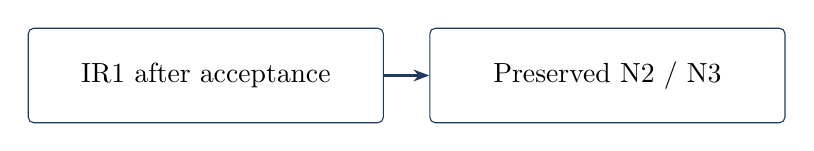
\begin{tikzpicture}[y=.70cm]
\node[box,font=\normalsize,text width=43mm,minimum height=12mm] (a0) at (0.0,0) {IR1 after acceptance};
\node[box,font=\normalsize,text width=43mm,minimum height=12mm] (a1) at (5.1,0) {Preserved N2 / N3};
\draw[flow] (a0.east) -- (a1.west);\end{tikzpicture}\par\medskip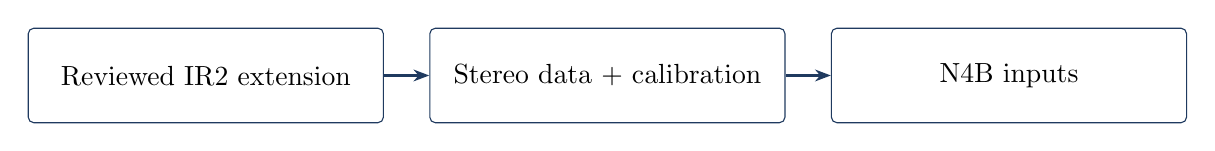
\begin{tikzpicture}[y=.70cm]
\node[box,font=\normalsize,text width=43mm,minimum height=12mm] (a0) at (0.0,0) {Reviewed IR2 extension};
\node[box,font=\normalsize,text width=43mm,minimum height=12mm] (a1) at (5.1,0) {Stereo data + calibration};
\draw[flow] (a0.east) -- (a1.west);
\node[box,font=\normalsize,text width=43mm,minimum height=12mm] (a2) at (10.2,0) {N4B inputs};
\draw[flow] (a1.east) -- (a2.west);\end{tikzpicture}}{Stereo extension; schematic.}
\vfill\takeaway{The stereo goal does not authorize quietly changing N2.}
\note{Backup group: Gate acceptance and diagnosis. Latest status: experiments/2026-10-14-SESSION\_FACTS\_ADDENDUM.md. An IR1-only dataset cannot feed stereo-inertial estimation. Prepare a separately reviewed extension with both camera projections, stereo extrinsics/rectification, all required motion/time coverage, explicit topics and lossless data. Existing mono-inertial candidate artifacts are not stereo qualification. Source register: B,G,O. PLANNED separately reviewed IR2 profile/topic/storage/calibration extension precedes N4B; accepted IR1-only N2/N3 stay intact.}\end{frame}
\begin{frame}{Backup: 4.9 N4A: estimator acceptance contract}\evidence{PLANNED / no gate PASS}
Absolute Trajectory Error (ATE) scores aligned paths; Relative Pose Error (RPE) scores motion increments.\par\medskip\begin{tabular}{@{}L{80mm}L{104mm}@{}}\toprule
\textbf{Required / open threshold} & \textbf{Measurement / clock}\\\midrule
Finite ordered trajectories; coverage & Export epochs in dataset time; coordinate/format audit\\[6pt]
Repeat initialization / tracking & All attempts incl. failure; first eligible dataset epoch + host events\\[6pt]
Accuracy / continuity budgets UNKNOWN & Reference association, rigid alignment, ATE/RPE; dataset epochs\\[6pt]
\bottomrule\end{tabular}\par\medskip FAIL: load/link error $\to$ build; empty images $\to$ reader paths; no inertial initialization $\to$ settings/time/motion. No accepted numeric budget means no performance PASS. N4A RPE is unverified in Phase-8 permitted sources; stable-power reruns and reviewed budgets remain missing.\vfill\takeaway{MH01 accuracy is measured; N0 power health and this contract remain incomplete.}\note{Backup group: Gate acceptance and diagnosis. Latest status: experiments/2026-10-14-SESSION\_FACTS\_ADDENDUM.md. Source: docs/ORB\_SLAM3\_OFFLINE\_PREPARATION.md; upstream pinned stereo\_inertial\_euroc.cc. Commands are teaching examples only; none executed. UNKNOWN budgets require approval. Original evidence table (thresholds unchanged): \begin{tabular}{@{}L{65mm}L{77mm}L{38mm}@{}}\toprule
\textbf{Required / open threshold} & \textbf{Measurement / clock} & \textbf{Proposed evidence}\\\midrule
Finite ordered trajectories; coverage & Export epochs in dataset time; coordinate/format audit & Trajectory files + audit\\[6pt]
Repeat initialization / tracking & All attempts incl. failure; first eligible dataset epoch + host events & Run/state timelines\\[6pt]
Accuracy / continuity budgets UNKNOWN & Reference association, rigid alignment, ATE/RPE; dataset epochs & evo outputs + budget review\\[6pt]
\bottomrule\end{tabular}}\end{frame}
\begin{frame}{Backup: 4.10 N4B: input and run criteria}\evidence{PLANNED / no gate PASS}
\par\begin{tabular}{@{}L{80mm}L{104mm}@{}}\toprule
\textbf{Required / open threshold} & \textbf{Measurement / clock}\\\midrule
Lossless stereo + valid pairing & Counts/pixels, epipolar residuals, left/right stamp difference; source domain\\[6pt]
Calibrated geometry, noise and offset & Holdout residuals; camera/IMU units and common time relation\\[6pt]
Repeatable finite tracking; budgets UNKNOWN & All trials, epochs, initialization/loss; no GT means accuracy UNKNOWN\\[6pt]
\bottomrule\end{tabular}\par\medskip FAIL: vertical mismatch $\to$ rectification; missing brackets $\to$ motion coverage; bias instability $\to$ clocks/calibration before feature tuning. Residual limits are not yet approved.\vfill\takeaway{Factory nominal geometry and assumed numeric noise do not qualify final VIO.}\note{Backup group: Gate acceptance and diagnosis. Latest status: experiments/2026-10-14-SESSION\_FACTS\_ADDENDUM.md. Source: docs/ORB\_SLAM3\_OFFLINE\_PREPARATION.md; upstream pinned stereo\_inertial\_euroc.cc. Commands are teaching examples only; none executed. UNKNOWN budgets require approval. Original evidence table (thresholds unchanged): \begin{tabular}{@{}L{63mm}L{79mm}L{38mm}@{}}\toprule
\textbf{Required / open threshold} & \textbf{Measurement / clock} & \textbf{Proposed evidence}\\\midrule
Lossless stereo + valid pairing & Counts/pixels, epipolar residuals, left/right stamp difference; source domain & Association / image audit\\[6pt]
Calibrated geometry, noise and offset & Holdout residuals; camera/IMU units and common time relation & Calibration report + hashes\\[6pt]
Repeatable finite tracking; budgets UNKNOWN & All trials, epochs, initialization/loss; no GT means accuracy UNKNOWN & Run logs + trajectories\\[6pt]
\bottomrule\end{tabular}}\end{frame}
\begin{frame}{Backup: 4.10 N4B: immutable adapter provenance}\evidence{MEASURED binary build / replay OPEN}
\begin{columns}[T,onlytextwidth]\begin{column}{.48\textwidth}\begin{block}{Derived input contract}Preserve raw bags. Manifest links input, converter, settings and calibration hashes; record domains, offset sign, interpolation brackets and every rejected sample.\end{block}\end{column}\begin{column}{.48\textwidth}\coursefigure{P10}{\slideimg[.46\textheight]{\linewidth}{P10}{Offline frozen-input analysis}}{Frozen inputs make estimator comparisons attributable.}\end{column}\end{columns}\vfill\takeaway{In Figure~\ref{fig:P10}, test lossless pixels, exact nanoseconds, no extrapolation and count reconciliation.}\note{Backup group: Gate acceptance and diagnosis. Latest status: experiments/2026-10-14-SESSION\_FACTS\_ADDENDUM.md. Source: docs/ORB\_SLAM3\_OFFLINE\_PREPARATION.md; upstream pinned stereo\_inertial\_euroc.cc. Commands are teaching examples only; none executed. UNKNOWN budgets require approval.}\end{frame}
\begin{frame}{Backup: 4.11 N4C: live PASS/FAIL criteria}\evidence{PLANNED / no gate PASS}
\par\begin{tabular}{@{}L{80mm}L{104mm}@{}}\toprule
\textbf{Required / open threshold} & \textbf{Measurement / clock}\\\midrule
Valid paired input + IMU coverage & Source epochs; renewed stereo transport metrics\\[6pt]
Initialization / continuity budgets UNKNOWN & Attempt count; loss/reset state; source epochs + host event times\\[6pt]
Latency / queue bounds UNKNOWN & Queue, compute, receipt/output on host steady; mapped capture with uncertainty\\[6pt]
\bottomrule\end{tabular}\par\medskip FAIL: offline works, live lags $\to$ SDK callback/queue in the direct path; ROS delivery in the planned path; thermal stalls $\to$ N0 under load; loss in both $\to$ input/calibration first. Missing counters stay UNKNOWN.\vfill\takeaway{Approve bounds before a live performance verdict; do not tune around unmeasured age.}\note{Backup group: Gate acceptance and diagnosis. Latest status: experiments/2026-10-14-SESSION\_FACTS\_ADDENDUM.md. Source: docs/ORB\_SLAM3\_OFFLINE\_PREPARATION.md; upstream pinned stereo\_inertial\_euroc.cc. Commands are teaching examples only; none executed. UNKNOWN budgets require approval. Original evidence table (thresholds unchanged): \begin{tabular}{@{}L{65mm}L{77mm}L{38mm}@{}}\toprule
\textbf{Required / open threshold} & \textbf{Measurement / clock} & \textbf{Proposed evidence}\\\midrule
Valid paired input + IMU coverage & Source epochs; renewed stereo transport metrics & Input / pairing timeline\\[6pt]
Initialization / continuity budgets UNKNOWN & Attempt count; loss/reset state; source epochs + host event times & State timeline / trajectories\\[6pt]
Latency / queue bounds UNKNOWN & Queue, compute, receipt/output on host steady; mapped capture with uncertainty & Latency / queue / health log\\[6pt]
\bottomrule\end{tabular}}\end{frame}
\begin{frame}{Backup: 4.12 N5: measurement criteria}\evidence{PLANNED / no gate PASS}
\par\begin{tabular}{@{}L{80mm}L{104mm}@{}}\toprule
\textbf{Required / open threshold} & \textbf{Measurement / clock}\\\midrule
ATE/RPE only with valid reference & Associated source epochs; rigid alignment; overlap and exclusions\\[6pt]
P50/P95/P99 + initialization/loss & Named interval, estimator and sample count; host steady / source epochs\\[6pt]
Resources, losses, queue depth & One-Hz health + event join; sequence/count reconciliation; unknown counters marked\\[6pt]
\bottomrule\end{tabular}\par\medskip All numeric performance budgets are UNKNOWN. FAIL: cross-domain subtraction $\to$ clocks; suspicious low ATE $\to$ alignment/association; averages hide stalls $\to$ raw timeline.\par\medskip\textbf{Continuity denominator}: Count all initialization attempts; define first eligible input. Record state, reset/session ID, loss intervals and trajectory coverage.\par\vfill\takeaway{Missing ground truth blocks accuracy claims; it does not force synthetic zero errors.}\note{Backup group: Gate acceptance and diagnosis. Latest status: experiments/2026-10-14-SESSION\_FACTS\_ADDENDUM.md. Source: docs/ORB\_SLAM3\_OFFLINE\_PREPARATION.md; upstream pinned stereo\_inertial\_euroc.cc. Commands are teaching examples only; none executed. UNKNOWN budgets require approval. Merged original page 93: 
\deckitems{\item Success rate uses all declared initialization attempts as denominator.\item Measure initialization time from a defined first eligible input.\item Track loss duration, resets and relocalization events.\item Check trajectory coverage, not only exported sample count.}
\vfill
\begin{tabular}{L{87.0mm}L{87.0mm}}\toprule
\textbf{Event record} & \textbf{Required interpretation}\\\midrule
First eligible input & Initialization-time origin\\[5pt]
Tracking state / reset & Continuity and loss intervals\\[5pt]
Pose epoch / output time & Coverage versus freshness\\[5pt]
\bottomrule\end{tabular}
\vfill\takeaway{Report failed attempts alongside successful trajectories.}
Retain sensor epoch, local event time, state, reset/session/map identifier and exclusion reason. Pose export presence alone cannot recover all state events. Numerical state-event instrumentation and interface changes require review before implementation. Source register: O,U. Success denominator, initialization time, tracking loss duration, resets and relocalization need preserved state events and failed trials. Original evidence table (thresholds unchanged): \begin{tabular}{@{}L{61mm}L{79mm}L{40mm}@{}}\toprule
\textbf{Required / open threshold} & \textbf{Measurement / clock} & \textbf{Proposed evidence}\\\midrule
ATE/RPE only with valid reference & Associated source epochs; rigid alignment; overlap and exclusions & evo raw output / audit\\[6pt]
P50/P95/P99 + initialization/loss & Named interval, estimator and sample count; host steady / source epochs & Raw events + trial summary\\[6pt]
Resources, losses, queue depth & One-Hz health + event join; sequence/count reconciliation; unknown counters marked & Health / counter time series\\[6pt]
\bottomrule\end{tabular} Consolidated audit BACKUP 66: \textbf{4.12 N5: reproducible measurement}\evidence{PLANNED / no gate PASS}
Entry: qualified N4 trials, frozen hypotheses, trial count, reference and clock relations. Retain failures; at least three offline repeats is a PLANNED minimum.\begin{block}{Future commands / tools}{\ttfamily\normalsize evo\_ape tum REFERENCE.tum ESTIMATE.tum --align\par evo\_rpe tum REFERENCE.tum ESTIMATE.tum --help}\end{block}\begin{columns}[T,onlytextwidth]\begin{column}{.48\textwidth}\begin{block}{Outputs}Original exports, conversion audit, evo version/argv/results, latency samples with eligibility, initialization/loss events and resource time series.\end{block}\end{column}\begin{column}{.48\textwidth}\begin{block}{Tools still planned}Event instrumentation and queue counters need reviewed implementation. No first-party N5 acceptance validator exists. Approve metric bounds before the campaign.\end{block}\end{column}\end{columns}\vfill\takeaway{A metric file is a measurement artifact, not automatic performance acceptance.}Source: docs/ORB\_SLAM3\_OFFLINE\_PREPARATION.md; upstream pinned stereo\_inertial\_euroc.cc; evo maintainer Metrics [8]. Commands are teaching examples only; none executed. UNKNOWN budgets require approval.}\end{frame}
% BACKUP GROUP: ROS communication and transforms
\begin{frame}{Backup: 2.6 QoS compatibility}\evidence{KNOWN ROS semantics}
\deckitems{\item Quality of Service (QoS) is an offered/requested contract. \hyperlink{referencepage}{[3]} \item A reliable reader cannot match a best-effort-only writer.\item Sensor observers use best-effort, volatile subscriptions.\item Static transforms use reliable, transient-local delivery.}
\vfill
\begin{tabular}{L{56.666666666666664mm}L{56.666666666666664mm}L{56.666666666666664mm}}\toprule
\textbf{Writer} & \textbf{Reader} & \textbf{Compatible}\\\midrule
Best effort & Reliable & No\\[5pt]
Reliable & Best effort & Yes\\[5pt]
Volatile & Transient local & No\\[5pt]
\bottomrule\end{tabular}
\vfill\takeaway{Topic names alone cannot prove a compatible connection.}
\note{Backup group: ROS communication and transforms. Latest status: experiments/2026-10-14-SESSION\_FACTS\_ADDENDUM.md. Inspect reliability, durability, history/depth, deadline and lifespan where relevant. Reliable writers can satisfy best-effort readers. A volatile writer cannot satisfy a transient-local reader. Latched context must reach recorder and replay observer. Source register: Q. Quality of Service (QoS) compatibility is offered/requested; reliable subscription cannot consume best-effort-only publication.}\end{frame}
\begin{frame}{Backup: 3.4 Topic and type contract}\evidence{PLANNED / no gate PASS}
\par\begin{tabular}{@{}L{73mm}L{69mm}L{38mm}@{}}\toprule
\textbf{Topic below /camera/camera} & \textbf{Message / cadence} & \textbf{Reader policy}\\\midrule
\texttt{infra1/image\_rect\_raw} & \texttt{sensor\_msgs/msg/Image}; 15 Hz & Best effort / volatile\\[6pt]
\texttt{infra1/camera\_info} & \texttt{sensor\_msgs/msg/CameraInfo}; 15 Hz & Best effort / volatile\\[6pt]
\texttt{gyro/sample}; \texttt{accel/sample} & \texttt{sensor\_msgs/msg/Imu}; 200 / 100 Hz & Best effort / volatile\\[6pt]
\texttt{/tf\_static} (absolute topic) & \texttt{tf2\_msgs/msg/TFMessage}; static & Reliable / transient local\\[6pt]
\bottomrule\end{tabular}\par\vfill\takeaway{Rates are requested baseline values; verify offers, depth and actual delivery.}\note{Backup group: ROS communication and transforms. Latest status: experiments/2026-10-14-SESSION\_FACTS\_ADDENDUM.md. Source: experiments/2026-09-12-pi5-native-sensor-validation/PHASE\_A\_RUNBOOK.md; n3\_topics.json; ROS Jazzy QoS [3]. Commands are teaching examples only; none executed. UNKNOWN budgets require approval.}\end{frame}
\begin{frame}{Backup: 3.11 Robot transform ownership}\evidence{PLANNED / no gate PASS}
\par\medskip\coursefigure{D27}{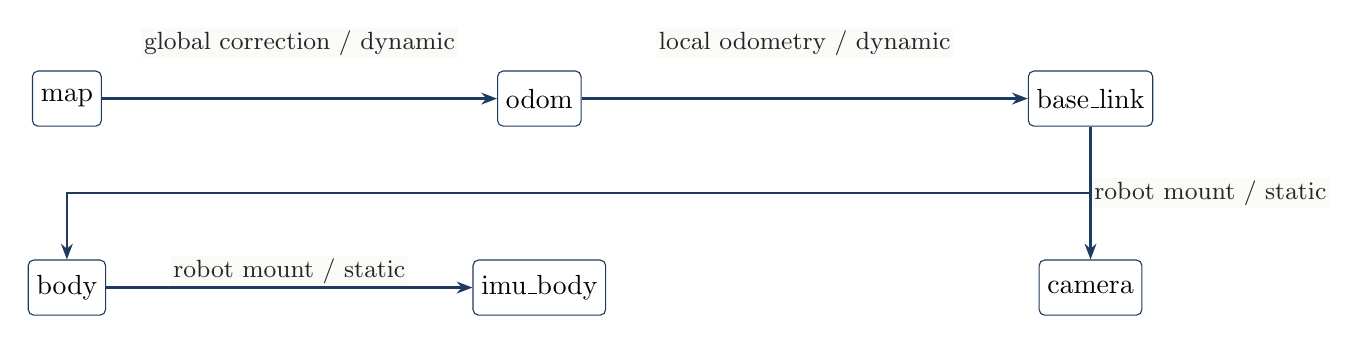
\begin{tikzpicture}[y=.8cm,font=\normalsize,box/.append style={font=\normalsize}]
\node[box] (map) at (0,0) {map};\node[box] (odom) at (6,0) {odom};\node[box] (base) at (13,0) {base\_link};
\draw[flow] (map)--node[above=5mm,lbl]{global correction / dynamic}(odom);
\draw[flow] (odom)--node[above=5mm,lbl]{local odometry / dynamic}(base);
\node[box] (body) at (0,-3) {body};\node[box] (imu) at (6,-3) {imu\_body};\node[box] (cam) at (13,-3) {camera};
\draw[flow] (base.south)--(13,-1.5)--(0,-1.5)--(body.north);
\draw[flow] (body)--node[above,lbl]{robot mount / static}(imu);
\draw[flow] (base)--node[right,lbl]{robot mount / static}(cam);
\end{tikzpicture}}{Dynamic edges need separate planned estimator and continuity owners.}\par\medskip Robot description owns static mounts, including base\_link $\to$ body. The planned bridge owns dynamic edges; implementation is UNKNOWN. Optional world $\to$ map needs an explicit external-reference owner [4].\vfill\takeaway{In Figure~\ref{fig:D27}, one parent and one publisher per child; never relabel a jumping map pose as odom.}\note{Backup group: ROS communication and transforms. Latest status: experiments/2026-10-14-SESSION\_FACTS\_ADDENDUM.md. Source: docs/ARCHITECTURE.md; REP-103/105. Commands are teaching examples only; none executed. UNKNOWN budgets require approval.}\end{frame}
\begin{frame}{Backup: 3.12 Camera transform ownership}\evidence{PLANNED / no gate PASS}
\par\medskip\coursefigure{D28}{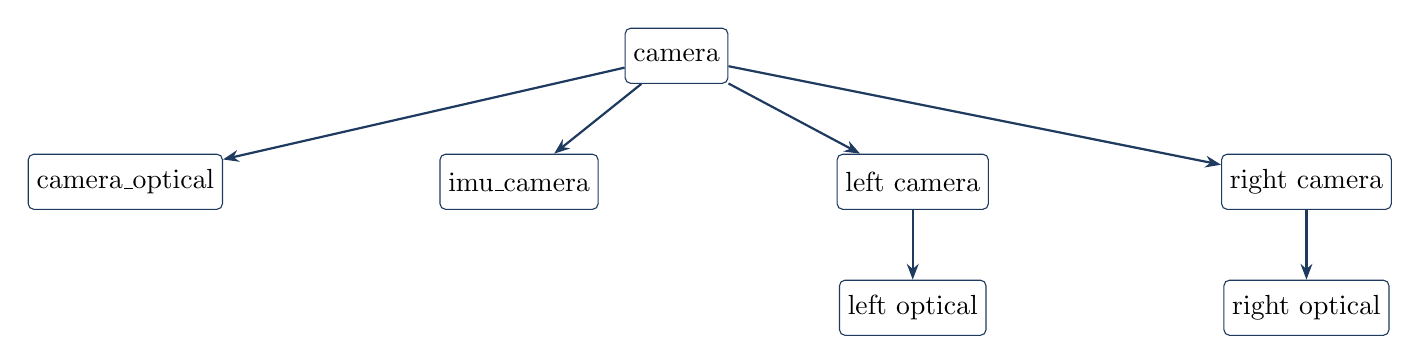
\begin{tikzpicture}[y=.8cm,font=\normalsize,box/.append style={font=\normalsize}]
\node[box] (cam) at (7,0) {camera};
\node[box] (opt) at (0,-2) {camera\_optical};\node[box] (imu) at (5,-2) {imu\_camera};
\node[box] (left) at (10,-2) {left camera};\node[box] (right) at (15,-2) {right camera};
\foreach \n in {opt,imu,left,right}{\draw[flow] (cam)--(\n);}
\node[box] (lo) at (10,-4) {left optical};\node[box] (ro) at (15,-4) {right optical};
\draw[flow] (left)--(lo);\draw[flow] (right)--(ro);
\end{tikzpicture}}{Wrapper-owned sensor geometry is static; frame names here are conceptual.}\par\medskip Wrapper /camera/camera publishes sensor edges on /tf\_static when tf\_publish\_rate=0. Inspect actual parents and frame IDs; do not add this conceptual tree as a second publisher.\vfill\takeaway{In Figure~\ref{fig:D28}, the robot description owns the camera mount; the wrapper owns internal sensor geometry.}\note{Backup group: ROS communication and transforms. Latest status: experiments/2026-10-14-SESSION\_FACTS\_ADDENDUM.md. Source: experiments/2026-09-12-pi5-native-sensor-validation/PHASE\_A\_RUNBOOK.md; n3\_baseline.yaml. Commands are teaching examples only; none executed. UNKNOWN budgets require approval.}\end{frame}
\begin{frame}{Backup: 3.16 Where timestamps are stamped}\evidence{PLANNED / no gate PASS}
\par\begin{tabular}{@{}L{43mm}L{55mm}L{82mm}@{}}\toprule
\textbf{Field / event} & \textbf{Stamp owner} & \textbf{Interpretation}\\\midrule
$t_{dev}$ / sensor frame & Device + SDK metadata & Hardware-relative or mapped domain; inspect each frame\\[6pt]
$t_{hdr}$ / message header & ROS wrapper & Producer epoch; not publish time\\[6pt]
$t_{rx},t_s,t_e,t_o$ & Observer / adapter instrumentation & Local steady-clock receipt, start, end, emission\\[6pt]
$t_{bag}$ / storage record & rosbag2 / storage backend & Recorder time; never substitute for source header\\[6pt]
\bottomrule\end{tabular}\par\vfill\takeaway{A trajectory stamp is the estimated pose epoch, not when its file was written.}\note{Backup group: ROS communication and transforms. Latest status: experiments/2026-10-14-SESSION\_FACTS\_ADDENDUM.md. Source: experiments/2026-09-12-pi5-native-sensor-validation/PHASE\_A\_RUNBOOK.md; n3\_metrics.py. Commands are teaching examples only; none executed. UNKNOWN budgets require approval.}\end{frame}
\begin{frame}{Backup: 3.17 Global time}\evidence{PLANNED}
\deckitems{\item Global-time option readback is a configuration observation. \hyperlink{referencepage}{[5]} \item The SDK maps device time toward host time.\item Enabled global time does not measure camera–IMU offset.\item Arrival minus mapped stamp is not pure USB latency.}
\vfill
\begin{tabular}{L{87.0mm}L{87.0mm}}\toprule
\textbf{Observation} & \textbf{What it establishes}\\\midrule
Option enabled & Requested timestamp behavior\\[5pt]
Frame domain & Per-frame clock classification\\[5pt]
Mapped timestamp & Relationship with mapping uncertainty\\[5pt]
Camera–IMU offset & Separate physical alignment measurement\\[5pt]
\bottomrule\end{tabular}
\vfill\takeaway{Record domains and uncertainty before reporting source age.}
\note{Backup group: ROS communication and transforms. Latest status: experiments/2026-10-14-SESSION\_FACTS\_ADDENDUM.md. Pinned v2.58.4 global\_timestamp\_reader.cpp provides algorithm evidence. Historical metadata read global time 1, but actual frame domains were not measured in that session. Off/on diagnostics must use separate labeled runs and preserve raw stamps. Source register: C,CLK. Enabled global-time option is not measured camera–IMU offset or pure USB latency.}\end{frame}
\begin{frame}{Backup: 3.18 Worked latency decomposition}\evidence{PLANNED / no gate PASS}
\par\medskip\coursefigure{D34}{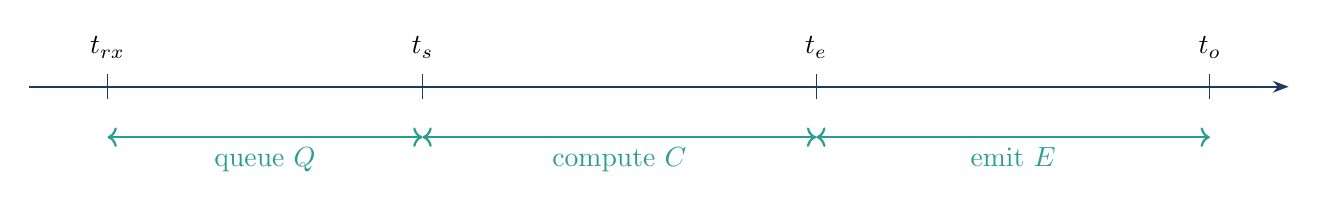
\begin{tikzpicture}[y=.8cm,font=\normalsize,box/.append style={font=\normalsize}]
\draw[flow] (0,0)--(16,0);
\foreach \x/\t in {1/$t_{rx}$,5/$t_s$,10/$t_e$,15/$t_o$}{\draw[navy] (\x,-.2)--(\x,.2);\node[above] at (\x,.3){\t};}
\draw[<->,teal,thick] (1,-.8)--node[below]{queue $Q$}(5,-.8);
\draw[<->,teal,thick] (5,-.8)--node[below]{compute $C$}(10,-.8);
\draw[<->,teal,thick] (10,-.8)--node[below]{emit $E$}(15,-.8);
\end{tikzpicture}}{All three components use the same host steady clock.}\par\medskip $L_{rx\to o}=(t_s-t_{rx})+(t_e-t_s)+(t_o-t_e)=Q+C+E$.\par\medskip Capture age requires $\widehat t_c=g(t_{dev})$ in this domain. If mapping error is bounded by $u$, true age lies in $[t_o-\widehat t_c-u,\ t_o-\widehat t_c+u]$.\vfill\takeaway{In Figure~\ref{fig:D34}, fast compute does not imply fresh output when queue wait dominates.}\note{Backup group: ROS communication and transforms. Latest status: experiments/2026-10-14-SESSION\_FACTS\_ADDENDUM.md. Source: experiments/2026-09-12-pi5-native-sensor-validation/PHASE\_A\_RUNBOOK.md. Commands are teaching examples only; none executed. UNKNOWN budgets require approval.}\end{frame}
% BACKUP GROUP: Configuration and calibration
\begin{frame}{Backup: 3.22 IMU noise}\evidence{PLANNED}
\deckitems{\item Allan deviation compares noise across averaging time $\tau$. \hyperlink{referencepage}{[7]}  (Figure~\ref{fig:D38})\item Short-time slope helps estimate white-noise density.\item Longer records are needed to constrain bias instability or walk.\item Vendor comma-separated values (CSV) round motion; use full precision.}
\vfill
\coursefigure{D38}{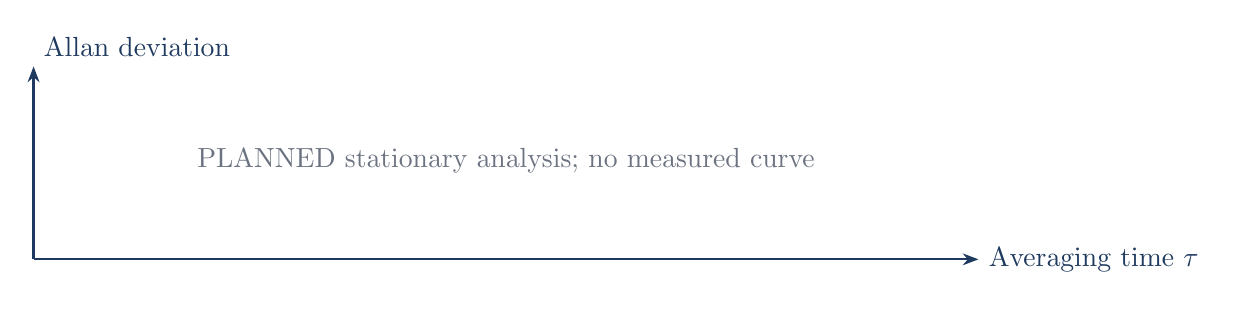
\begin{tikzpicture}[font=\normalsize,y=.70cm]
\draw[flow] (0,0)--(12,0) node[right]{Averaging time $\tau$};\draw[flow] (0,0)--(0,3.5) node[above right]{Allan deviation};
\node[text=muted] at (6,1.8) {PLANNED stationary analysis; no measured curve};\end{tikzpicture}}{IMU noise; schematic.}
\vfill\takeaway{Choose stationary duration from the averaging times you need.}
\note{Backup group: Configuration and calibration. Latest status: experiments/2026-10-14-SESSION\_FACTS\_ADDENDUM.md. Allan variance is half the mean squared difference between adjacent interval averages; Allan deviation is its square root. Record sample units/rates, temperature, stationary validity and confidence/sample support. Do not confuse bias instability with random walk. Tool compatibility and unit-specific parameters remain unknown. Source register: C,I. Allan variance/deviation separates noise and bias across averaging times; long enough full-precision stationary input is required.}\end{frame}
\begin{frame}{Backup: 3.28 Settings audit before tuning}\evidence{PLANNED / no gate PASS}
\par\begin{tabular}{@{}L{48mm}L{85mm}L{47mm}@{}}\toprule
\textbf{Pinned parser group} & \textbf{Meaning / check} & \textbf{Failure implication}\\\midrule
Camera1 / Camera2; Stereo & Projection, distortion, b or T\_c1\_c2; selected rectification path & Wrong disparity geometry; scale / epipolar error\\[6pt]
IMU.T\_b\_c1 & Camera $\to$ estimator IMU; numeric basis-vector / inverse test & Axis/sign error; gravity or bias inconsistency\\[6pt]
IMU.Frequency; four noise fields & Continuous-time densities / walks; discretize once & False confidence; unstable initialization\\[6pt]
ORBextractor fields & Feature count, pyramid, FAST thresholds & Tune only after input, timing and calibration\\[6pt]
\bottomrule\end{tabular}\par\vfill\takeaway{The active stereo candidate uses nominal geometry and assumed noise; qualification remains OPEN.}\note{Backup group: Configuration and calibration. Latest status: experiments/2026-10-14-SESSION\_FACTS\_ADDENDUM.md. Source: docs/ORB\_SLAM3\_OFFLINE\_PREPARATION.md; upstream pinned stereo\_inertial\_euroc.cc. Commands are teaching examples only; none executed. UNKNOWN budgets require approval. Consolidated audit BACKUP 23: \textbf{3.14 Transform direction}\evidence{KNOWN source convention / PLANNED tests}
\deckitems{\item Camera-to-estimator-IMU transform: $p_b=T_{b\_c1}p_c$. (Figure~\ref{fig:D30})\item Its inverse maps IMU coordinates back into the camera.\item SDK rotation arrays and OpenCV matrix storage orders differ.\item Test basis vectors, inversion and composition.}
\vfill
\coursefigure{D30}{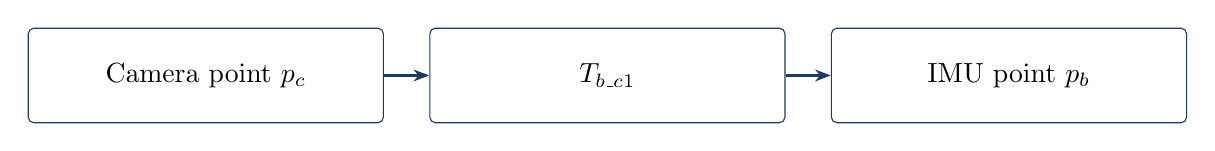
\begin{tikzpicture}[y=.70cm]
\node[box,font=\normalsize,text width=43mm,minimum height=12mm] (a0) at (0.0,0) {Camera point $p_c$};
\node[box,font=\normalsize,text width=43mm,minimum height=12mm] (a1) at (5.1,0) {$T_{b\_c1}$};
\draw[flow] (a0.east) -- (a1.west);
\node[box,font=\normalsize,text width=43mm,minimum height=12mm] (a2) at (10.2,0) {IMU point $p_b$};
\draw[flow] (a1.east) -- (a2.west);\end{tikzpicture}}{Transform direction; schematic.}
\vfill\takeaway{Transform direction must follow code and numeric tests.}
Frame.cc composes T\_cb with T\_bw; ImuTypes.cc stores T\_cb = inverse(T\_bc). SDK rotations are column-major; OpenCV YAML data are row-major. b here denotes estimator IMU/body, never automatically robot body. Identity defaults do not validate a future nonidentity calibration. Source register: C,O,U. p\_b = T\_b\_c1 p\_c; test inverse/basis vectors and column-major SDK versus row-major OpenCV arrays.}\end{frame}
\begin{frame}{Backup: 3.28 Numeric IMU settings contract}\evidence{PLANNED / no gate PASS}
YAML (YAML Ain’t Markup Language) settings must follow the selected pinned parser. Unit-specific noise is UNKNOWN; the diagnostic candidate uses ASSUMED upstream numeric values.\par\begin{tabular}{@{}L{73mm}L{111mm}@{}}\toprule
\textbf{Key family} & \textbf{Interpretation}\\\midrule
IMU.NoiseGyro / NoiseAcc & Continuous-time gyro / accel noise densities; code multiplies by $\sqrt{f}$\\[6pt]
IMU.GyroWalk / AccWalk & Bias random-walk quantities; code divides by $\sqrt{f}$\\[6pt]
IMU.Frequency / T\_b\_c1 & Input-grid frequency $f$ / camera-to-IMU transform; not raw accel rate\\[6pt]
\bottomrule\end{tabular}\par\medskip Camera.width/height/fps and Camera1/Camera2 keys must match actual inputs. Example EuRoC values describe that dataset; they are not D435i calibration.\vfill\takeaway{Do not discretize densities twice; assumed upstream values enable diagnostics, not qualification.}\note{Backup group: Configuration and calibration. Latest status: experiments/2026-10-14-SESSION\_FACTS\_ADDENDUM.md. Source: docs/ORB\_SLAM3\_OFFLINE\_PREPARATION.md; upstream pinned stereo\_inertial\_euroc.cc. Commands are teaching examples only; none executed. UNKNOWN budgets require approval.}\end{frame}
\begin{frame}{Backup: 3.29 Input association}\evidence{PREPARED helper / runtime association UNVERIFIED}
\deckitems{\item Prepared helper interpolates accel only between valid brackets. (Figure~\ref{fig:D45})\item Use gyro epochs for a reviewed combined input grid.\item Reject gaps, duplicate/backward time and extrapolation.\item Retain originals and every interpolation/rejection decision.}
\vfill
\coursefigure{D45}{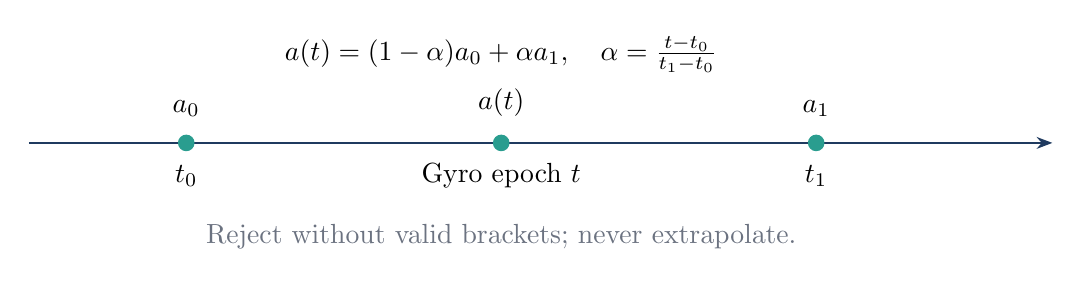
\begin{tikzpicture}[font=\normalsize,y=.70cm]
\draw[flow] (0,0)--(13,0);\foreach \x in {2,6,10}{\fill[teal] (\x,0) circle (3pt);}\node[above] at (2,.3){$a_0$};\node[above] at (6,.3){$a(t)$};\node[above] at (10,.3){$a_1$};
\node at (2,-.6){$t_0$};\node at (6,-.6){Gyro epoch $t$};\node at (10,-.6){$t_1$};
\node at (6,1.6){$a(t)=(1-\alpha)a_0+\alpha a_1,\quad \alpha=\frac{t-t_0}{t_1-t_0}$};
\node[text=muted] at (6,-1.7){Reject without valid brackets; never extrapolate.};\end{tikzpicture}}{Input association; schematic.}
\vfill\takeaway{A 200 Hz input grid does not make raw accel 200 Hz.}
\note{Backup group: Configuration and calibration. Latest status: experiments/2026-10-14-SESSION\_FACTS\_ADDENDUM.md. Current helper source: experiments/2026-10-13-n4b-d435i-prep/d435i\_input.h and verification.md (offline/synthetic); Pi build status: experiments/2026-10-13-SESSION\_FACTS\_FOR\_SLIDES.md, section E. Diagnostic stream recordings now exist; complete association/rejection behavior remains unverified. a(t) = (1−$\alpha$)a0 + $\alpha$a1 with $\alpha$=(t−t0)/(t1−t0), t0$\leq$t$\leq$t1. Verify known linear signals, irregular spacing, missing endpoints and exact nanosecond conversions. Apply measured time offset once with a tested sign. A candidate mono adapter is not an implemented stereo input path. Source register: O,C. PLANNED accel interpolation on gyro times requires bracketing/gap rejection/no extrapolation; 200 Hz combined input is not 200 Hz raw accel.}\end{frame}
% BACKUP GROUP: Metrics and resource questions
\begin{frame}{Backup: 5.2 ATE computation outline}\evidence{PLANNED / no gate PASS}
Absolute Trajectory Error (ATE) compares associated poses after a declared alignment. $P_i$ is the estimate and $Q_i$ the reference; root mean square error (RMSE) summarizes translation [8].\par\medskip\coursefigure{D70}{
\begin{tikzpicture}[y=.8cm,font=\normalsize,box/.append style={font=\normalsize}]\node[box,text width=165mm] {$E_i=Q_i^{-1}SP_i,\qquad e_i=\|\operatorname{trans}(E_i)\|,\qquad \mathrm{RMSE}=\sqrt{\frac{1}{N}\sum_i e_i^2}$};\end{tikzpicture}}{Rigid alignment S removes reference-origin choice, not a stereo scale error.}\par\medskip Associate epochs within a predeclared tolerance; retain unmatched samples. Convert both trajectories to the same pose direction and units before fitting $S$. Report valid overlap and failure trials.\vfill\takeaway{In Figure~\ref{fig:D70}, without independent reference data, D435i absolute accuracy stays UNKNOWN.}\note{Backup group: Metrics and resource questions. Latest status: experiments/2026-10-14-SESSION\_FACTS\_ADDENDUM.md. Source: docs/ORB\_SLAM3\_OFFLINE\_PREPARATION.md; upstream pinned stereo\_inertial\_euroc.cc; evo Metrics. Commands are teaching examples only; none executed. UNKNOWN budgets require approval.}\end{frame}
\begin{frame}{Backup: 5.3 RPE and pair policy}\evidence{RPE UNVERIFIED in permitted sources / no gate PASS}
Relative Pose Error (RPE) compares estimated motion with reference motion over a declared interval [8].\par\medskip\coursefigure{D71}{
\begin{tikzpicture}[y=.8cm,font=\normalsize,box/.append style={font=\normalsize}]\node[box,text width=165mm] {$E_{ij}=(Q_i^{-1}Q_j)^{-1}(P_i^{-1}P_j)$\\Translation and rotation are separate metrics.};\end{tikzpicture}}{Relative deltas expose local drift rather than global alignment choice.}\par\par\begin{tabular}{@{}L{83mm}L{101mm}@{}}\toprule
\textbf{Pair policy} & \textbf{Question answered}\\\midrule
Fixed time separation & How wrong is motion over that duration?\\[6pt]
Fixed distance separation & How does error grow per traveled distance?\\[6pt]
Consecutive vs all eligible pairs & Different weighting; report choice and pair count\\[6pt]
\bottomrule\end{tabular}\par\vfill\takeaway{In Figure~\ref{fig:D71}, never compare RPE numbers with different delta units or pairing policies.}\note{Backup group: Metrics and resource questions. Latest status: experiments/2026-10-14-SESSION\_FACTS\_ADDENDUM.md. Phase-8 audit: earlier RPE calculation is UNVERIFIED IN PERMITTED SOURCES; source backup preserves its original exact values and provenance. Earlier claim, not adopted as current fact: Evidence: slides\_course/qa/n4a-traj-eval-summary.md; tools/trajectory\_eval/README.md. CALCULATED using traj\_eval.py from claude/project-thread-upkfjv, commit d3f9540, PR 2; tool not yet merged. Earlier Phase-7 claim: tool validation passed per its README, not rerun by this deck task. Flags: --t-max-diff 0.02 --t-offset 0 --align-both --rotation-ate --rpe-delta 1 --rpe-unit s. Shared EuRoC clock assumed; offset zero; active body-to-world poses in imu\_body, metres. 3,639 timestamp-associated pose pairs per run. For each eligible start, choose the first later reference timestamp at least 1 s later; no interpolation. SE(3) rigid alignment cancels in RPE. The tool's SE(3) ATE reproduces saved evo scores; its RPE pair policy differs from evo filters. Sim(3) additionally fits scale and is diagnostic, not the stereo-inertial paper comparator. Does not establish frames, extrinsics, synchronization, sensor readiness or gate PASS. No new camera, Pi or ORB execution. Source: evo Metrics [8]. Commands are teaching examples only; none executed. UNKNOWN budgets require approval.}\end{frame}
\begin{frame}{Backup: 5.6 Latency and loss}\evidence{PLANNED}
\deckitems{\item P50/P95/P99 are the 50th/95th/99th latency percentiles.\item Name receipt-to-start, processing and receipt-to-output separately.\item Reconcile sequence gaps, received counts and recorded counts.\item Unavailable queue/drop counters remain UNKNOWN.}
\vfill
\begin{tabular}{L{87.0mm}L{87.0mm}}\toprule
\textbf{Metric} & \textbf{Required evidence}\\\midrule
Latency percentiles & Named interval / clock / count\\[5pt]
Loss & Sequence and count reconciliation\\[5pt]
Queue depth / drops & Measured counter or UNKNOWN\\[5pt]
\bottomrule\end{tabular}
\vfill\takeaway{Percentiles need event definitions and eligible sample counts.}
\note{Backup group: Metrics and resource questions. Latest status: experiments/2026-10-14-SESSION\_FACTS\_ADDENDUM.md. Use one monotonic clock for host intervals. Capture-to-output requires mapping uncertainty. Define percentile estimator, warmup policy and number of samples. Frame loss, delayed arrival and intentional input rejection are different events; do not call all count mismatches dropped frames. Source register: B,G,C. P50/P95/P99 percentiles use named same-clock intervals; sequence/count gaps and unavailable queue/drop counters stay distinct.}\end{frame}
\begin{frame}{Backup: 5.7 Resource measurements}\evidence{PLANNED}
\deckitems{\item Log Central Processing Unit (CPU) load and clock frequency. (Figure~\ref{fig:D75})\item Track temperature, memory and Resident Set Size (RSS).\item Record throttling, queue depth and free data space.\item Align samples with initialization, loss and optimization events.}
\vfill
\coursefigure{D75}{\begin{tikzpicture}[y=.70cm]
\node[box,font=\normalsize,text width=37.0mm,minimum height=12mm] (a0) at (0.0,0) {Timed health samples};
\node[box,font=\normalsize,text width=37.0mm,minimum height=12mm] (a1) at (4.5,0) {Estimator events};
\draw[flow] (a0.east) -- (a1.west);
\node[box,font=\normalsize,text width=37.0mm,minimum height=12mm] (a2) at (9.0,0) {Same-clock join};
\draw[flow] (a1.east) -- (a2.west);
\node[box,font=\normalsize,text width=37.0mm,minimum height=12mm] (a3) at (13.5,0) {Trial summaries};
\draw[flow] (a2.east) -- (a3.west);\end{tikzpicture}}{Resource measurements; schematic.}
\vfill\takeaway{Resource averages cannot explain tail stalls alone.}
\note{Backup group: Metrics and resource questions. Latest status: experiments/2026-10-14-SESSION\_FACTS\_ADDENDUM.md. Use system and process CPU separately, sample cadence, host-steady timestamps and complete hardware health logs. Frequencies/temperature are observations, not electrical power measurements. Unsupported queue instrumentation stays unknown. Capture tools themselves contribute overhead. Source register: T,O. Log Central Processing Unit (CPU) load/frequency, temperature, memory, Resident Set Size (RSS), throttling and queue depth against events.}\end{frame}
\begin{frame}{Backup: 5.9 Timing results}\evidence{MEASURED wall durations / timing qualification OPEN}
N4A wall durations: 301 / 282 / 284 s for 184 s of dataset time. These include vocabulary load; live under-voltage invalidates a speed verdict.\par\medskip\par\medskip\coursefigure{D77}{\begin{tikzpicture}[x=.90cm,y=.85cm,font=\normalsize,box/.append style={font=\normalsize}]
\foreach \x/\lab in {0/Latency (ms),6/Queue (messages),12/Loss (frames)}{\draw[flow] (\x,0)--(\x+4.7,0);\draw[flow] (\x,0)--(\x,1.5);\node[anchor=south west] at (\x,1.7){\lab};}
\node[text=muted] at (8,-.8){To be filled after N4/N5 runs};
\end{tikzpicture}}{Wall duration is observed; per-frame latency, queues and loss remain unmeasured.}\par\medskip Do not convert wall duration into P50/P95/P99 processing latency. Separate startup, steady tracking and shutdown on a stable-power rerun.\vfill\takeaway{Offline completion and real-time processing answer different questions. (Figure~\ref{fig:D77})}\note{Backup group: Metrics and resource questions. Latest status: experiments/2026-10-14-SESSION\_FACTS\_ADDENDUM.md. Evidence: experiments/2026-10-13-n4a-euroc-mh01/REPORT.md. Deck authoring only; no camera, Pi or ORB program was executed in Phase 6.}\end{frame}
\begin{frame}{Backup: 5.10 Resource results}\evidence{MEASURED N4A summaries / missing series UNKNOWN}
\par\begin{tabular}{@{}L{83mm}L{101mm}@{}}\toprule\textbf{N4A observed summary} & \textbf{Value / interpretation}\\\midrule
Peak process RSS, runs 1 / 2 / 3 & 823 / 828 / 828 MiB\\[6pt]Live under-voltage / throttling & 87 / 178 five-second samples = 49\%\\[6pt]Maximum sampled temperature & 63 $^\circ$C; not a thermal time series\\[6pt]\bottomrule\end{tabular}\par\medskip\par\medskip\coursefigure{D78}{\begin{tikzpicture}[x=.90cm,y=.85cm,font=\normalsize,box/.append style={font=\normalsize}]
\foreach \x/\lab in {0/CPU load (\%),6/Frequency (Hz),12/Queue depth}{\draw[flow] (\x,0)--(\x+4.7,0);\draw[flow] (\x,0)--(\x,1.0);\node[anchor=south west] at (\x,1.1){\lab};}
\node[text=muted] at (8,-.7){To be filled after N4/N5 runs};
\end{tikzpicture}}{Summaries have evidence; missing joined time-series panels stay empty.}\par\vfill\takeaway{Stable power is required before interpreting processor performance. (Figure~\ref{fig:D78})}\note{Backup group: Metrics and resource questions. Latest status: experiments/2026-10-14-SESSION\_FACTS\_ADDENDUM.md. Evidence: experiments/2026-10-13-n4a-euroc-mh01/REPORT.md. Deck authoring only; no camera, Pi or ORB program was executed in Phase 6.}\end{frame}
% BACKUP GROUP: Health and controller tests
\begin{frame}{Backup: 3.32 Planned Pi-to-STM32 boundary}\evidence{PLANNED / no gate PASS}
\par\medskip\coursefigure{D48}{\begin{tikzpicture}[y=.8cm,font=\normalsize,box/.append style={font=\normalsize}]
\node[box,text width=47mm] (pi) at (0,0) {Pi health envelope\\session / sequence\\pose epoch / age bound\\frames / reset / validity};
\node[box,text width=47mm] (rx) at (6.5,0) {STM32 receiver\\schema / finite checks\\age $\leq A_{max}$\\session / frame checks};
\node[box,text width=47mm] (nav) at (13,0) {Optional autonomy\\fresh: eligible input\\stale / absent / invalid:\\withdraw input};
\draw[flow] (pi)--node[above=18mm,lbl]{rate $r_h$ UNKNOWN}(rx);
\draw[flow] (rx)--(nav);
\node[box,text width=160mm,fill=teal!8] at (6.5,-3.2) {STM32 body IMU $\to$ balance and actuator control $\to$ motor limits\\continues under local authority; physical fallback behavior needs safety review};
\end{tikzpicture}}{The health path provides optional information; local control keeps authority.}\par\medskip $A_{max}$, transport and $r_h$ require approval. Receiver age must include source age and link residence with a defined clock relation; receipt-only timeout is insufficient.\vfill\takeaway{In Figure~\ref{fig:D48}, these are planned semantics; no message, firmware or stability test is implemented.}\note{Backup group: Health and controller tests. Latest status: experiments/2026-10-14-SESSION\_FACTS\_ADDENDUM.md. Local controller terms: Linear Quadratic Regulator (LQR), Virtual Model Control (VMC), Finite State Machine (FSM). Source: docs/ARCHITECTURE.md; docs/DECISIONS.md. Commands are teaching examples only; none executed. UNKNOWN budgets require approval. Consolidated audit BACKUP 39: \textbf{3.30 Planned health envelope}\evidence{PLANNED / no gate PASS}
\par\begin{tabular}{@{}L{59mm}L{77mm}L{44mm}@{}}\toprule
\textbf{Field family} & \textbf{Receiver purpose} & \textbf{Current design state}\\\midrule
Version, session, sequence & Reject unknown format, duplicates and old boot & PLANNED; no wire message\\[6pt]
Source epoch, domain, age bound & Distinguish new heartbeat from new estimate & Clock relationship UNKNOWN\\[6pt]
Frames, reset/map ID, state & Reject wrong reference, map jump or initialization & PLANNED semantics\\[6pt]
Pose / velocity / uncertainty & Use only valid finite supported quantities & Covariance availability UNKNOWN\\[6pt]
\bottomrule\end{tabular}\par\par\medskip\textbf{Open choices}: Rate follows useful cadence; transport needs link/load evidence. Age bounds need clock mapping and receiver review; uncertainty needs estimator support.\par\vfill\takeaway{Publication rate, link transport and stale threshold remain UNKNOWN.}Source: docs/ARCHITECTURE.md; docs/DECISIONS.md. Commands are teaching examples only; none executed. UNKNOWN budgets require approval. Merged original page 103: 
\deckitems{\item Candidate rate follows useful output cadence and receiver capacity.\item Transport choice needs error, bandwidth and timing measurements.\item Stale thresholds require measured age and safety-policy review.\item Uncertainty fields are optional only when justified.}
\vfill
\begin{tabular}{L{87.0mm}L{87.0mm}}\toprule
\textbf{Open choice} & \textbf{Evidence needed before design}\\\midrule
Rate / transport & Useful cadence, load and link errors\\[5pt]
Age threshold & Clock relation and receiver safety policy\\[5pt]
Uncertainty & Estimator-supported interpretation\\[5pt]
\bottomrule\end{tabular}
\vfill\takeaway{Approve the interface before writing messages or firmware.}
Pi and STM32 clocks are independent. Link receipt cannot prove capture freshness without a source-age bound. No fixed transport, Hz, stale timeout or covariance is invented; first-party public API/message changes require approval. Source register: A,R,B. PLANNED rate, transport, thresholds and uncertainty fields await receiver evidence and architecture review.}\end{frame}
\begin{frame}{Backup: 4.13 N6: planned acceptance table}\evidence{PLANNED / no gate PASS}
\par\begin{tabular}{@{}L{80mm}L{104mm}@{}}\toprule
\textbf{PASS contract / open threshold} & \textbf{Measurement / clock}\\\midrule
Reject every declared invalid fixture & Compare expected/actual state + reason; synthetic event time\\[6pt]
Age bound $\leq A_{max}$; value UNKNOWN & Source-age bound + receiver elapsed time; defined Pi/STM32 relation\\[6pt]
Reset re-establishment explicit & Session/frame sequence; no silent recovery\\[6pt]
\bottomrule\end{tabular}\par\medskip FAIL: old pose accepted $\to$ source-age semantics; wrap breaks timeout $\to$ receiver clock; old session accepted $\to$ reset protocol. Rate and timeout remain unselected.\vfill\takeaway{Implement only after Application Programming Interface (API) and message review; do not infer acceptance from a heartbeat.}\note{Backup group: Health and controller tests. Latest status: experiments/2026-10-14-SESSION\_FACTS\_ADDENDUM.md. Source: docs/ARCHITECTURE.md. Commands are teaching examples only; none executed. UNKNOWN budgets require approval. Original evidence table (thresholds unchanged): \begin{tabular}{@{}L{64mm}L{77mm}L{39mm}@{}}\toprule
\textbf{PASS contract / open threshold} & \textbf{Measurement / clock} & \textbf{Proposed evidence}\\\midrule
Reject every declared invalid fixture & Compare expected/actual state + reason; synthetic event time & Fixture verdicts\\[6pt]
Age bound $\leq A_{max}$; value UNKNOWN & Source-age bound + receiver elapsed time; defined Pi/STM32 relation & Clock / wrap / delay fixtures\\[6pt]
Reset re-establishment explicit & Session/frame sequence; no silent recovery & Transition trace + review\\[6pt]
\bottomrule\end{tabular} Consolidated audit BACKUP 68: \textbf{4.13 N6: health semantics with fixtures}\evidence{PLANNED / no gate PASS}
\begin{columns}[T,onlytextwidth]\begin{column}{.48\textwidth}\begin{block}{Entry / purpose}Reviewed message semantics after N5; rate, transport, age rule and clock relation approved. Use synthetic fixtures before hardware integration.\end{block}\end{column}\begin{column}{.48\textwidth}\begin{block}{Tools / evidence}PLANNED receiver harness; no runnable project validator exists. Deliver event fixtures, expected/actual transitions, rejection reasons and revision hashes.\end{block}\end{column}\end{columns}\par\begin{tabular}{@{}L{85mm}L{99mm}@{}}\toprule
\textbf{Fixture} & \textbf{Expected planned response}\\\midrule
Old epoch + fresh heartbeat & STALE; heartbeat does not refresh pose\\[6pt]
New boot / reset / map ID & Re-establish session and frame\\[6pt]
NaN, wrong frame, duplicate sequence & INVALID / reject; optional input withdrawn\\[6pt]
\bottomrule\end{tabular}\par\vfill\takeaway{Synthetic health tests qualify semantics only; they do not prove robot fallback.}Source: docs/ARCHITECTURE.md; docs/DECISIONS.md. Commands are teaching examples only; none executed. UNKNOWN budgets require approval.}\end{frame}
\begin{frame}{Backup: 4.14 N7: planned acceptance table}\evidence{PLANNED / no gate PASS}
MCU denotes the microcontroller unit; its local clock measures controller actions.\par\medskip\begin{tabular}{@{}L{80mm}L{104mm}@{}}\toprule
\textbf{Required / open threshold} & \textbf{Measurement / clock}\\\midrule
No perception authority over safety & Ownership / code review + controlled fault trace\\[6pt]
Local control retained on Pi loss & STM32 loop/watchdog/motor state; MCU clock\\[6pt]
Fallback inside approved safety budget & Fault onset to local action; MCU domain; numeric bound UNKNOWN\\[6pt]
\bottomrule\end{tabular}\par\medskip FAIL: balance depends on ROS heartbeat $\to$ ownership; stale reference retained $\to$ fallback semantics; link reset bypasses validation $\to$ session handling.\vfill\takeaway{No approved setup and bound means no physical integration PASS.}\note{Backup group: Health and controller tests. Latest status: experiments/2026-10-14-SESSION\_FACTS\_ADDENDUM.md. Source: AGENTS.md; docs/ARCHITECTURE.md. Commands are teaching examples only; none executed. UNKNOWN budgets require approval. Original evidence table (thresholds unchanged): \begin{tabular}{@{}L{62mm}L{77mm}L{41mm}@{}}\toprule
\textbf{Required / open threshold} & \textbf{Measurement / clock} & \textbf{Proposed evidence}\\\midrule
No perception authority over safety & Ownership / code review + controlled fault trace & Boundary review\\[6pt]
Local control retained on Pi loss & STM32 loop/watchdog/motor state; MCU clock & Controller trace + setup\\[6pt]
Fallback inside approved safety budget & Fault onset to local action; MCU domain; numeric bound UNKNOWN & Fault timeline + sign-off\\[6pt]
\bottomrule\end{tabular} Consolidated audit BACKUP 70: \textbf{4.14 N7: staged controller boundary}\evidence{PLANNED / no gate PASS}
\begin{columns}[T,onlytextwidth]\begin{column}{.48\textwidth}\begin{block}{Entry / purpose}N6 semantics accepted plus separate safety authorization. STM32 body IMU, control loops, watchdog and motor limits remain local.\end{block}\end{column}\begin{column}{.48\textwidth}\begin{block}{Tools / artifacts}PLANNED bench receiver / controlled fault injection; no approved motor-test command exists. Preserve STM32 and Pi traces, test setup, fallback policy and safety review.\end{block}\end{column}\end{columns}\par\begin{tabular}{@{}L{67mm}L{117mm}@{}}\toprule
\textbf{Stage} & \textbf{Evidence needed before progression}\\\midrule
Receiver bench, no actuation & Link loss, stale/reset/invalid rejection\\[6pt]
Approved controlled integration & Local balance timing and watchdog independence\\[6pt]
Separately approved physical test & Safe setup; controller-owned fallback observations\\[6pt]
\bottomrule\end{tabular}\par\vfill\takeaway{Pi loss must not remove local balance authority; actual stability is unmeasured.}Source: AGENTS.md; docs/ARCHITECTURE.md. Commands are teaching examples only; none executed. UNKNOWN budgets require approval.}\end{frame}
% BACKUP GROUP: Deployment, decisions and history
\begin{frame}{Backup: 1.3 Objectives and research questions}\evidence{PLANNED}
\deckitems{\item Qualify physical input before estimation.\item Reproduce estimation on immutable recorded inputs.\item Measure accuracy, continuity, latency and resource limits.\item Review a health boundary before controller integration.}
\vfill

\par\medskip\textbf{Operational questions}: Sustain exact input? Initialize repeatedly? Reject stale/reset poses? Identify the first resource limit.\par\vfill\takeaway{Each objective needs its own evidence and acceptance review.}
\note{Backup group: Deployment, decisions and history. Latest status: experiments/2026-10-14-SESSION\_FACTS\_ADDENDUM.md.  Source register: B,O. Qualify input, reproduce estimation, quantify quality and define the safe boundary. Merged original page 7: 
\deckitems{\item Can the Pi sustain the exact input without unexplained gaps?\item Can stereo-inertial estimation initialize and track repeatedly?\item Can a receiver reject stale, invalid or reset estimates?\item Which resource or timing limit fails first?}
\vfill
\begin{block}{Engineering decision}The answer must include failed runs, unknown counters and the limits of each claim.\end{block}
\vfill\takeaway{Fix hypotheses and budgets before collecting comparison runs.}
 Source register: B,O. Can the Pi sustain trusted inputs, initialize repeatedly and supply fresh useful estimates within measured resources?}\end{frame}
\begin{frame}{Backup: 3.1 Machine ownership}\evidence{KNOWN ownership}
\deckitems{\item Mac checkout is canonical; preserve its dirty work. (Figure~\ref{fig:D17})\item The Pi acquires and records locally.\item Secure Shell (SSH) carries control and small evidence.\item Use a separate checksummed runtime bundle for each revision.}
\vfill
\coursefigure{D17}{\begin{tikzpicture}[y=.70cm]
\node[box,font=\normalsize,text width=43mm,minimum height=12mm] (a0) at (0.0,0) {Mac: source};
\node[box,font=\normalsize,text width=43mm,minimum height=12mm] (a1) at (5.1,0) {Pi: local runs};
\draw[flow] (a0.east) -- (a1.west);
\node[box,font=\normalsize,text width=43mm,minimum height=12mm] (a2) at (10.2,0) {Evidence review};
\draw[flow] (a1.east) -- (a2.west);\end{tikzpicture}}{Machine ownership; schematic.}
\par\medskip\textbf{Runtime identity}: Hash dirty sources, binaries, libraries and configuration; retain backend, wrapper and launch readback.\par\vfill\takeaway{Deployment copies tools; it does not reset either checkout.}
\note{Backup group: Deployment, decisions and history. Latest status: experiments/2026-10-14-SESSION\_FACTS\_ADDENDUM.md. Installed binaries may differ from checked-out sources. Record source and binary hashes plus exact dependency versions. Large bags stay on independently qualified Pi-local storage. Network configuration changes require approval. Source register: R,N,T. Mac is canonical; Pi acquires locally; Secure Shell (SSH) carries control and small evidence; workstation can supply reference runs. Merged original page 26: 
\deckitems{\item Record operating system, kernel, packages and compiler identity.\item Hash dirty sources, runtime binaries and configuration.\item Record backend, wrapper, middleware and launch parameters.\item Keep failed runs and original raw logs immutable.}
\vfill
\begin{tabular}{L{87.0mm}L{87.0mm}}\toprule
\textbf{Identity} & \textbf{Retain}\\\midrule
Source & Revision + dirty-file hashes\\[5pt]
Runtime & Binary + library/package versions\\[5pt]
Experiment & Settings + data + command hashes\\[5pt]
\bottomrule\end{tabular}
\vfill\takeaway{A commit identifier alone cannot identify a dirty runtime.}
Historical SDK package 2.58.4 and candidate wrapper 4.58.4 do not imply installed source equivalence. Capture executable and shared-library resolution, vocabulary hash, data hash and run command. Preserve calibration warnings and startup/shutdown logs. Source register: H,T,R. Record packages, source revisions, dirty-file hashes and settings; installed runtime can differ from checkout. Consolidated audit BACKUP 72: \textbf{4.15 Reproduction and evidence}\evidence{PLANNED}
\deckitems{\item Build a new checksummed bundle from canonical Mac utilities. (Figure~\ref{fig:D64})\item Deploy into a new Pi runtime directory; verify hashes there.\item Store exact commands, settings, logs and real review receipts.\item Retain historical evidence and every failed run unchanged.}
\vfill
\coursefigure{D64}{\begin{tikzpicture}[y=.70cm]
\node[box,font=\normalsize,text width=37.0mm,minimum height=12mm] (a0) at (0.0,0) {Raw + identities};
\node[box,font=\normalsize,text width=37.0mm,minimum height=12mm] (a1) at (4.5,0) {Derived analysis};
\draw[flow] (a0.east) -- (a1.west);
\node[box,font=\normalsize,text width=37.0mm,minimum height=12mm] (a2) at (9.0,0) {Actual review};
\draw[flow] (a1.east) -- (a2.west);
\node[box,font=\normalsize,text width=37.0mm,minimum height=12mm] (a3) at (13.5,0) {Sealed acceptance};
\draw[flow] (a2.east) -- (a3.west);\end{tikzpicture}}{Reproduction and evidence; schematic.}
\par\medskip\textbf{Acceptance receipt}: Require actual log/image review and recomputed sealed evidence; retain calibration warnings.\par\vfill\takeaway{A reviewable evidence packet is the deliverable of each gate.}
Raw records precede derived analysis and explicit human acceptance. Do not fabricate review.json booleans or modify deployed sources in place. Bundle manifests include dirty-source hashes; successful software tests are labeled offline/synthetic tooling only. Source register: G,T. Deploy new checksummed Mac bundles; retain full commands/config/raw logs/review receipts; never reset checkouts. Merged original page 62: 
\begin{block}{Future commands / tools}{\ttfamily\normalsize python3 phase\_gate.py accept-n2 --camera-available \textbackslash{}\par \quad --n1-result "\$WBR\_RUN/n1/result.json" \textbackslash{}\par \quad --smoke "\$WBR\_RUN/smoke/capture-result.json" \textbackslash{}\par \quad --reproduction "\$WBR\_RUN/reproduction/capture-result.json" \textbackslash{}\par \quad --soak "\$WBR\_RUN/soak/capture-result.json" \textbackslash{}\par \quad --review "\$WBR\_RUN/review.json" --output "\$WBR\_RUN/n2-accepted"}\end{block}\medskip Review.json must reflect actual log/image inspection and calibration provenance. Never prefill acceptance booleans. Sealed evidence is recomputed, not merely trusted.\vfill\takeaway{N2 transport acceptance still leaves final VIO calibration blocked.}Source: experiments/2026-09-12-pi5-native-sensor-validation/PHASE\_A\_RUNBOOK.md. Commands are teaching examples only; none executed. UNKNOWN budgets require approval.}\end{frame}
\begin{frame}{Backup: 6.1 Runtime and USB}\evidence{PLANNED}
\deckitems{\item Default: native Pi baseline and direct known-good USB3 cable.\item Docker adds package, device and user/group boundaries.\item A hub/storage topology can change shared power and bandwidth.\item Revisit only after equivalent physical gates and clear deployment benefit.}
\vfill
\begin{tabular}{L{87.0mm}L{87.0mm}}\toprule
\textbf{Default} & \textbf{Evidence that changes it}\\\midrule
Native Pi & Equivalent gates + packaging benefit\\[5pt]
Direct USB3 & Alternative topology sustains speed/power/load\\[5pt]
\bottomrule\end{tabular}
\vfill\takeaway{Packaging cannot compensate for a 480M camera branch.}
\note{Backup group: Deployment, decisions and history. Latest status: experiments/2026-10-14-SESSION\_FACTS\_ADDENDUM.md. experiments/2026-10-14-SESSION\_FACTS\_ADDENDUM.md items 3,4,6: microSD take unusable; storage cause inferred; short RAM test clean; USB 2 stick 1.09 MB/s with fsync unsuitable. RAM workaround is diagnostic only, not qualified dataset storage. Container portability is useful only after identical sensor, clock and recording evidence. Connector shape is not negotiated speed. Shared-storage trials need own-branch speed, power and sustained-load evidence. Source register: N,H,G. Recommend native Pi/direct known-good USB-A↔USB-C; containers/topology changes need equivalent qualification and reproducibility benefit.}\end{frame}
\begin{frame}{Backup: 6.2 Inputs and clocks}\evidence{PLANNED}
\deckitems{\item Keep exact IR1 640$\times$480/15 qualification unchanged.\item N4 development selects IR1+IR2 Y8 640$\times$480/30, gyro/200, accel/100.\item Development emitter is OFF for fixed-scene feature tracking.\item Preserve global-time readback and original timestamp domains.}
\vfill
\begin{tabular}{L{87.0mm}L{87.0mm}}\toprule
\textbf{Default} & \textbf{Evidence that changes it}\\\midrule
N2 IR1/15; N4 stereo/30 & Independent delivery and load evidence\\[5pt]
N4 emitter OFF & Reviewed controlled scene/lighting comparison\\[5pt]
Logged global-time state & Measured domains/drift/offset evidence\\[5pt]
\bottomrule\end{tabular}
\vfill\takeaway{Change one input variable with paired quality and load evidence.}
\note{Backup group: Deployment, decisions and history. Latest status: experiments/2026-10-14-SESSION\_FACTS\_ADDENDUM.md. More resolution/rate may improve features but increases blur, bandwidth or CPU trade-offs. Development emitter OFF; compare off/on under controlled scene/lighting. Global time off/on diagnostics require separate evidence; no silent stamp rewrite or assumed zero offset. Source register: G,C,U. Keep accepted IR1 640$\times$480/15 gate; N4 development uses paired 30 Hz images and emitter OFF; global time needs domain evidence.}\end{frame}
\begin{frame}{Backup: 6.3 Algorithm and calibration}\evidence{PLANNED}
\deckitems{\item Validate upstream EuRoC and offline inputs before live wrapper.\item Candidate: Kalibr spatial/time calibration plus measured IMU noise.\item Choose tools from import/build/model compatibility and residuals.\item Defer wheel odometry until timing, frames and slip evidence exist.}
\vfill
\begin{tabular}{L{87.0mm}L{87.0mm}}\toprule
\textbf{Default} & \textbf{Evidence that changes it}\\\midrule
Upstream then offline & Matched-data wrapper equivalence\\[5pt]
Measured calibration/noise & Tool compatibility + holdout residuals\\[5pt]
Defer wheel fusion & Synchronized geometry + slip evidence\\[5pt]
\bottomrule\end{tabular}
\par\medskip\textbf{Tool qualification}: Kalibr spatial/time calibration and imu\_utils noise analysis are candidates. Test bag import, models and holdout residuals.\par\vfill\takeaway{Add complexity only to solve a measured failure mode.}
\note{Backup group: Deployment, decisions and history. Latest status: experiments/2026-10-14-SESSION\_FACTS\_ADDENDUM.md. A ROS wrapper helps integration but adds queues, pairing and revision differences. Matched-data comparison should establish behavior before choosing the path. Wheel fusion needs synchronized encoders, geometry and slip handling; no fusion node is designed here. Source register: A,O,C,B. Upstream EuRoC/offline before wrapper/live; Kalibr candidate plus measured noise; wheel odometry waits for timing/frame/slip evidence. Merged original page 40: 
\deckitems{\item Kalibr is a candidate for camera–IMU geometry and time offset. \hyperlink{referencepage}{[6]} \item imu\_utils is a candidate for stationary noise analysis.\item Bag import, camera model and dependency compatibility need tests.\item Select tools using residuals, holdout data and reproducibility.}
\vfill
\begin{tabular}{L{87.0mm}L{87.0mm}}\toprule
\textbf{Candidate} & \textbf{Role / remaining constraint}\\\midrule
Kalibr & Spatial/time estimation; import/model/build\\[5pt]
imu\_utils & Noise analysis; precision/duration/build\\[5pt]
Holdout checks & Residuals, repeatability and provenance\\[5pt]
\bottomrule\end{tabular}
\vfill\takeaway{A tool name is not a calibration plan or accepted result.}
Kalibr ROS1-oriented bag support does not imply direct ROS2 bag acceptance. Preserve originals and review an import/conversion path. imu\_utils does not supply complete stereo/camera–IMU calibration. No dependency install or format implementation is authorized. Source register: K,I,C. PLANNED Kalibr handles spatial/temporal estimation; imu\_utils handles noise, not complete calibration; import/build trade-offs remain.}\end{frame}
\begin{frame}{Backup: 7.1 Historical evidence}\evidence{HISTORICAL / MEASURED saved observations}
\deckitems{\item 8 September: x86 virtual machine (VM)/Docker USB2 NO-GO. (Figure~\ref{fig:D85})\item 12/13 September: Pi saw 5000M, then USB regressed to 480M.\item A historical 105-second capture did not complete N2.\item Archived optimistic PASS wording cannot promote current gates.}
\vfill
\coursefigure{D85}{\begin{tikzpicture}[y=.70cm]
\node[box,font=\normalsize,text width=37.0mm,minimum height=12mm] (a0) at (0.0,0) {8 Sep: VM NO-GO};
\node[box,font=\normalsize,text width=37.0mm,minimum height=12mm] (a1) at (4.5,0) {12 Sep: capture};
\draw[flow] (a0.east) -- (a1.west);
\node[box,font=\normalsize,text width=37.0mm,minimum height=12mm] (a2) at (9.0,0) {13 Sep: power / USB faults};
\draw[flow] (a1.east) -- (a2.west);
\node[box,font=\normalsize,text width=37.0mm,minimum height=12mm] (a3) at (13.5,0) {Fresh N0 restart};
\draw[flow] (a2.east) -- (a3.west);\end{tikzpicture}}{Historical evidence; schematic.}
\vfill\takeaway{History explains risks; restart acceptance from fresh N0.}
\note{Backup group: Deployment, decisions and history. Latest status: experiments/2026-10-14-SESSION\_FACTS\_ADDENDUM.md. Sources: baseline audit, Pi-native validation report, evidence reconciliation and calibration readiness. Historical raw CSV/PGM files from the 105-second capture are absent from this Mac repository. Retain saved analyses/logs and the limitation. Source register: H,E,B. September 8 x86 VM/Docker NO-GO; September 12/13 history cannot promote current gates; 105-second run was not final N2.}\end{frame}\end{document}
